% =====================================================================
% DERCAS - FoodLoop
% Documento de Especificaciones, Requerimientos y Criterios de
% Aceptacion de Software
% Compilacion: tectonic main.tex
% =====================================================================
\documentclass[doc,12pt,a4paper]{apa7}

% --- Codificacion e idioma -----------------------------------------
\usepackage[utf8]{inputenc}
\usepackage[T1]{fontenc}
\usepackage[spanish,es-nodecimaldot]{babel}
\usepackage{lmodern}
\usepackage{newtx}

% --- Pagina y margenes ----------------------------------------------
\geometry{a4paper, margin=1in}

% --- Paquetes de apoyo ---------------------------------------------
\usepackage{array}
\usepackage{longtable}
\usepackage{booktabs}
\usepackage{multirow}
\usepackage{tabularx}
\usepackage{float}
\usepackage{graphicx}
\usepackage{caption}
\usepackage{enumitem}
\usepackage{xcolor}
\usepackage{colortbl}
\usepackage{hyperref}
\usepackage{tikz}
\usetikzlibrary{
  positioning,
  arrows.meta,
  shapes.geometric,
  shapes.misc,
  calc,
  fit,
  backgrounds,
  chains,
  decorations.pathreplacing,
  automata,
  matrix,
  shadows
}
\tikzset{
  >=Latex,
  flowarrow/.style={-{Latex[length=2.5mm]},thick},
  decision/.style={diamond,draw,aspect=2,align=center,inner sep=1pt},
  process/.style={rectangle,draw,rounded corners,align=center,inner sep=4pt},
  startstop/.style={rectangle,draw,rounded corners=4pt,fill=gray!15,align=center,minimum width=22mm,inner sep=4pt},
  io/.style={trapezium,trapezium left angle=70,trapezium right angle=110,draw,align=center,inner sep=3pt},
  usecase/.style={ellipse,draw,fill=blue!8,align=center,minimum height=8mm,inner sep=2pt,font=\small},
  actor/.style={ellipse,draw,fill=orange!10,align=center,minimum height=9mm,minimum width=16mm,font=\small},
  entity/.style={rectangle,draw,align=center,font=\small\bfseries,inner sep=4pt},
  attr/.style={ellipse,draw,align=left,font=\scriptsize,inner sep=2pt}
}

% --- hyperref -------------------------------------------------------
\hypersetup{
  colorlinks=true,
  linkcolor=black,
  urlcolor=blue,
  pdftitle={DERCAS - FoodLoop: Red social de recetas},
  pdfauthor={Equipo de Desarrollo Sistemas --- FoodLoop}
}

% --- APA 7 ----------------------------------------------------------
\linespread{1.655}
\setlength{\parindent}{0.5in}
\raggedright
\raggedbottom
\setcounter{secnumdepth}{3}

\makeatletter
\b@level@one@skip=24pt plus 6pt minus 3pt
\e@level@one@skip=12pt plus 4pt minus 2pt
\b@level@two@skip=24pt plus 6pt minus 3pt
\e@level@two@skip=12pt plus 4pt minus 2pt
\b@level@three@skip=24pt plus 6pt minus 3pt
\e@level@three@skip=12pt plus 4pt minus 2pt
\makeatother

% --- Listas ---------------------------------------------------------
\setlist[itemize]{leftmargin=*,itemsep=2pt,topsep=3pt}
\setlist[enumerate]{leftmargin=*,itemsep=2pt,topsep=3pt}

% --- Entornos propios ----------------------------------------------
\newcolumntype{P}[1]{>{\raggedright\arraybackslash}p{#1}}
\newcolumntype{L}[1]{>{\raggedright\arraybackslash}p{#1}}
\setlength{\tabcolsep}{5pt}
\newenvironment{casos}{\small}{\normalsize}

\captionsetup[figure]{labelfont=bf,textfont=it,labelsep=newline}

\begin{document}

% --- Página de título ----------------------------------------------
\title{Red social de recetas (FoodLoop)\par
Documento de Especificaciones, Requerimientos y Criterios de Aceptación de Software (DERCAS)}
\shorttitle{DERCAS -- FoodLoop}
\author{Equipo de Desarrollo de Sistemas --- FoodLoop}
\authorsaffiliations{Departamento de Desarrollo de Sistemas}

\maketitle
\thispagestyle{otherpage}

\vspace*{1\baselineskip}
\noindent
\begin{tabular}{@{}P{4.2cm} L{9.5cm}@{}}
\toprule
\textbf{Proyecto} & FoodLoop: red social de recetas culinarias para compartir, valorar y seguir contenido gastronómico. \\
\midrule
\textbf{Versión del documento} & 1.0 \\
\midrule
\textbf{Fecha} & Octubre de 2026 \\
\midrule
\textbf{Estado} & En desarrollo (API REST Express + MongoDB, frontend Angular y almacenamiento GridFS) \\
\midrule
\textbf{Elaborado por} & Equipo de Desarrollo de Sistemas --- FoodLoop \\
\midrule
\textbf{Fuente de verdad} & Documentación del proyecto (docs/) y código fuente \\
\bottomrule
\end{tabular}

\newpage

\section*{Historial de revisiones}

\begin{longtable}{|P{2.5cm}|P{2cm}|L{10.5cm}|}
\hline
\textbf{Fecha} & \textbf{Versión} & \textbf{Descripción} \\ \hline
\endfirsthead
\hline
\textbf{Fecha} & \textbf{Versión} & \textbf{Descripción} \\ \hline
\endhead
\hline
\endfoot

15 de octubre de 2026 & 1.0 & Primera versión del DERCAS adaptado a la estructura APA7 del modelo de referencia. \\ \hline
\end{longtable}

\newpage

{\linespread{0.96}\selectfont\tableofcontents}
\newpage

% =====================================================================
% 1. DEFINICIONES, ACRÓNIMOS Y ABREVIATURAS
% =====================================================================
\section{Definiciones, acrónimos y abreviaturas}

\begin{longtable}{|P{3.3cm}|L{11.2cm}|}
\hline
\textbf{Término} & \textbf{Concepto} \\ \hline
\endfirsthead
\hline
\textbf{Término} & \textbf{Concepto} \\ \hline
\endhead
\hline
\endfoot

API & Interfaz de programación de aplicaciones. Pieza de software que permite que dos aplicaciones se comuniquen entre sí; en FoodLoop es la capa REST en Node.js/Express que atiende al cliente Angular. \\ \hline

Autenticación & Proceso mediante el cual un usuario acredita su identidad con un correo y una contraseña, y recibe un token que lo identifica en las peticiones siguientes. \\ \hline

Backend & Arquitectura interna de la aplicación, no visible para el usuario. Concentra la lógica de negocio, valida las peticiones y responde con datos procesados. En FoodLoop lo compone la API REST en Node.js/Express con Mongoose. \\ \hline

Comentario & Texto asociado a una receta, con posibilidad de una respuesta de primer nivel. Su borrado es lógico. \\ \hline

CORS & \textit{Cross-Origin Resource Sharing}. Mecanismo que permite que un navegador acepte peticiones desde orígenes distintos al que sirve la aplicación. \\ \hline

CRUD & Siglas de \textit{Crear, Leer, Actualizar y Eliminar}; las cuatro operaciones básicas sobre los datos. \\ \hline

DERCAS & \textit{Documento de Especificaciones, Requerimientos y Criterios de Aceptación de Software}. Documento que describe el sistema solicitado, sus actores, procesos, casos de uso, requisitos y criterios de aceptación. \\ \hline

\texttt{CastError} & Error de Mongoose al convertir un identificador con formato inválido en un \texttt{ObjectId}. \\ \hline

Feed & Lista paginada de actividad propia y de los usuarios seguidos por un usuario. \\ \hline

GridFS & Sistema de archivos de MongoDB que almacena archivos binarios dividiéndolos en fragmentos. FoodLoop guarda las imágenes en el bucket \texttt{uploads}. \\ \hline

Imagen & Archivo binario JPEG, PNG, WebP o GIF guardado en GridFS. Cada receta conserva el identificador de su única imagen vigente. \\ \hline

Interacción social & Acción alternable sobre una receta: me gusta, guardar, compartir. El reporte, en cambio, escribe un motivo y marca la receta. \\ \hline

JWT & \textit{JSON Web Token}. Token firmado que identifica la sesión; en FoodLoop tiene una vigencia de 30 días y viaja en la cabecera \texttt{Authorization: Bearer}. \\ \hline

MIME & \textit{Multipurpose Internet Mail Extensions}. Tipo declarado de un archivo, por ejemplo \texttt{image/jpeg}. \\ \hline

\texttt{ObjectId} & Identificador único de un documento de MongoDB. \\ \hline

Propietario & Usuario que creó una receta. Es el único que puede editarla, eliminarla, cambiar su visibilidad y gestionar su imagen. La propiedad se determina por receta. \\ \hline

Receta & Documento creado por un usuario con título, descripción, ingredientes, instrucciones, categoría, etiquetas y visibilidad. Puede tener una imagen en GridFS. \\ \hline

Reseña & Calificación de 1 a 5 con texto opcional. Un usuario puede dejar una sola reseña por receta; el promedio se recalcula con cada alta. \\ \hline

REST & Estilo de arquitectura de servicios sobre HTTP en el que los recursos se manipulan con los métodos del protocolo. \\ \hline

RNF & Requerimiento no funcional. Condición de calidad, seguridad o desempeño del sistema. \\ \hline

Seguimiento & Relación dirigida entre dos usuarios: uno sigue al otro. Es alternable y no admite el auto-seguimiento. \\ \hline

Saneado & Limpieza de las entradas recibidas del cliente (\texttt{sanitizeFields}) para evitar código o marcado no deseado antes de persistirlas. \\ \hline

SPA & \textit{Single Page Application}. Aplicación web que ejecuta su contenido en una sola página, sin recargas completas. FoodLoop la implementa con Angular. \\ \hline

Token & Credencial de sesión que el cliente envía al servidor para acceder a las rutas protegidas. \\ \hline

Visibilidad & Atributo \texttt{publica} de una receta. Si es verdadero, cualquier usuario autenticado puede verla; si es falso, únicamente su propietario. \\ \hline

\end{longtable}

% =====================================================================
% 2. DESCRIPCIÓN DEL SISTEMA SOLICITADO
% =====================================================================
\section{Descripción del sistema solicitado}

El proyecto parte de un recetario personal y evoluciona hacia una red social de recetas. La necesidad original era contar con un espacio propio para registrar recetas; el sistema solicitado amplía ese alcance con funciones sociales que permiten descubrir, valorar y seguir el contenido de otros usuarios.

Se solicita el desarrollo e implementación de una red social de recetas, denominada \textbf{FoodLoop}, que permita:

\begin{itemize}
    \item El registro y la autenticación de usuarios mediante correo electrónico y contraseña.
    \item La creación, consulta, edición, eliminación y cambio de visibilidad pública o privada de recetas.
    \item El almacenamiento de una imagen por receta en el bucket GridFS \texttt{uploads}.
    \item Las interacciones sociales sobre cada receta: me gusta, guardar, compartir y reportar.
    \item Los comentarios, las respuestas de primer nivel y las reseñas con promedio de calificación.
    \item El seguimiento entre usuarios, el feed de actividad y una campana de notificaciones.
\end{itemize}

El sistema se construye sobre una arquitectura de tres capas: un cliente de página única desarrollado con Angular y TypeScript, una API REST implementada con Node.js, Express y Mongoose bajo el patrón Modelo--Vista--Controlador, y una base de datos MongoDB en la nube con GridFS para los archivos binarios. El desarrollo conserva y documenta los defectos conocidos en los capítulos de procesos, casos de uso y planificación.

% =====================================================================
% 3. DEFINICIÓN DE ACTORES
% =====================================================================
\section{Definición de actores}

\begin{longtable}{|P{3.3cm}|L{11.2cm}|}
\hline
\textbf{Nombre del actor} & \textbf{Descripción} \\ \hline
\endfirsthead
\hline
\textbf{Nombre del actor} & \textbf{Descripción} \\ \hline
\endhead
\hline
\endfoot

Visitante & Persona sin sesión iniciada. Puede registrarse, iniciar sesión y, si conoce la URL, ver una imagen pública. No puede llamar a rutas protegidas. \\ \hline

Usuario registrado & Persona autenticada. Puede crear y gestionar sus recetas, interactuar socialmente, comentar, reseñar, seguir a otros usuarios y consultar el feed. \\ \hline

Propietario de receta & Usuario registrado con derechos adicionales sobre una receta concreta: editarla, eliminarla, gestionar su imagen y cambiar su visibilidad. La propiedad se determina por receta, no por un rol global. \\ \hline

API REST (actor interno) & Componente de servidor que atiende las peticiones, verifica el token, valida la propiedad del recurso y ejecuta las operaciones de escritura y lectura sobre la base de datos. \\ \hline

Sistema de almacenamiento (actor externo) & MongoDB Atlas y GridFS, responsables de la persistencia de documentos e imágenes. \\ \hline

\end{longtable}

No existe una cuenta administradora. La distinción entre usuario común y propietario depende de la propiedad de cada receta.

% =====================================================================
% 4. PROCESOS A SISTEMATIZAR
% =====================================================================
\section{Procesos a sistematizar}

A continuación se describen los procesos que el sistema debe automatizar. Cada proceso indica su nombre, descripción, los actores involucrados, sus entradas y salidas, las especificaciones de funcionamiento y las restricciones que condicionan su implementación. Los diagramas de flujo, los casos de uso y las secuencias se presentan en las secciones siguientes.

\subsection{P01: Autenticación y sesión}

\begin{longtable}{|P{3.3cm}|L{11.2cm}|}
\hline
\textbf{Nombre} & P01: Autenticación y sesión \\ \hline
\textbf{Descripción} & Registro, inicio de sesión y cierre local de sesión. \\ \hline
\textbf{Actores} & Visitante y usuario registrado. \\ \hline
\textbf{Entradas} & Nombre, correo y contraseña. \\ \hline
\textbf{Salidas} & Identificador, nombre, correo y token JWT. \\ \hline
\textbf{Especificaciones de funcionamiento} & \texttt{POST /api/auth/register} crea el usuario con hash bcrypt; \texttt{POST /api/auth/login} compara el hash y emite un token de 30 días. El cierre de sesión elimina el token del navegador. El correo debe ser único y la contraseña debe tener al menos 8 caracteres. \\ \hline
\textbf{Restricciones adicionales} & Límite de 10 intentos cada 15 minutos y saneado del nombre y del correo en el registro. Respuestas \texttt{201}, \texttt{200}, \texttt{400}, \texttt{429} y \texttt{500}. \\ \hline
\end{longtable}

\subsection{P02: Gestión de recetas y visibilidad}

\begin{longtable}{|P{3.3cm}|L{11.2cm}|}
\hline
\textbf{Nombre} & P02: Gestión de recetas y visibilidad \\ \hline
\textbf{Descripción} & Creación, consulta, edición, eliminación y cambio de visibilidad de recetas. \\ \hline
\textbf{Actores} & Usuario registrado y propietario. \\ \hline
\textbf{Entradas} & Título, descripción, ingredientes, instrucciones, categoría y visibilidad. \\ \hline
\textbf{Salidas} & Receta creada, lista filtrada, detalle permitido o confirmación de borrado. \\ \hline
\textbf{Especificaciones de funcionamiento} & \texttt{POST /api/recipes}, \texttt{GET /api/recipes}, \texttt{GET /api/recipes?scope=public}, \texttt{GET /api/recipes/:id}, \texttt{PUT /api/recipes/:id} y \texttt{DELETE /api/recipes/:id}. El servidor asigna el propietario y acepta únicamente 12 campos editables. Las recetas nacen privadas; el detalle permite recetas propias o públicas; la edición y el borrado exigen propiedad. \\ \hline
\textbf{Restricciones adicionales} & Lista de campos editables, validadores Mongoose, límite de creación y saneado parcial. No hay búsqueda ni paginación en el servidor. Respuestas \texttt{201}, \texttt{200}, \texttt{400}, \texttt{404}, \texttt{429} y \texttt{500}. \\ \hline
\end{longtable}

\subsection{P03: Gestión de imágenes}

\begin{longtable}{|P{3.3cm}|L{11.2cm}|}
\hline
\textbf{Nombre} & P03: Gestión de imágenes \\ \hline
\textbf{Descripción} & Selección, optimización, subida, reemplazo, eliminación y visualización de imágenes. \\ \hline
\textbf{Actores} & Propietario para la gestión; cualquier persona con la URL para la visualización. \\ \hline
\textbf{Entradas} & Archivo de imagen e identificador de receta. \\ \hline
\textbf{Salidas} & Identificador GridFS asociado o receta sin imagen. \\ \hline
\textbf{Especificaciones de funcionamiento} & \texttt{POST /api/recipes/:id/image} con \texttt{multipart/form-data}; \texttt{PUT /api/recipes/:id} con imagen vacía; \texttt{GET /api/recipes/image/:fileId} público. Solamente se conserva la imagen vigente; la anterior se borra al reemplazar, quitar o eliminar la receta. \\ \hline
\textbf{Restricciones adicionales} & MIME de imagen, 25 MB en el navegador, 5 MB en el servidor y propiedad de la receta. No se verifican los bytes reales del archivo. Respuestas \texttt{200}, \texttt{400}, \texttt{404} y \texttt{500}. \\ \hline
\end{longtable}

\subsection{P04: Interacciones sociales}

\begin{longtable}{|P{3.3cm}|L{11.2cm}|}
\hline
\textbf{Nombre} & P04: Interacciones sociales \\ \hline
\textbf{Descripción} & Alternar me gusta, guardar, compartir y reportar recetas. \\ \hline
\textbf{Actores} & Usuario registrado. \\ \hline
\textbf{Entradas} & Identificador de receta y, para reportes, motivo. \\ \hline
\textbf{Salidas} & Estado alternado y contadores actualizados. \\ \hline
\textbf{Especificaciones de funcionamiento} & \texttt{POST /api/recipes/:id/like}, \texttt{/save}, \texttt{/share} y \texttt{/report}. El me gusta sincroniza los favoritos del usuario; guardar solamente actualiza la receta. Las acciones son alternables; compartir debe registrar actividad. \\ \hline
\textbf{Restricciones adicionales} & Límite social de 30 acciones por minuto, límite de creación para reportes y saneado del motivo. Compartir tiene un defecto conocido: incrementa el contador y luego puede devolver \texttt{500}. Respuestas \texttt{200}, \texttt{404}, \texttt{429} y \texttt{500}. \\ \hline
\end{longtable}

\subsection{P05: Comentarios y reseñas}

\begin{longtable}{|P{3.3cm}|L{11.2cm}|}
\hline
\textbf{Nombre} & P05: Comentarios y reseñas \\ \hline
\textbf{Descripción} & Participación en la conversación de una receta y calificación mediante estrellas. \\ \hline
\textbf{Actores} & Usuario registrado y autor del contenido. \\ \hline
\textbf{Entradas} & Texto, identificador de receta, referencia a la respuesta y puntuación. \\ \hline
\textbf{Salidas} & Comentario o reseña creada y promedio de calificación actualizado. \\ \hline
\textbf{Especificaciones de funcionamiento} & \texttt{POST /api/comments}, \texttt{GET /api/comments/receta/:recetaId}, \texttt{PUT /api/comments/:id} y \texttt{DELETE /api/comments/:id}; de forma análoga \texttt{POST /api/reviews}, \texttt{GET /api/reviews/receta/:recetaId}, \texttt{PUT /api/reviews/:id} y \texttt{DELETE /api/reviews/:id}. Un usuario deja una sola reseña por receta; el promedio se recalcula al crear, editar o borrar. \\ \hline
\textbf{Restricciones adicionales} & Texto no vacío, límite de creación de 10 por minuto, puntuación de 1 a 5 y control de autor. El borrado del comentario es lógico. Respuestas \texttt{201}, \texttt{200}, \texttt{400}, \texttt{404}, \texttt{429} y \texttt{500}. \\ \hline
\end{longtable}

\subsection{P06: Seguimiento, feed y notificaciones}

\begin{longtable}{|P{3.3cm}|L{11.2cm}|}
\hline
\textbf{Nombre} & P06: Seguimiento, feed y notificaciones \\ \hline
\textbf{Descripción} & Relaciones de seguimiento entre usuarios, descubrimiento de contenido mediante el feed y una campana provisional de notificaciones. \\ \hline
\textbf{Actores} & Usuario registrado. \\ \hline
\textbf{Entradas} & Identificador del usuario a seguir, número de página y tamaño de página. \\ \hline
\textbf{Salidas} & Estado de seguimiento, listas de seguidores y seguidos, feed paginado y campana de notificaciones. \\ \hline
\textbf{Especificaciones de funcionamiento} & \texttt{POST /api/follows}, \texttt{GET /api/follows/followers/:userId}, \texttt{GET /api/follows/following/:userId} y \texttt{GET /api/follows/check/:userId}; \texttt{GET /api/activity/feed?page=\&limit=} y \texttt{GET /api/activity/user/:userId}. La campana reutiliza las actividades del feed. \\ \hline
\textbf{Restricciones adicionales} & Pareja única de seguimiento, límite de creación de 10 por minuto y 30 consultas por minuto. Defecto conocido: \texttt{/profile/:username} envía un nombre donde el backend espera un identificador, y la campana no persiste el estado leído. Respuestas \texttt{200}, \texttt{400}, \texttt{404}, \texttt{429} y \texttt{500}. \\ \hline
\end{longtable}

% =====================================================================
% 5. DIAGRAMA DE FLUJO DE LOS PROCESOS
% =====================================================================
\section{Diagrama de flujo de los procesos}

Los diagramas de flujo describen la secuencia de decisiones y actividades de los procesos principales del sistema. Las fuentes editables se encuentran en el directorio \texttt{docs/diagramas/flujo}.

\subsection{Autenticación y sesión}

\begin{figure}[H]
    \centering
    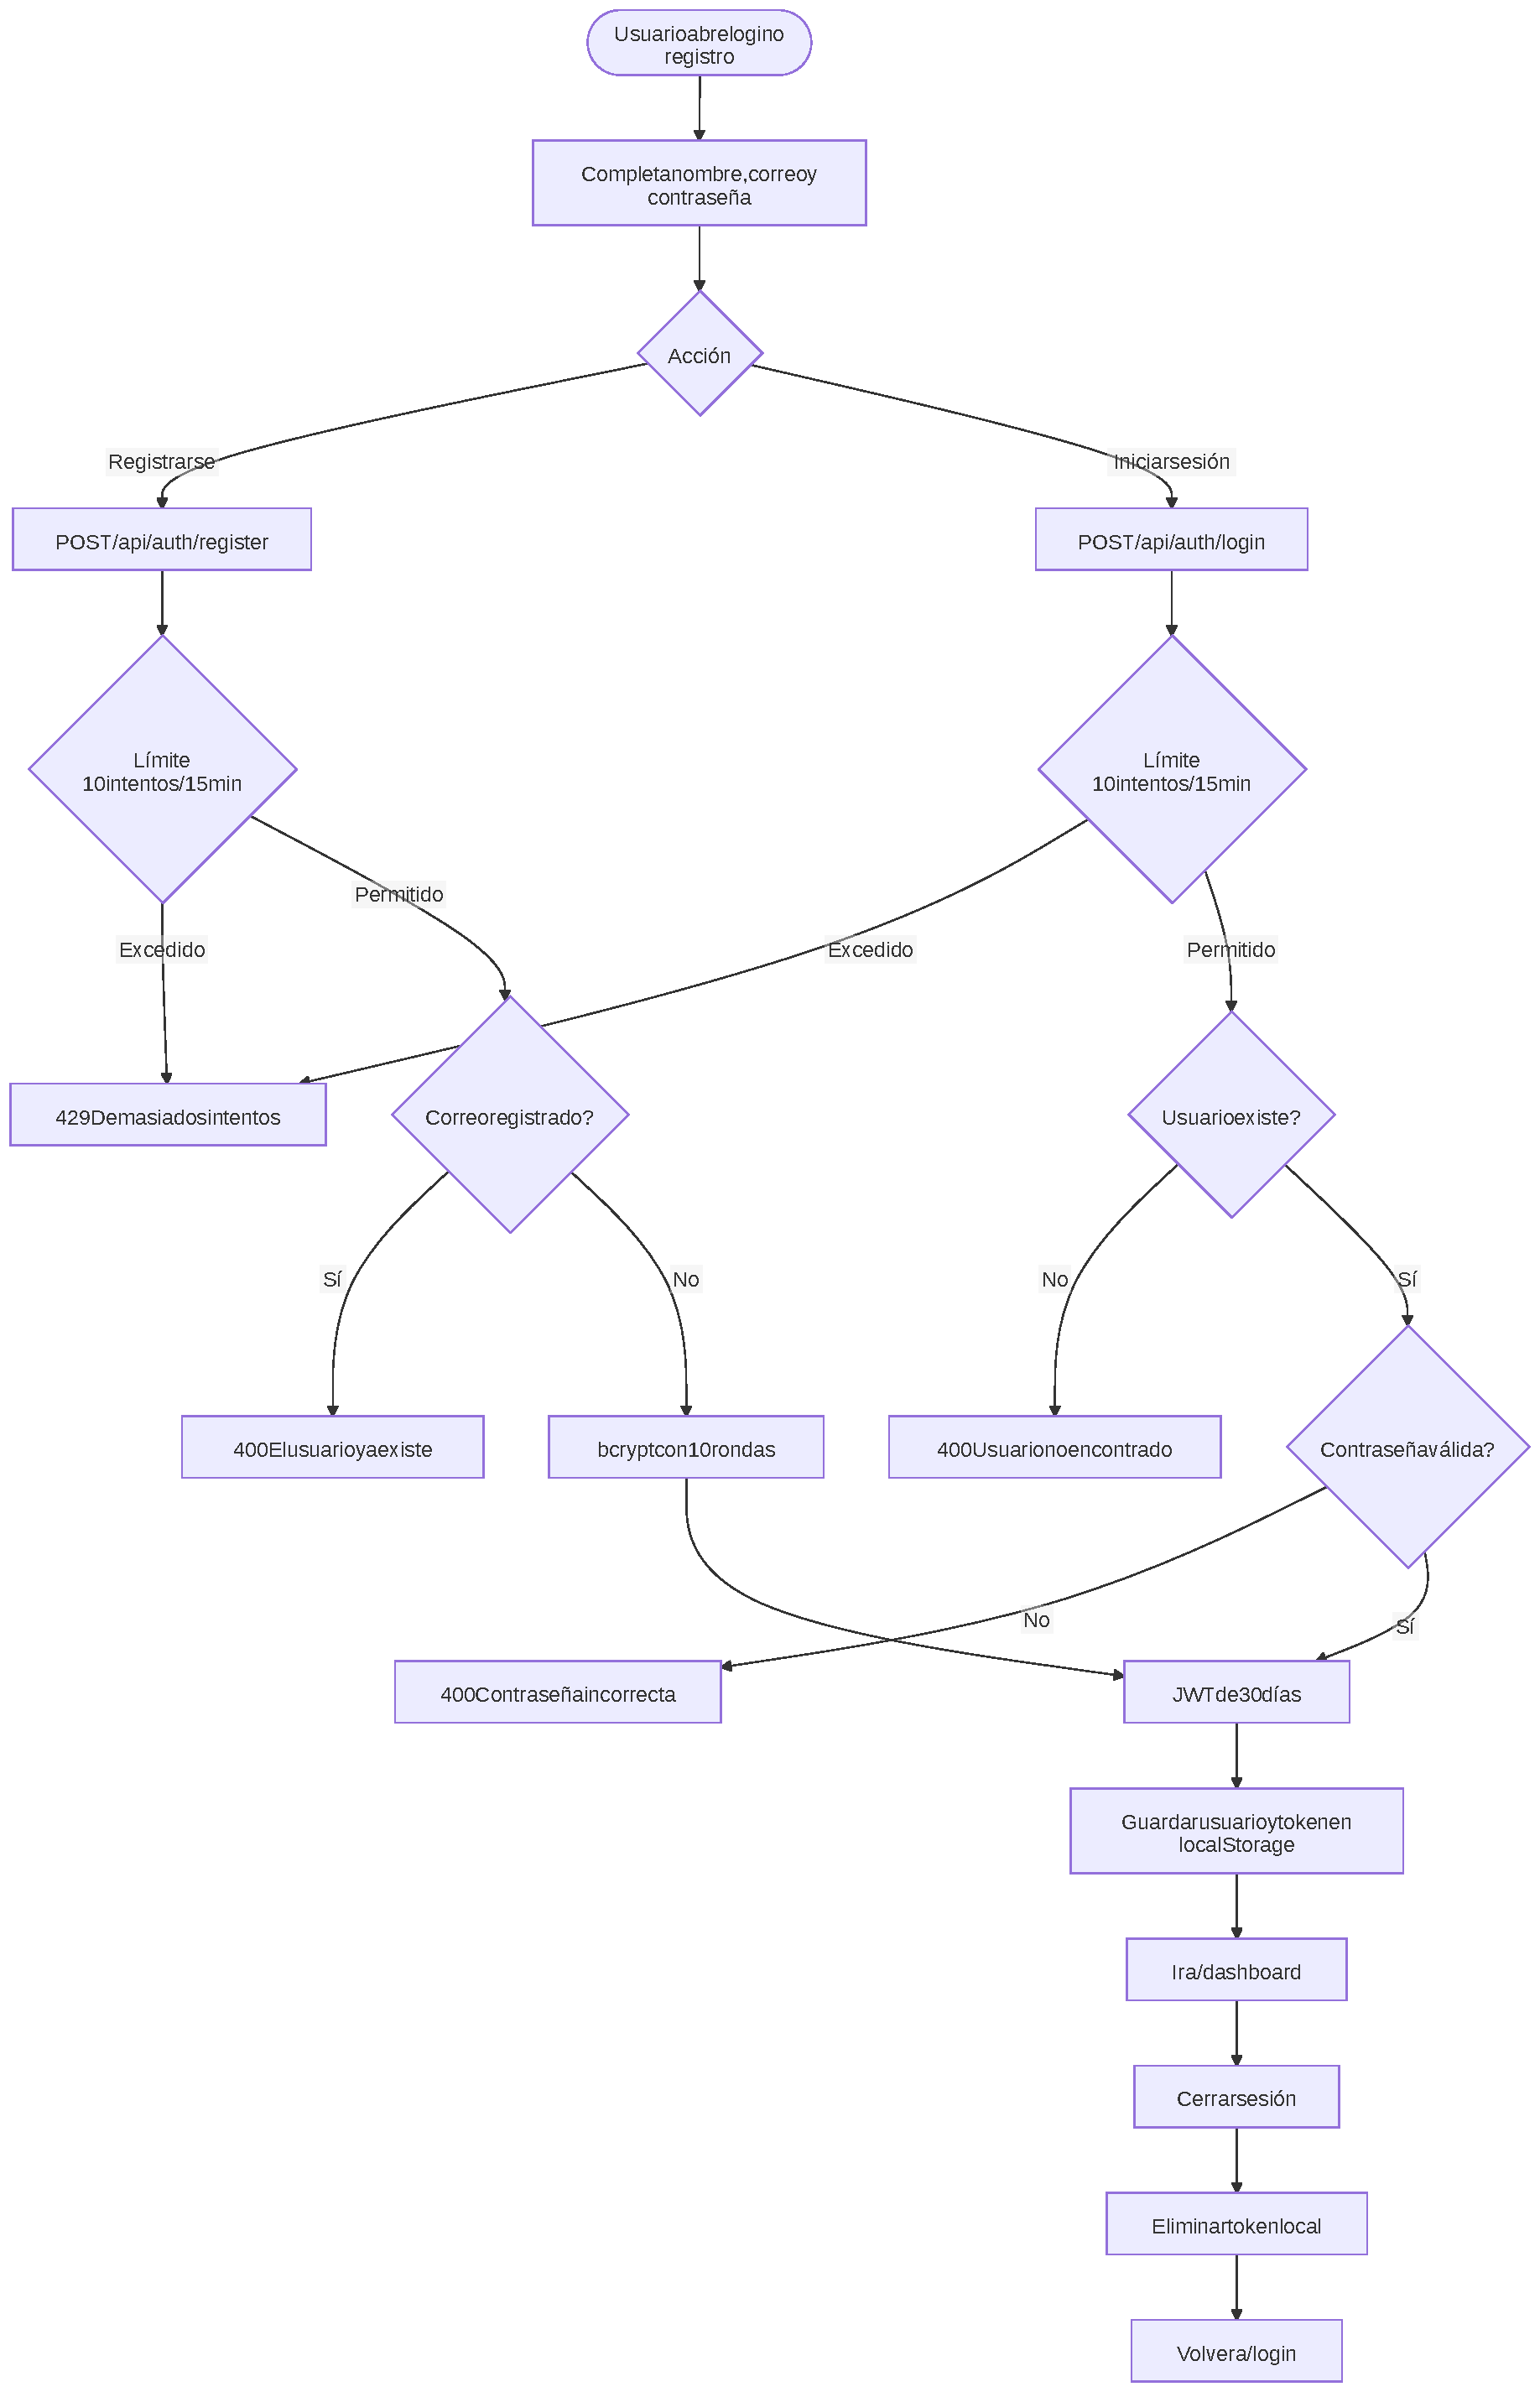
\includegraphics[width=0.72\textwidth, height=0.78\textheight, keepaspectratio]{figuras/flujo/flujo-autenticacion-y-sesion.pdf}
    \captionof{figure}{Diagrama de flujo del proceso de registro e inicio de sesión.}
    \label{fig:flujo-autenticacion}
\end{figure}

\subsection{Recetas y visibilidad}

\begin{figure}[H]
    \centering
    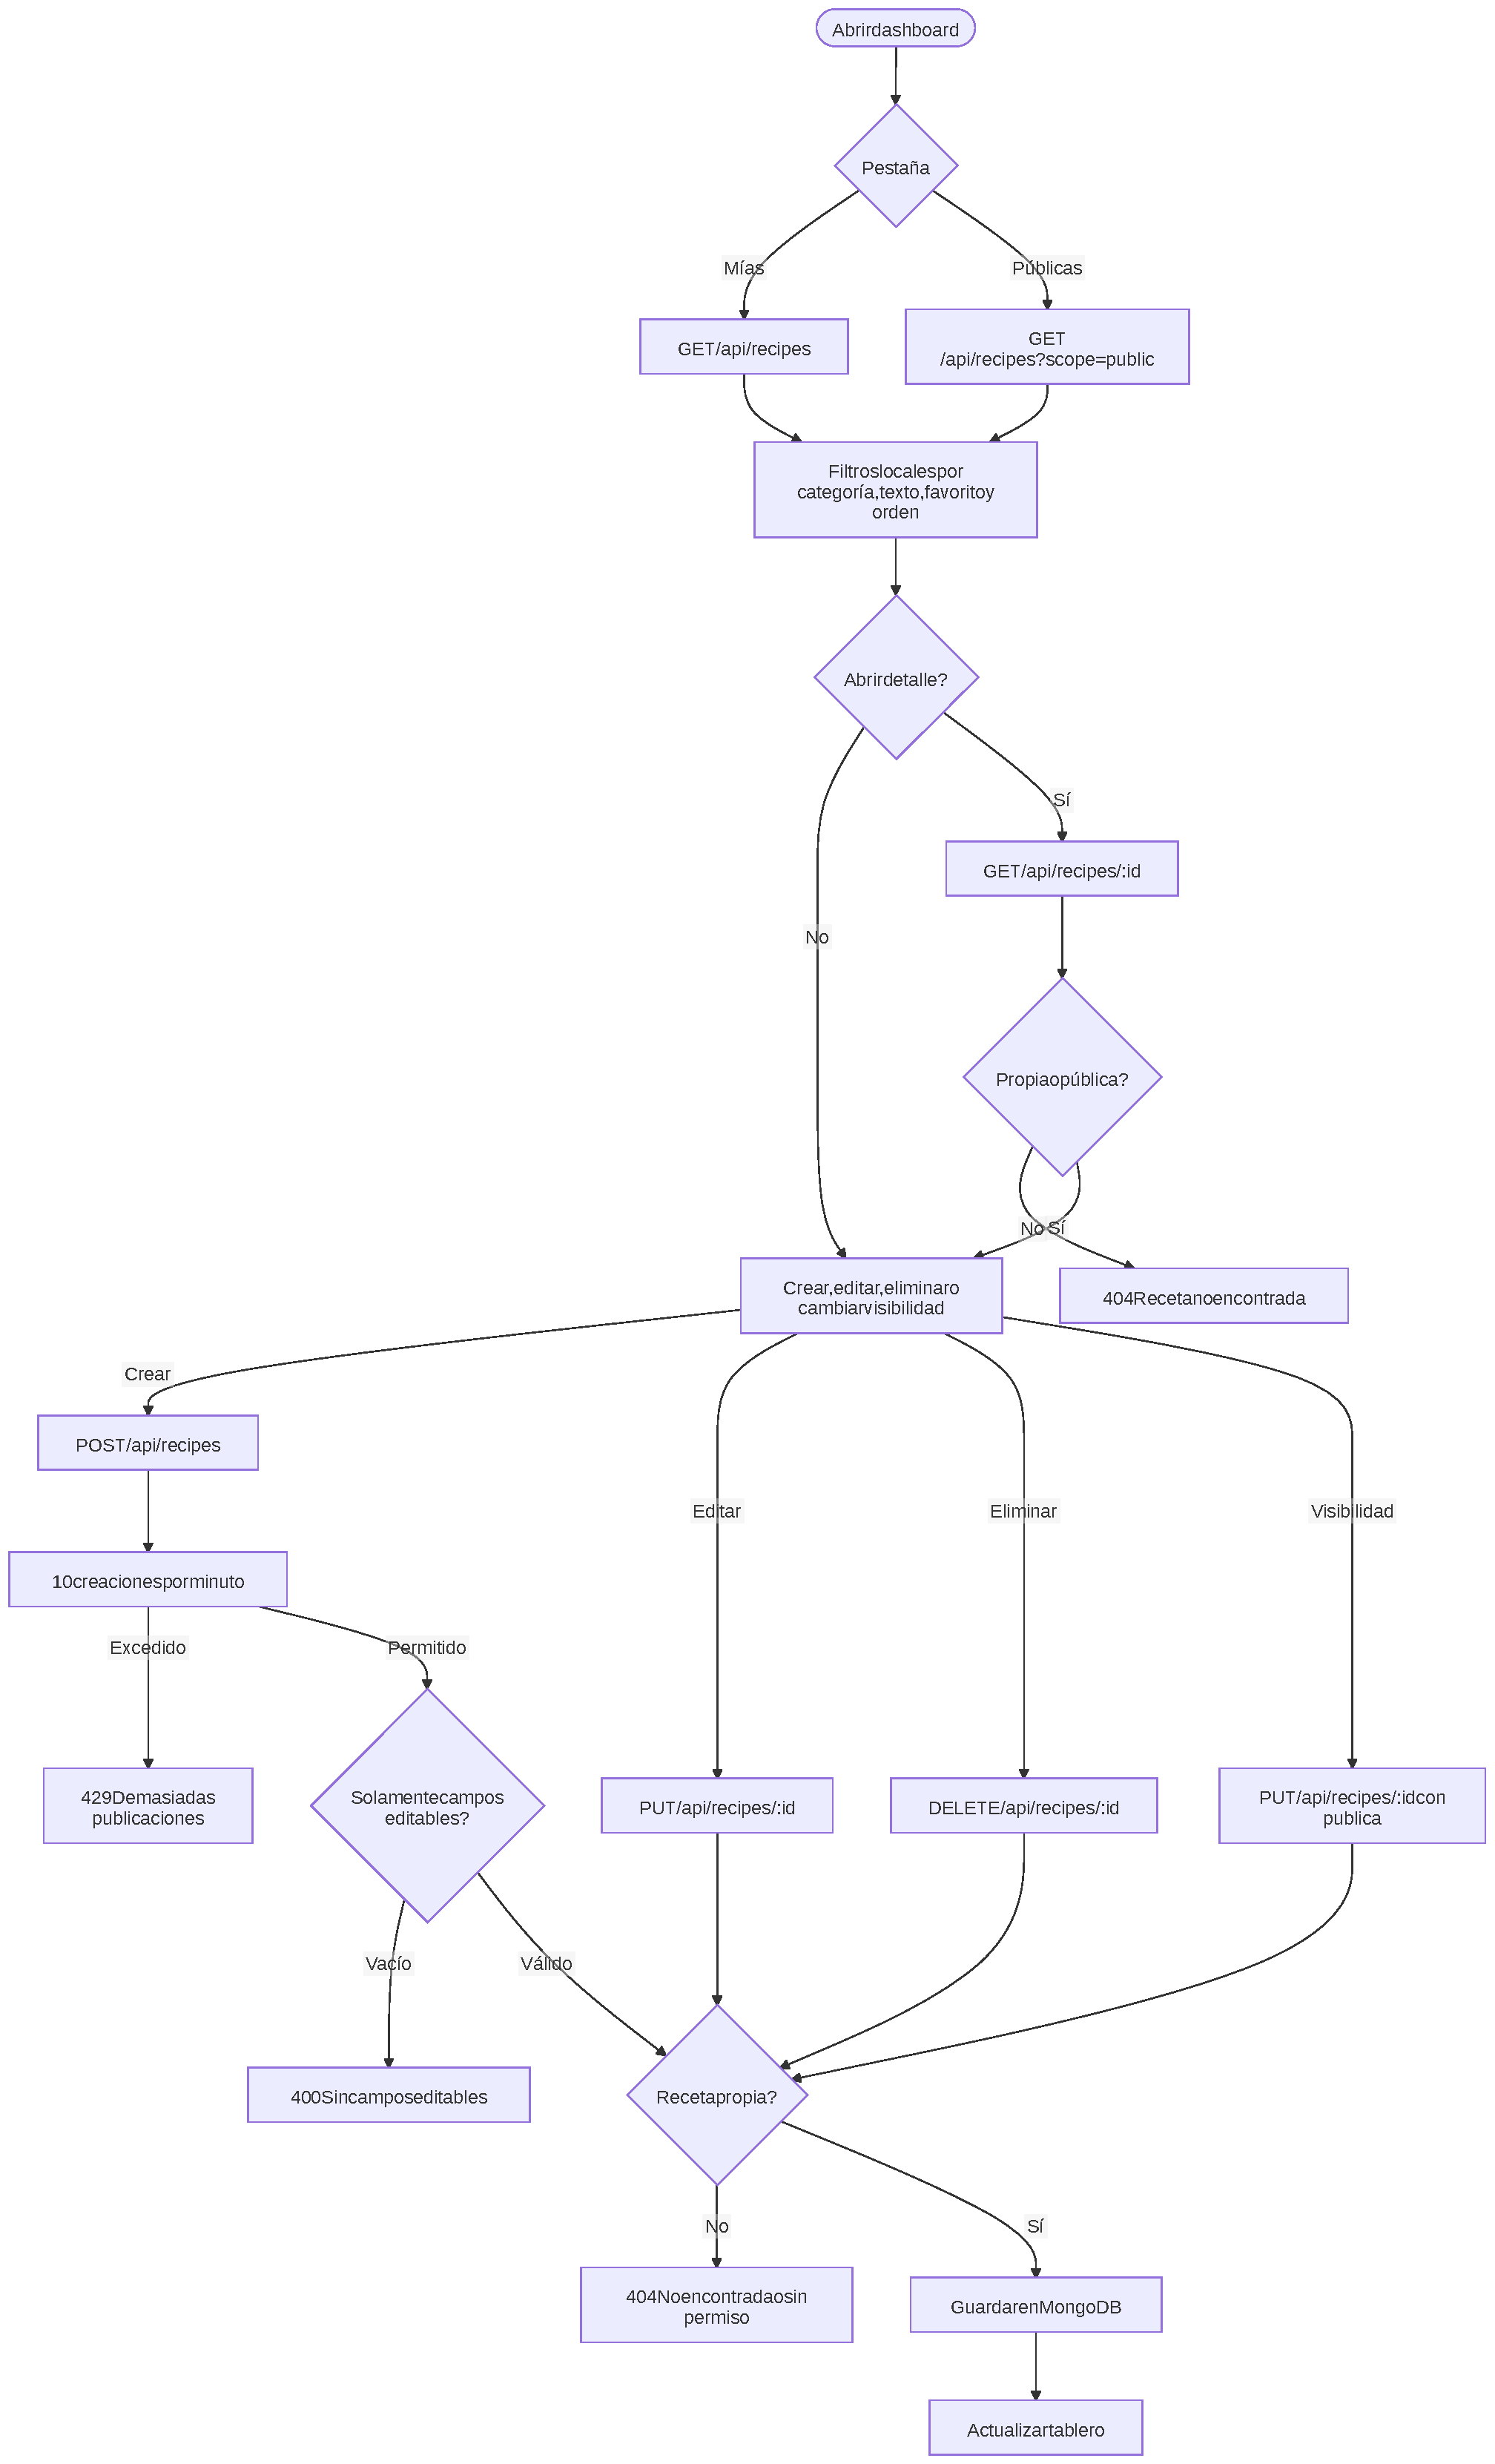
\includegraphics[width=0.72\textwidth, height=0.78\textheight, keepaspectratio]{figuras/flujo/flujo-recetas-y-visibilidad.pdf}
    \captionof{figure}{Diagrama de flujo del proceso de creación, consulta y visibilidad de recetas.}
    \label{fig:flujo-recetas}
\end{figure}

\subsection{Imágenes}

\begin{figure}[H]
    \centering
    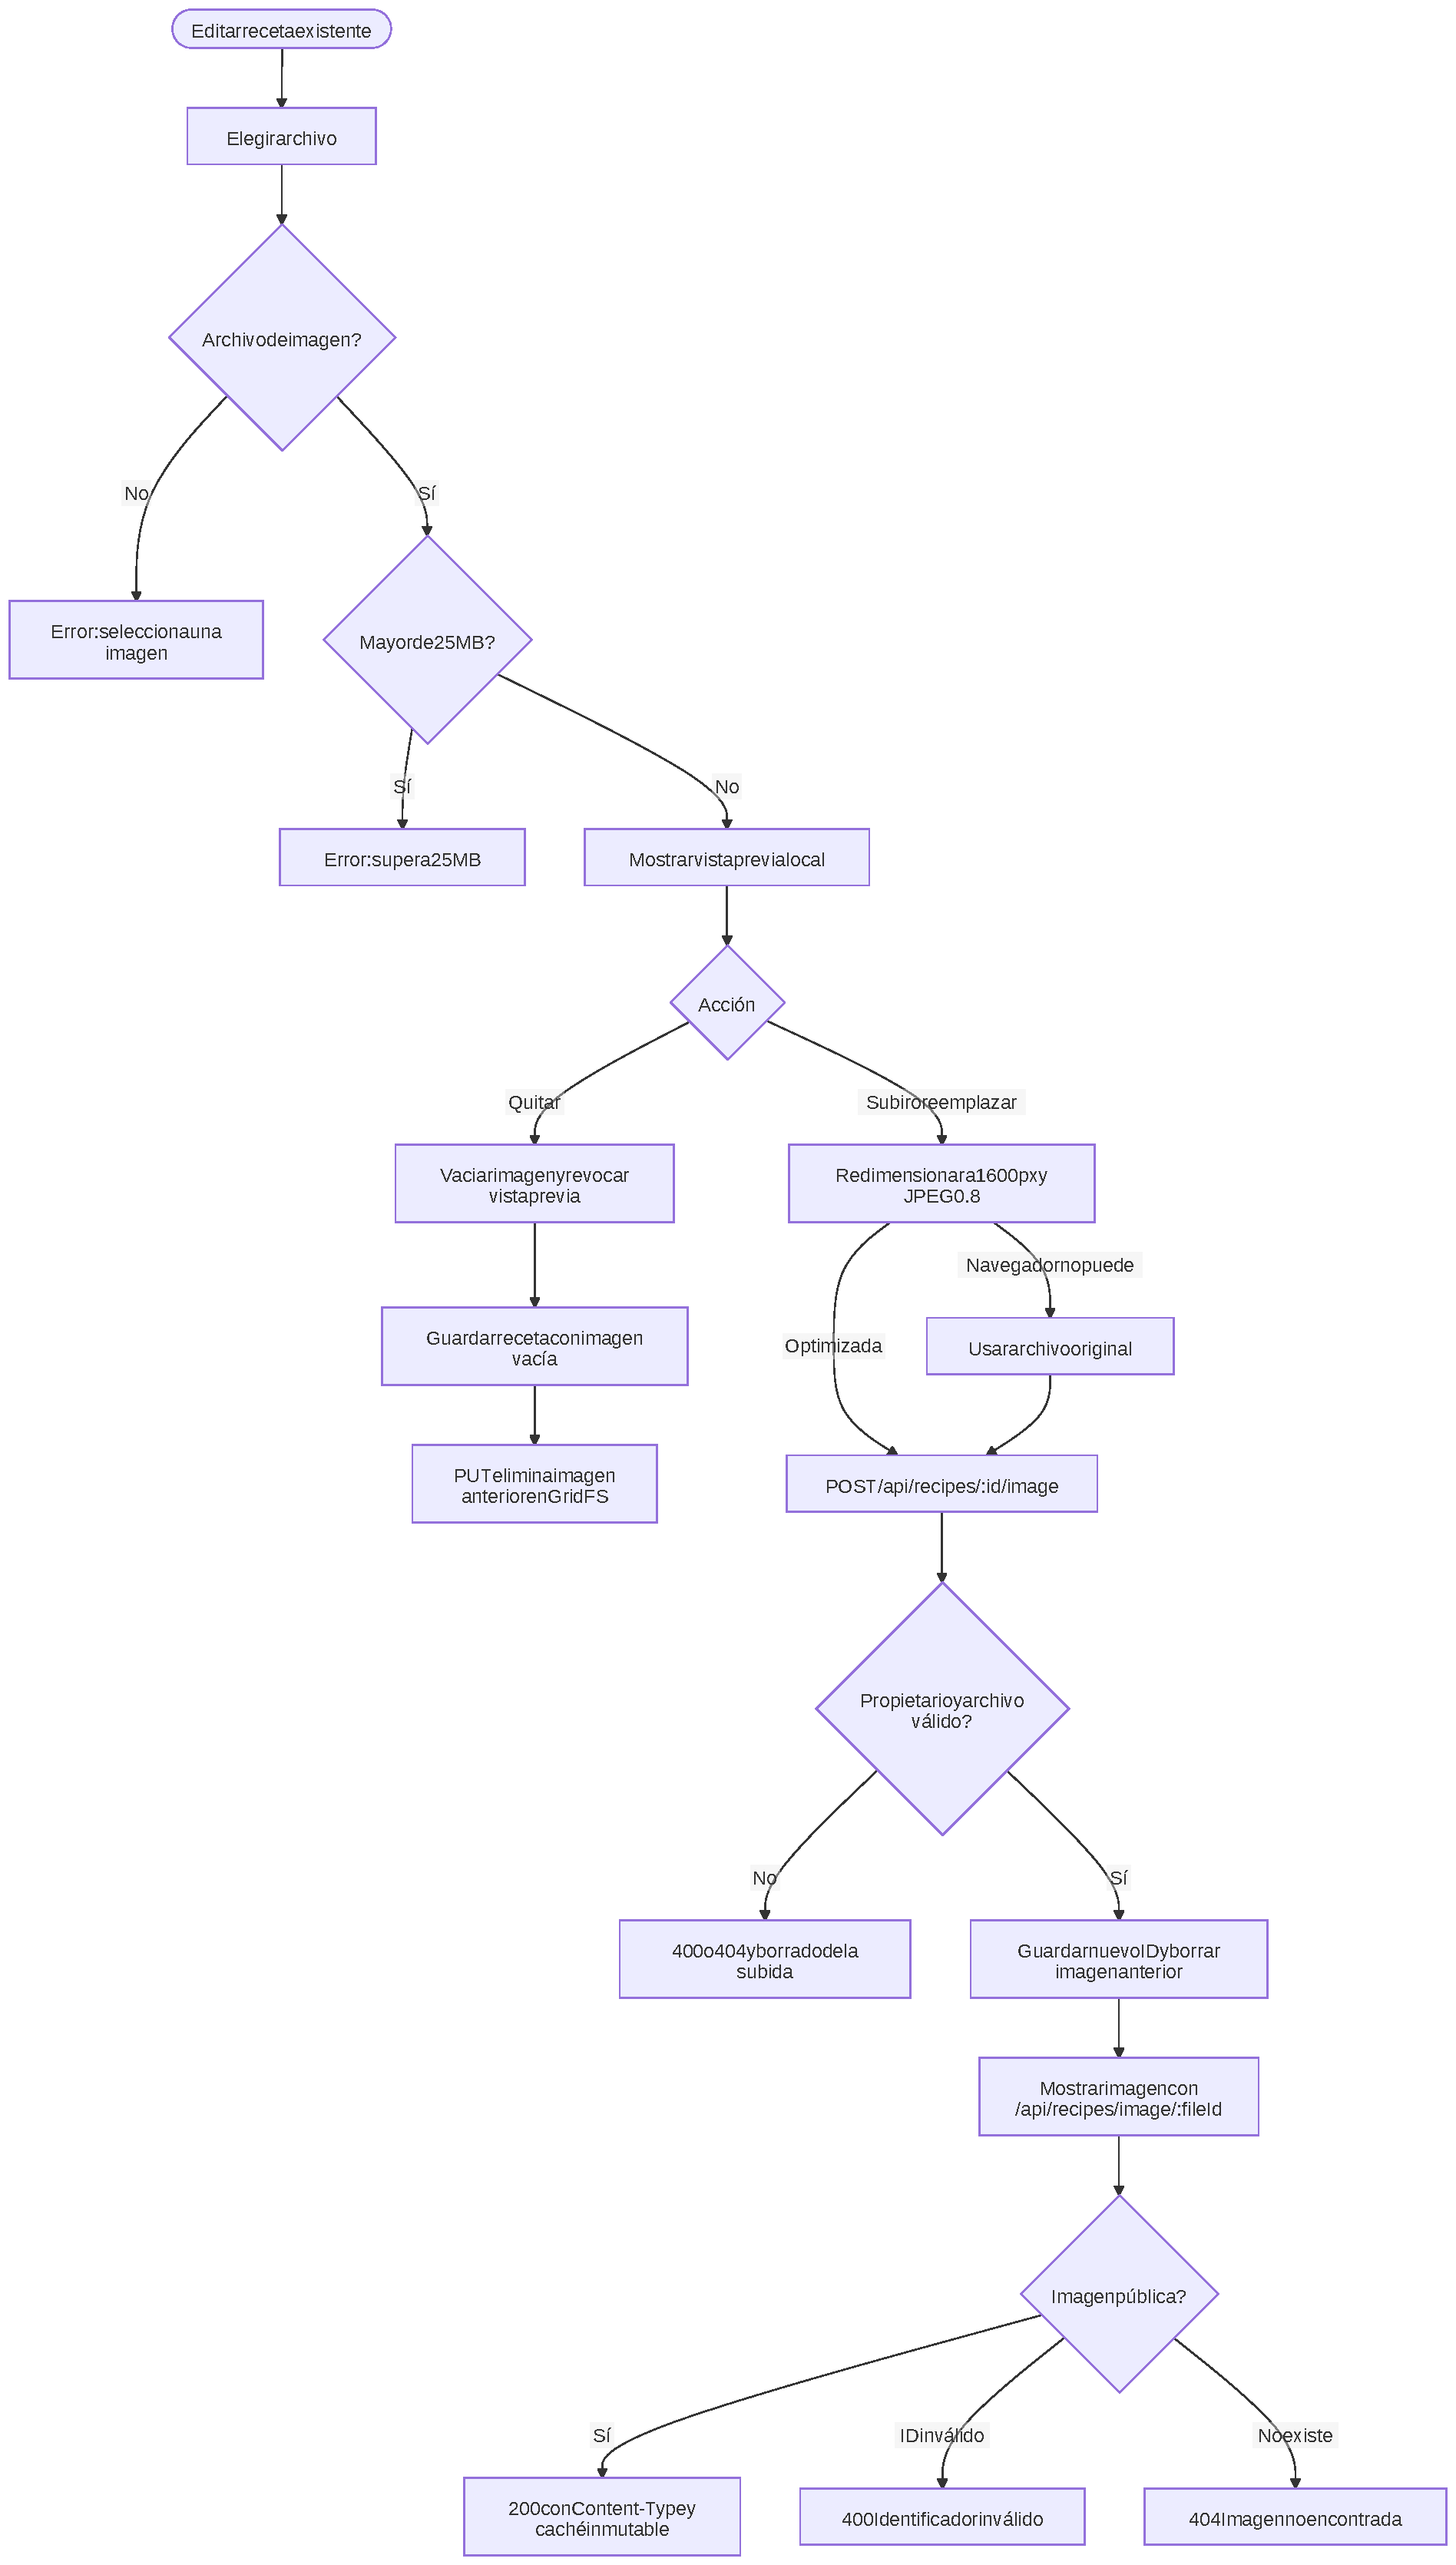
\includegraphics[width=0.72\textwidth, height=0.78\textheight, keepaspectratio]{figuras/flujo/flujo-imagenes.pdf}
    \captionof{figure}{Diagrama de flujo de la subida, reemplazo y eliminación de la imagen de una receta.}
    \label{fig:flujo-imagenes}
\end{figure}

\subsection{Interacciones sociales}

\begin{figure}[H]
    \centering
    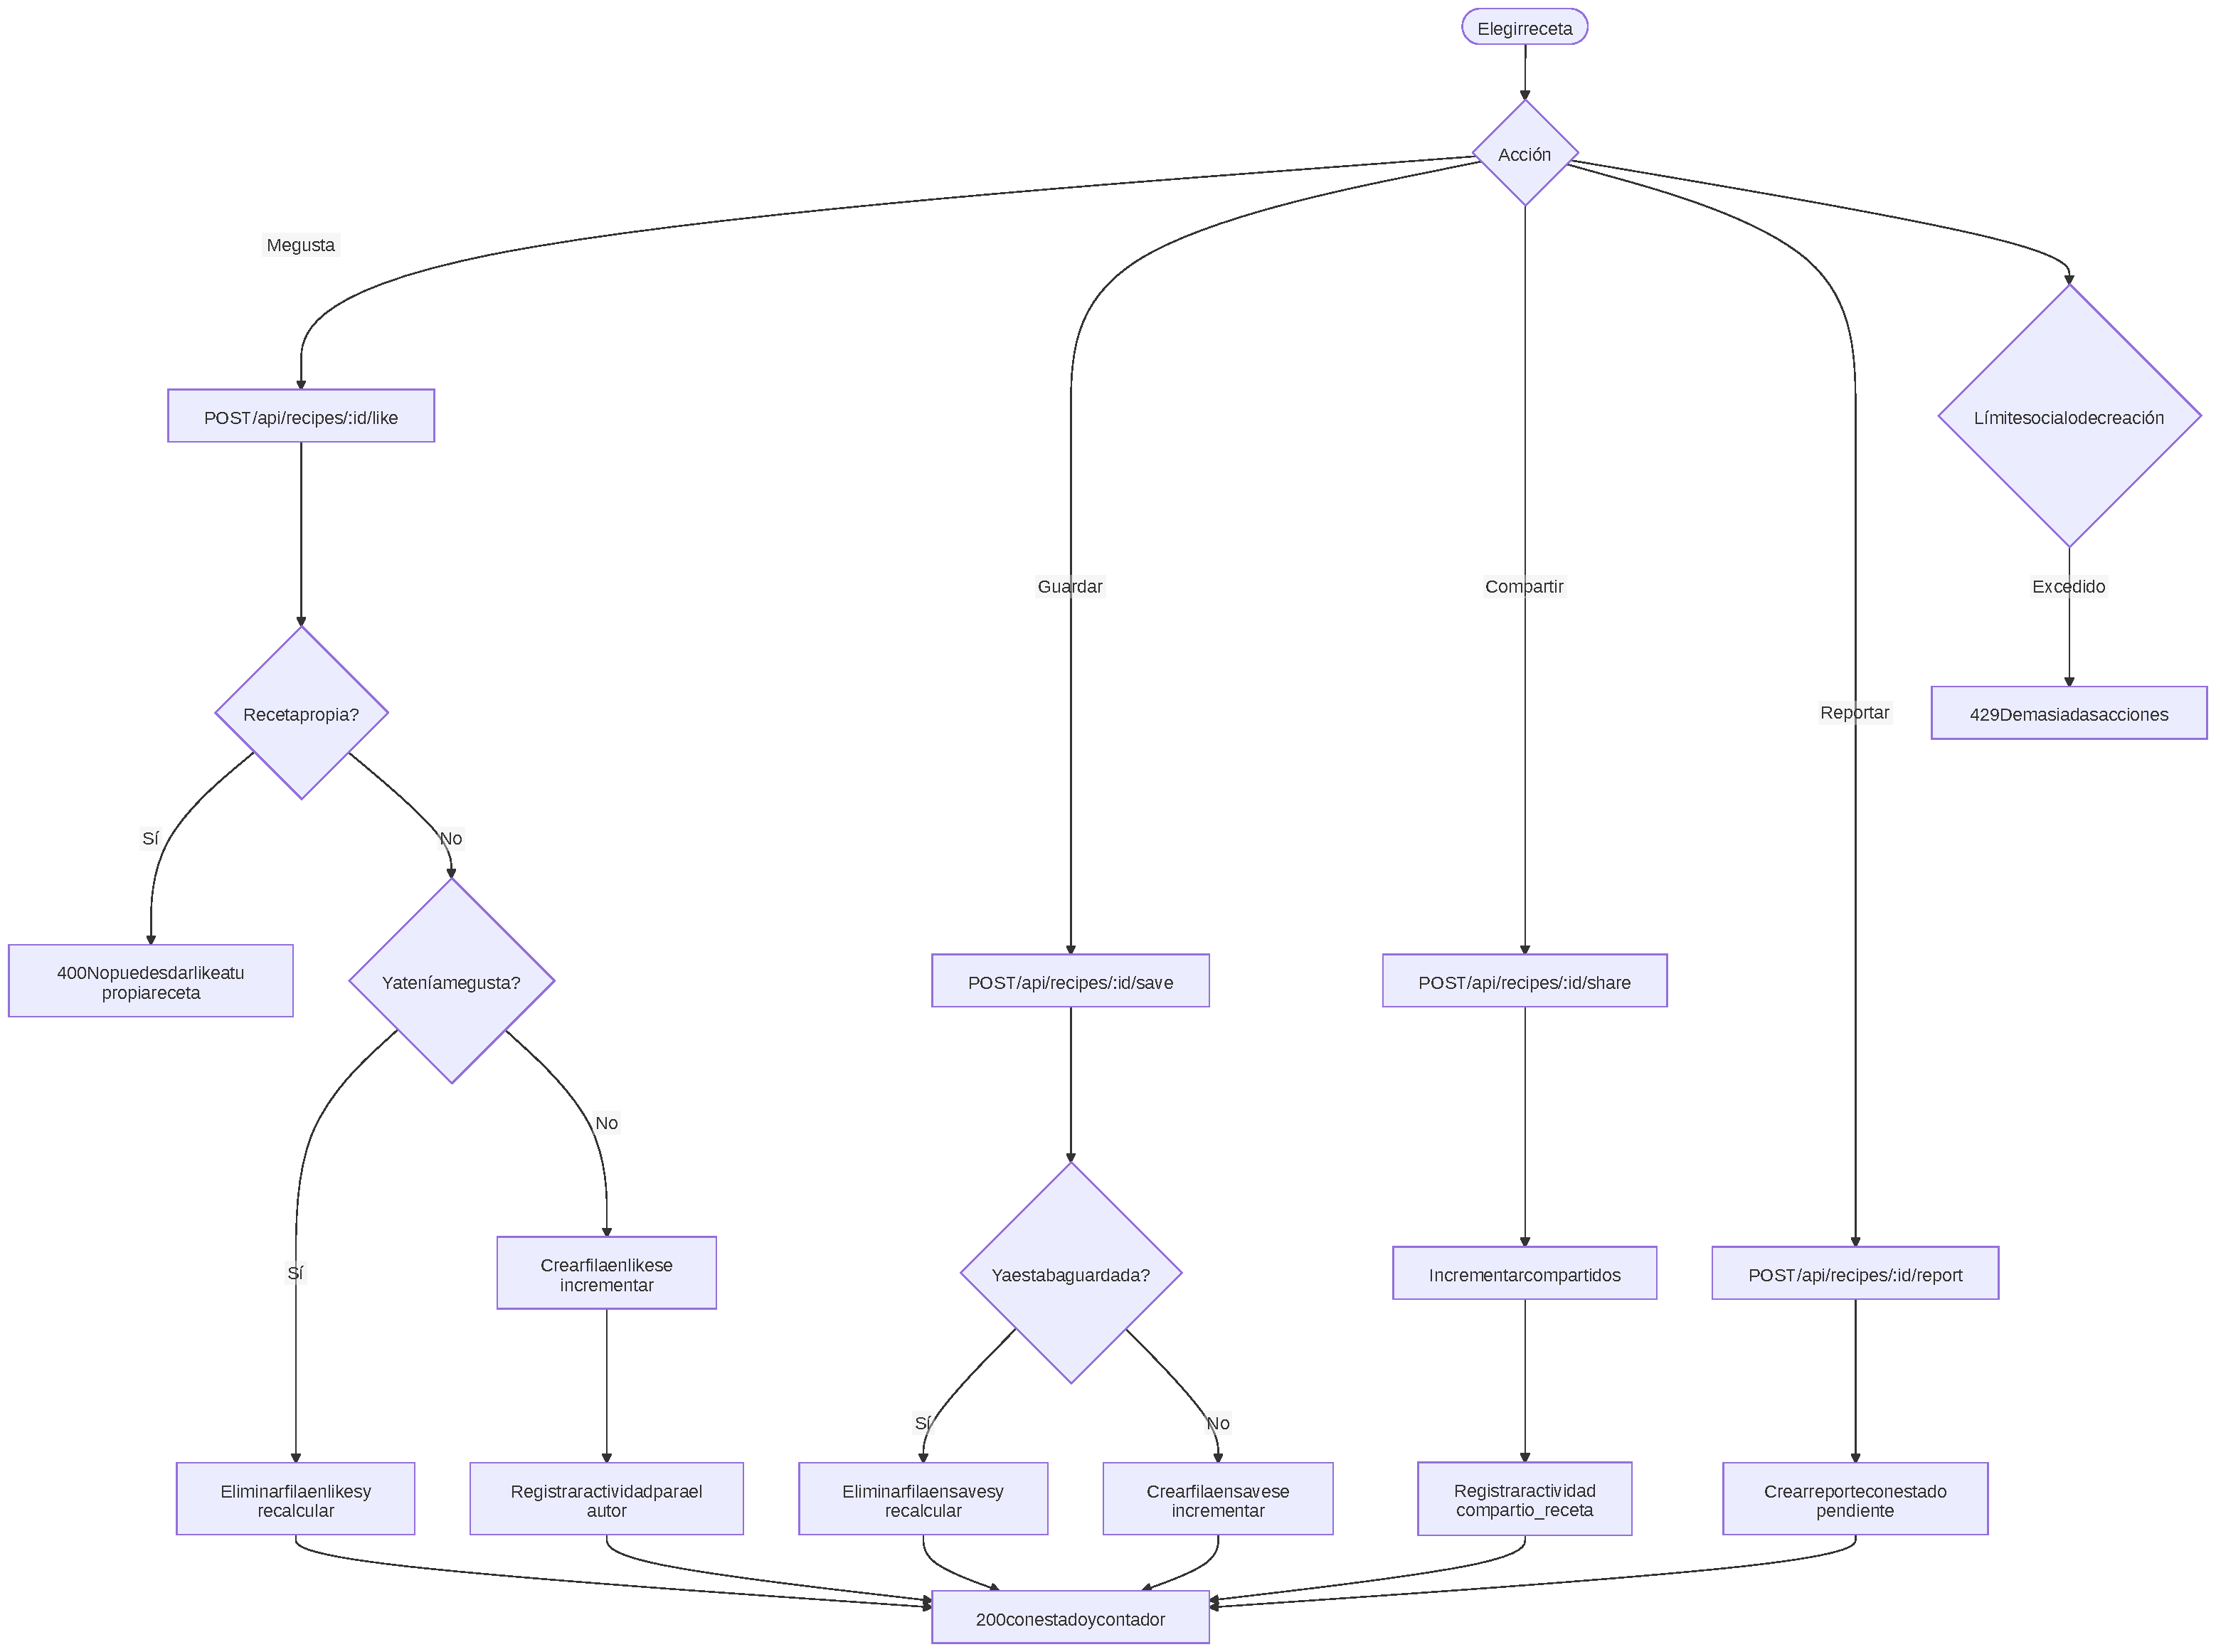
\includegraphics[width=0.72\textwidth, height=0.78\textheight, keepaspectratio]{figuras/flujo/flujo-interacciones-sociales.pdf}
    \captionof{figure}{Diagrama de flujo de las interacciones sociales sobre una receta.}
    \label{fig:flujo-interacciones}
\end{figure}

\subsection{Comentarios y reseñas}

\begin{figure}[H]
    \centering
    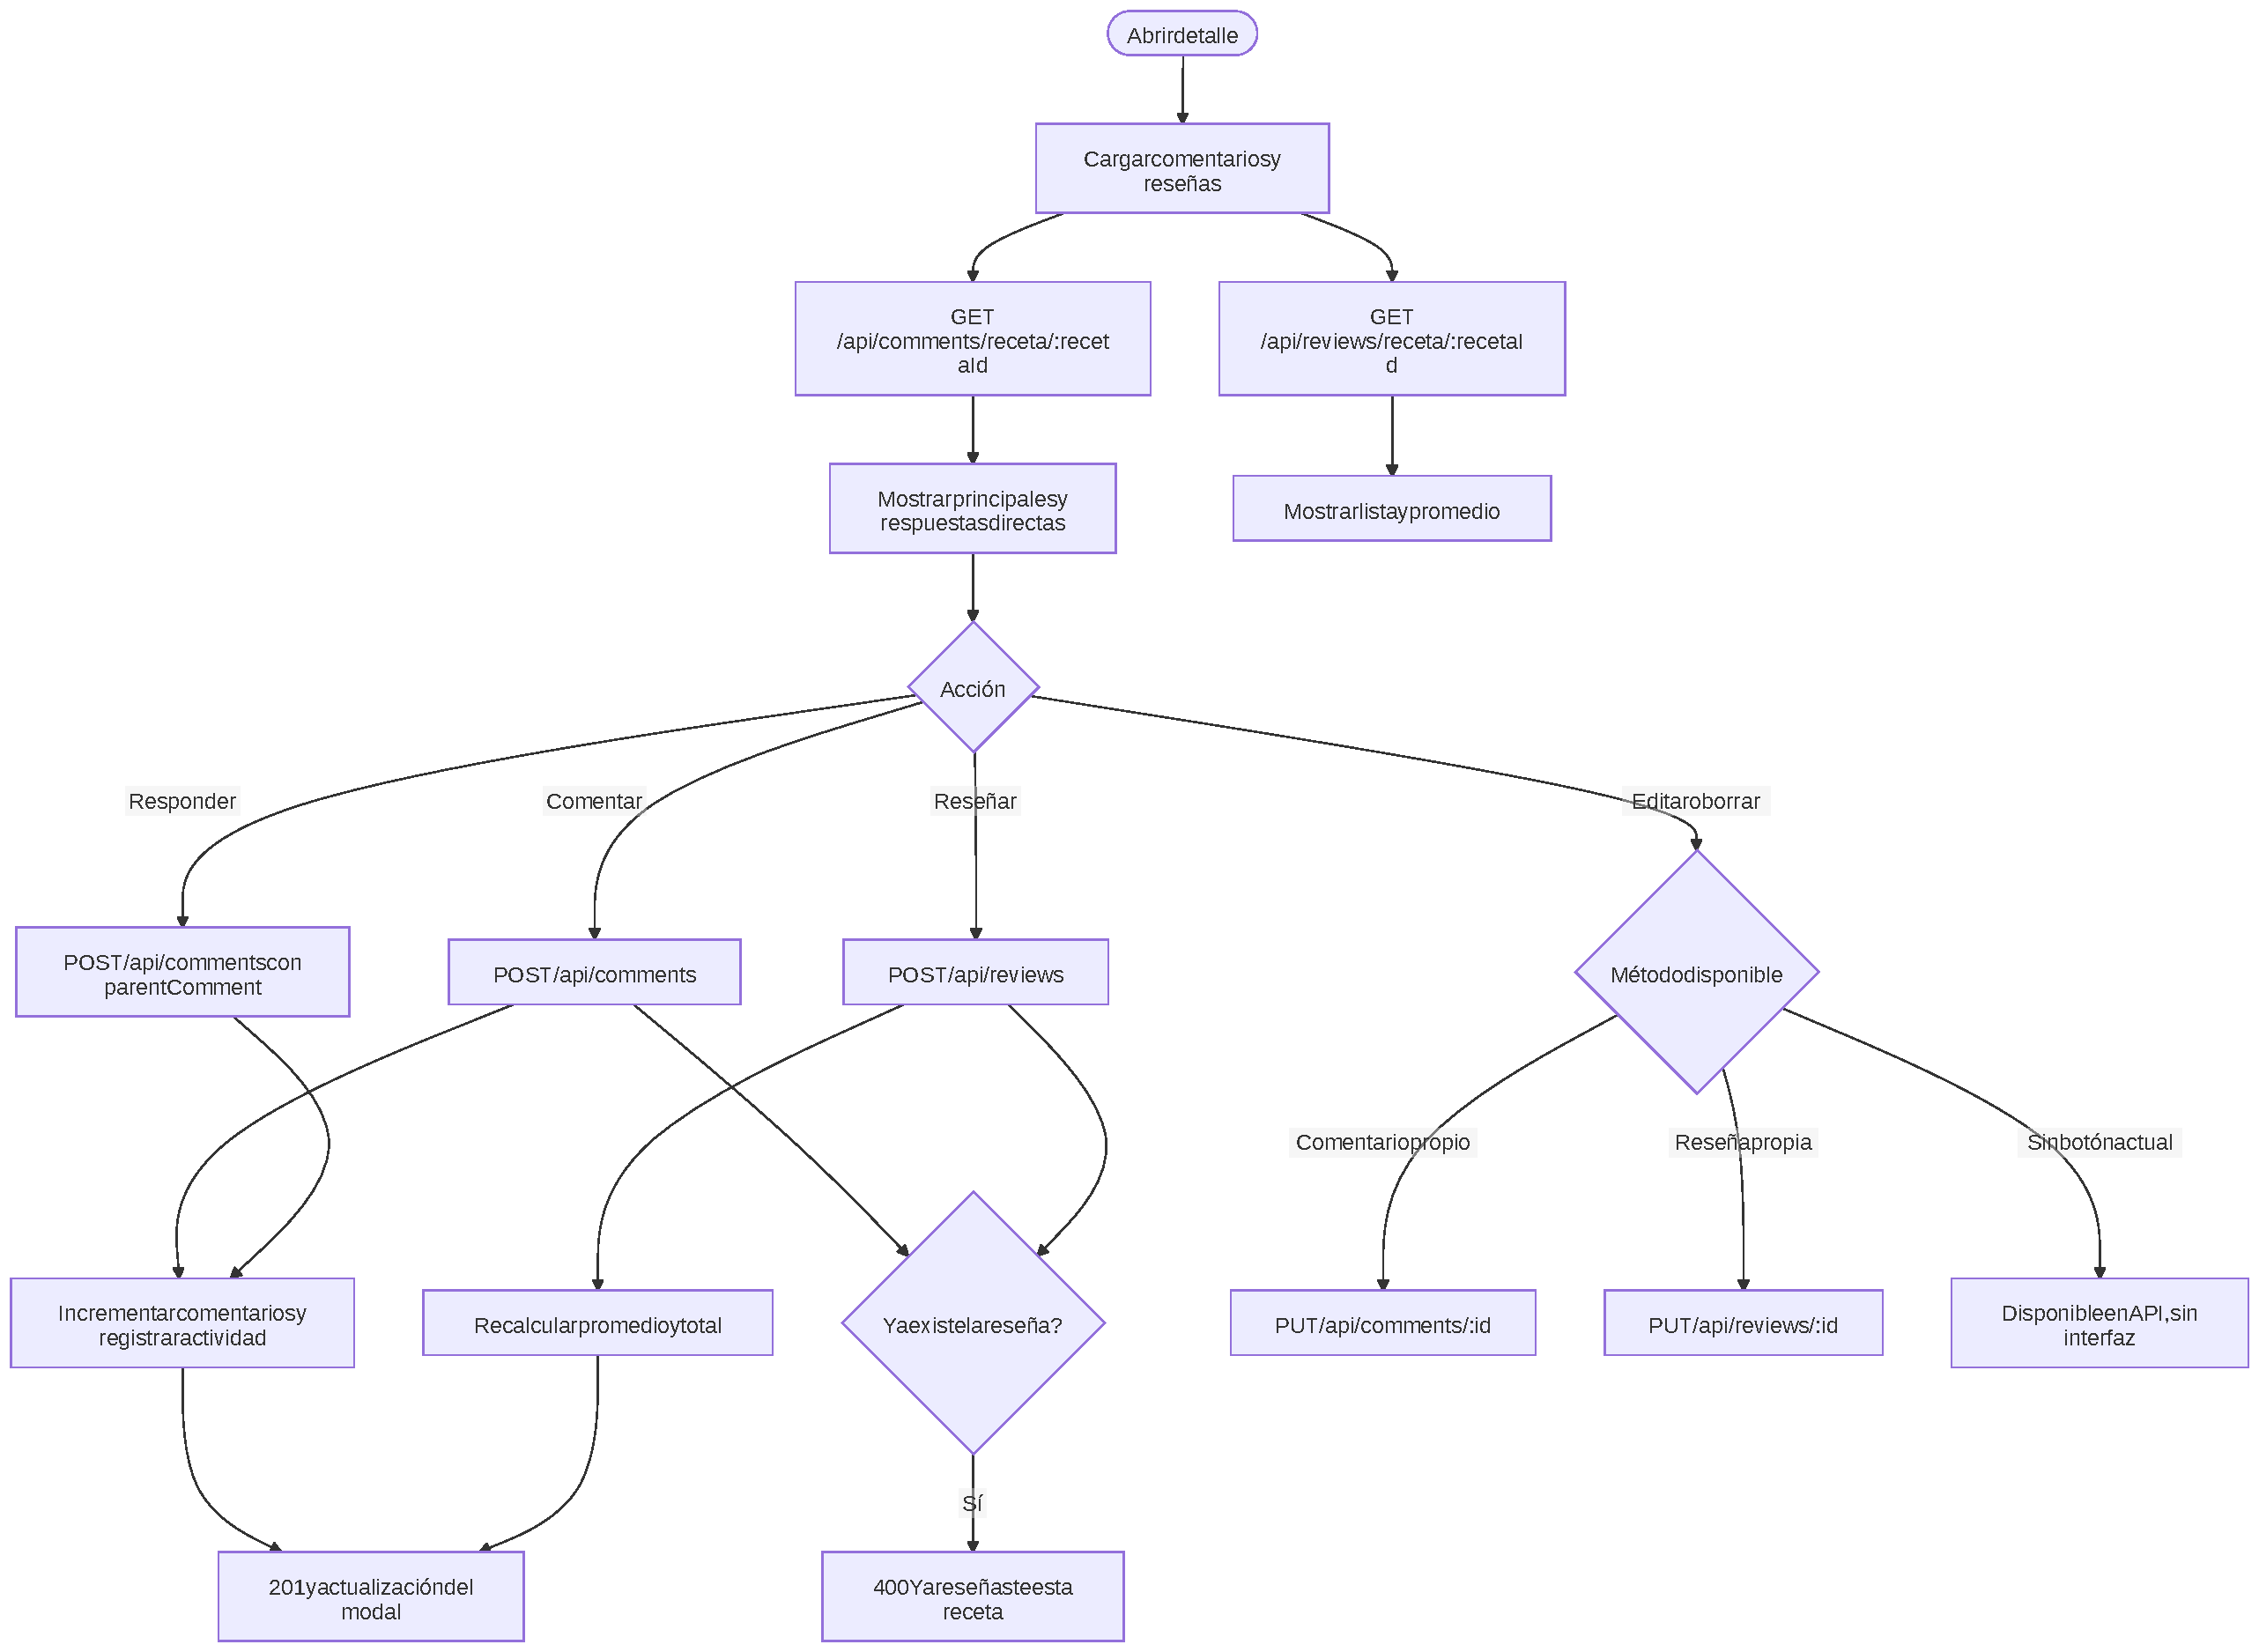
\includegraphics[width=0.72\textwidth, height=0.78\textheight, keepaspectratio]{figuras/flujo/flujo-comentarios-y-resenas.pdf}
    \captionof{figure}{Diagrama de flujo del proceso de comentarios y reseñas.}
    \label{fig:flujo-comentarios}
\end{figure}

\subsection{Seguimiento, feed y notificaciones}

\begin{figure}[H]
    \centering
    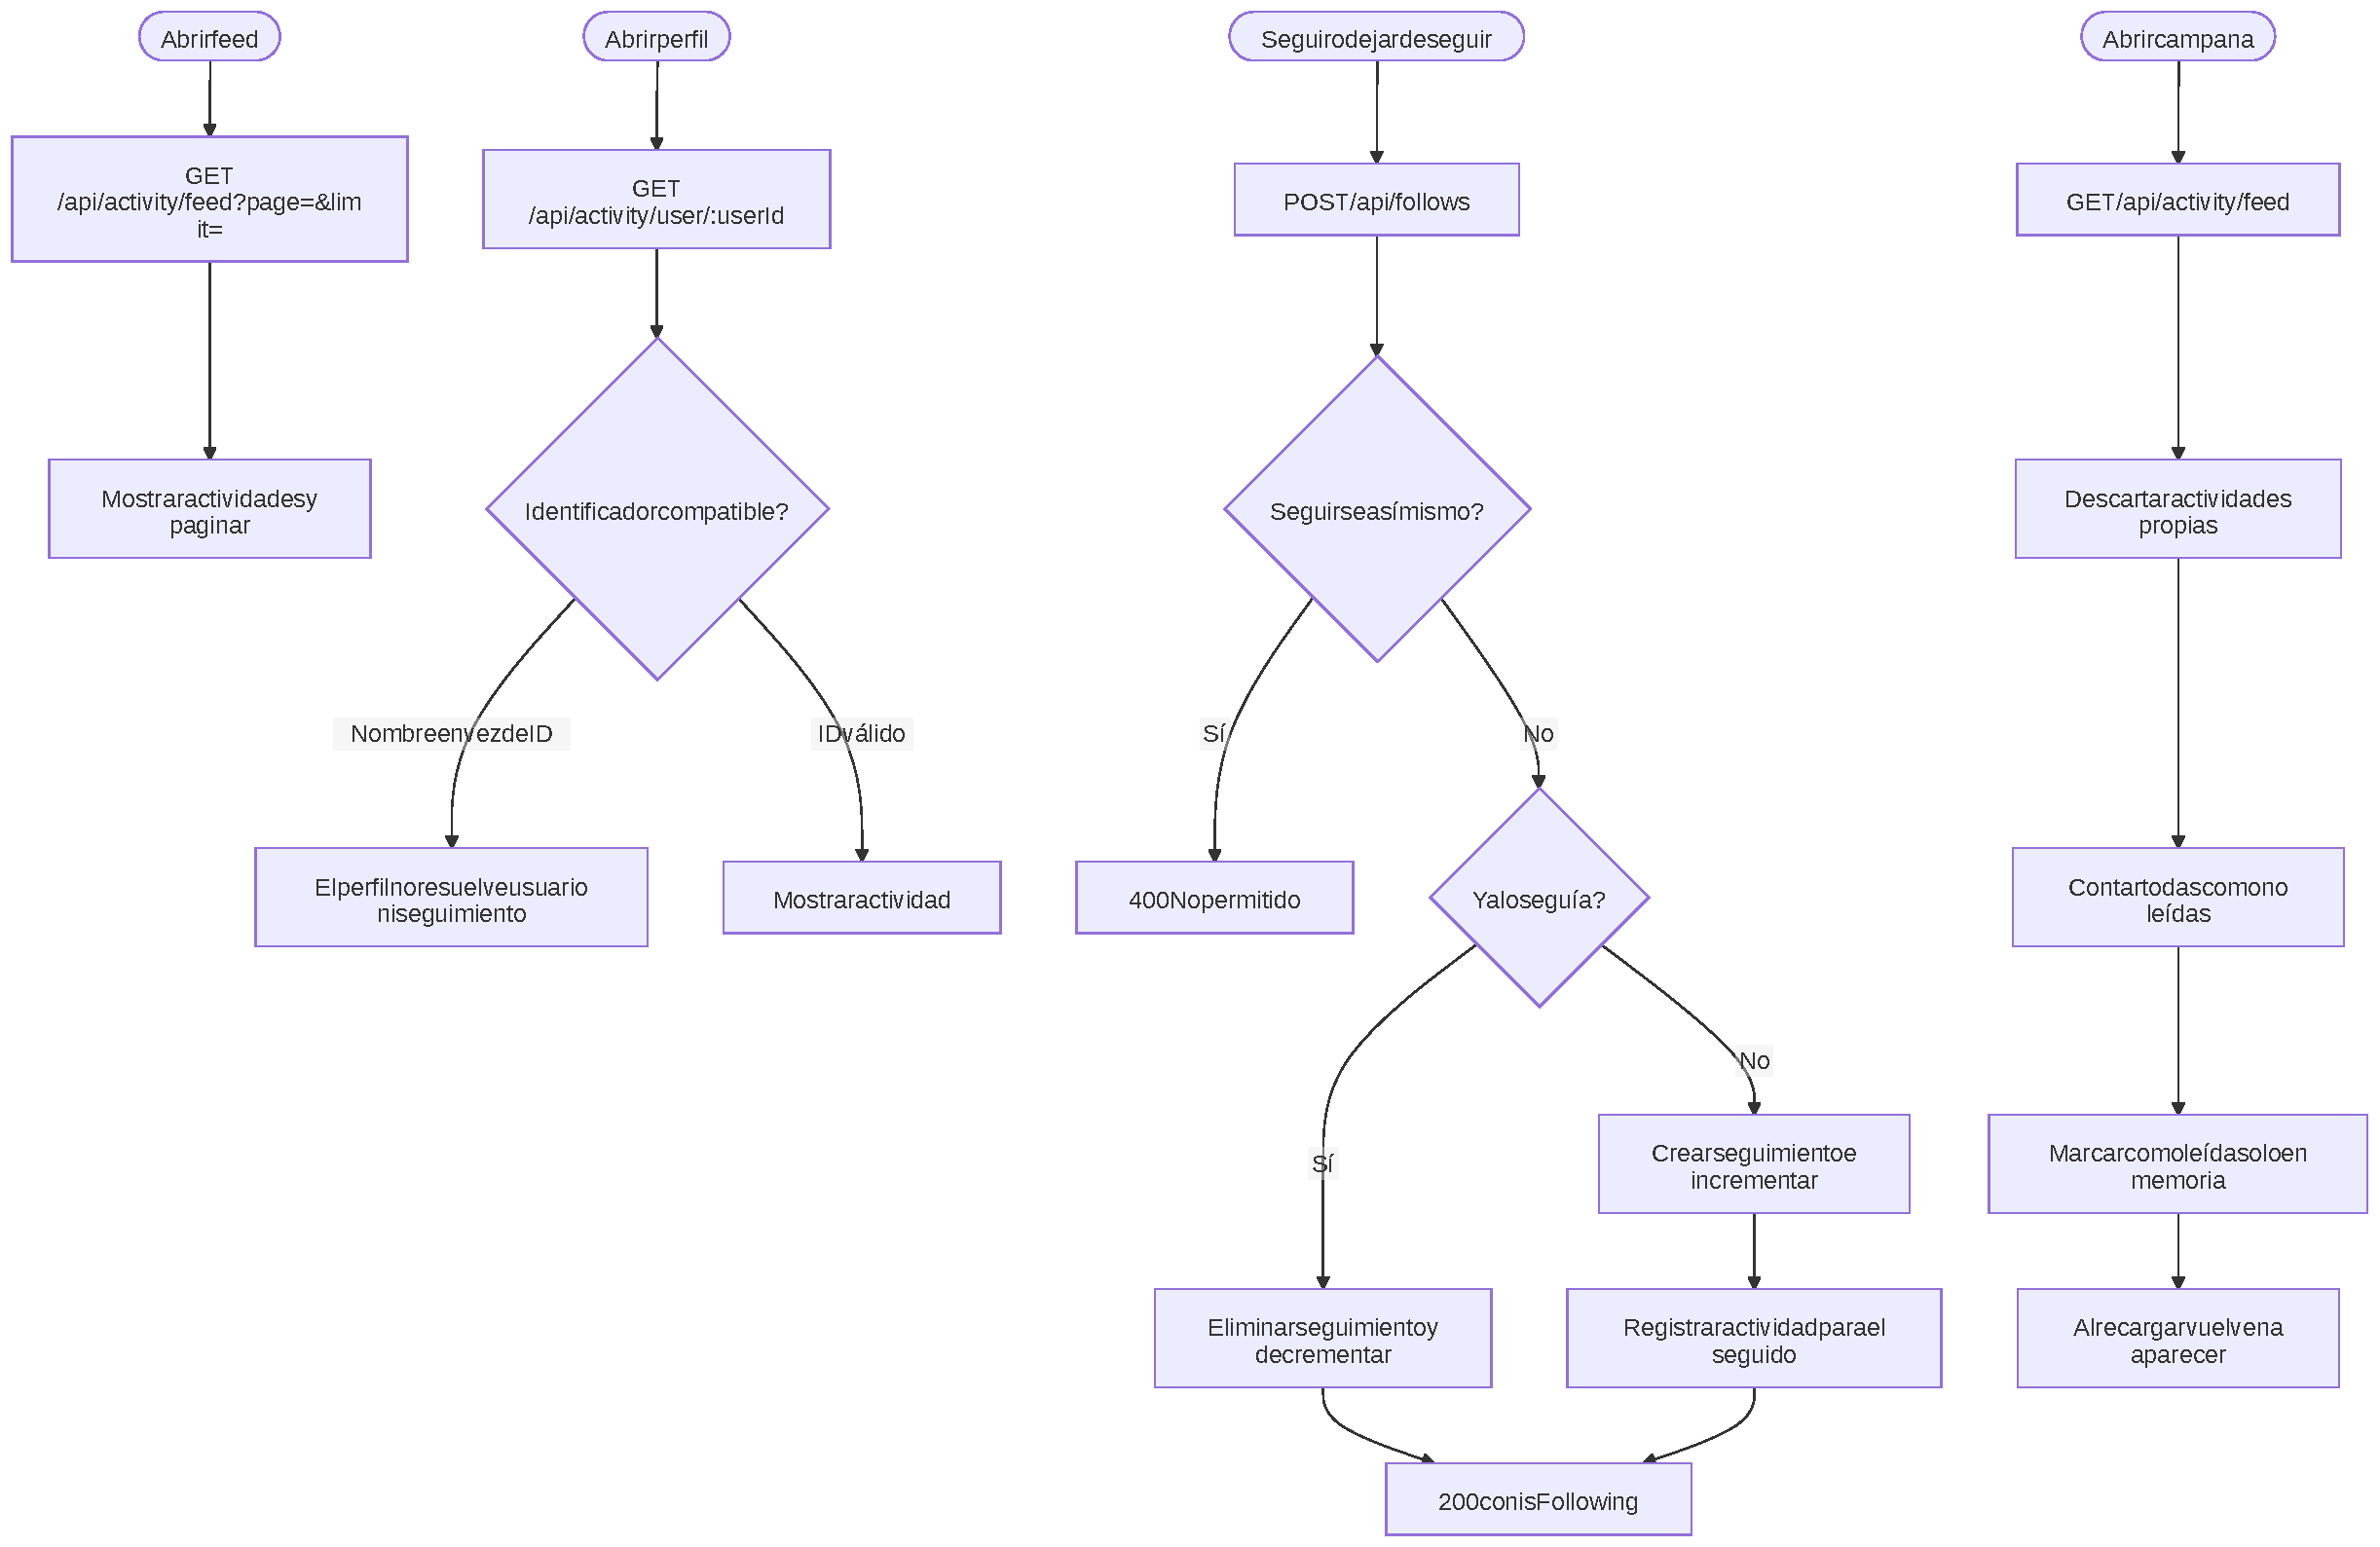
\includegraphics[width=0.72\textwidth, height=0.78\textheight, keepaspectratio]{figuras/flujo/flujo-seguimiento-feed-y-notificaciones.pdf}
    \captionof{figure}{Diagrama de flujo del seguimiento, el feed y la campana de notificaciones.}
    \label{fig:flujo-seguimiento}
\end{figure}

\subsection{Visión general del sistema}

\begin{figure}[H]
    \centering
    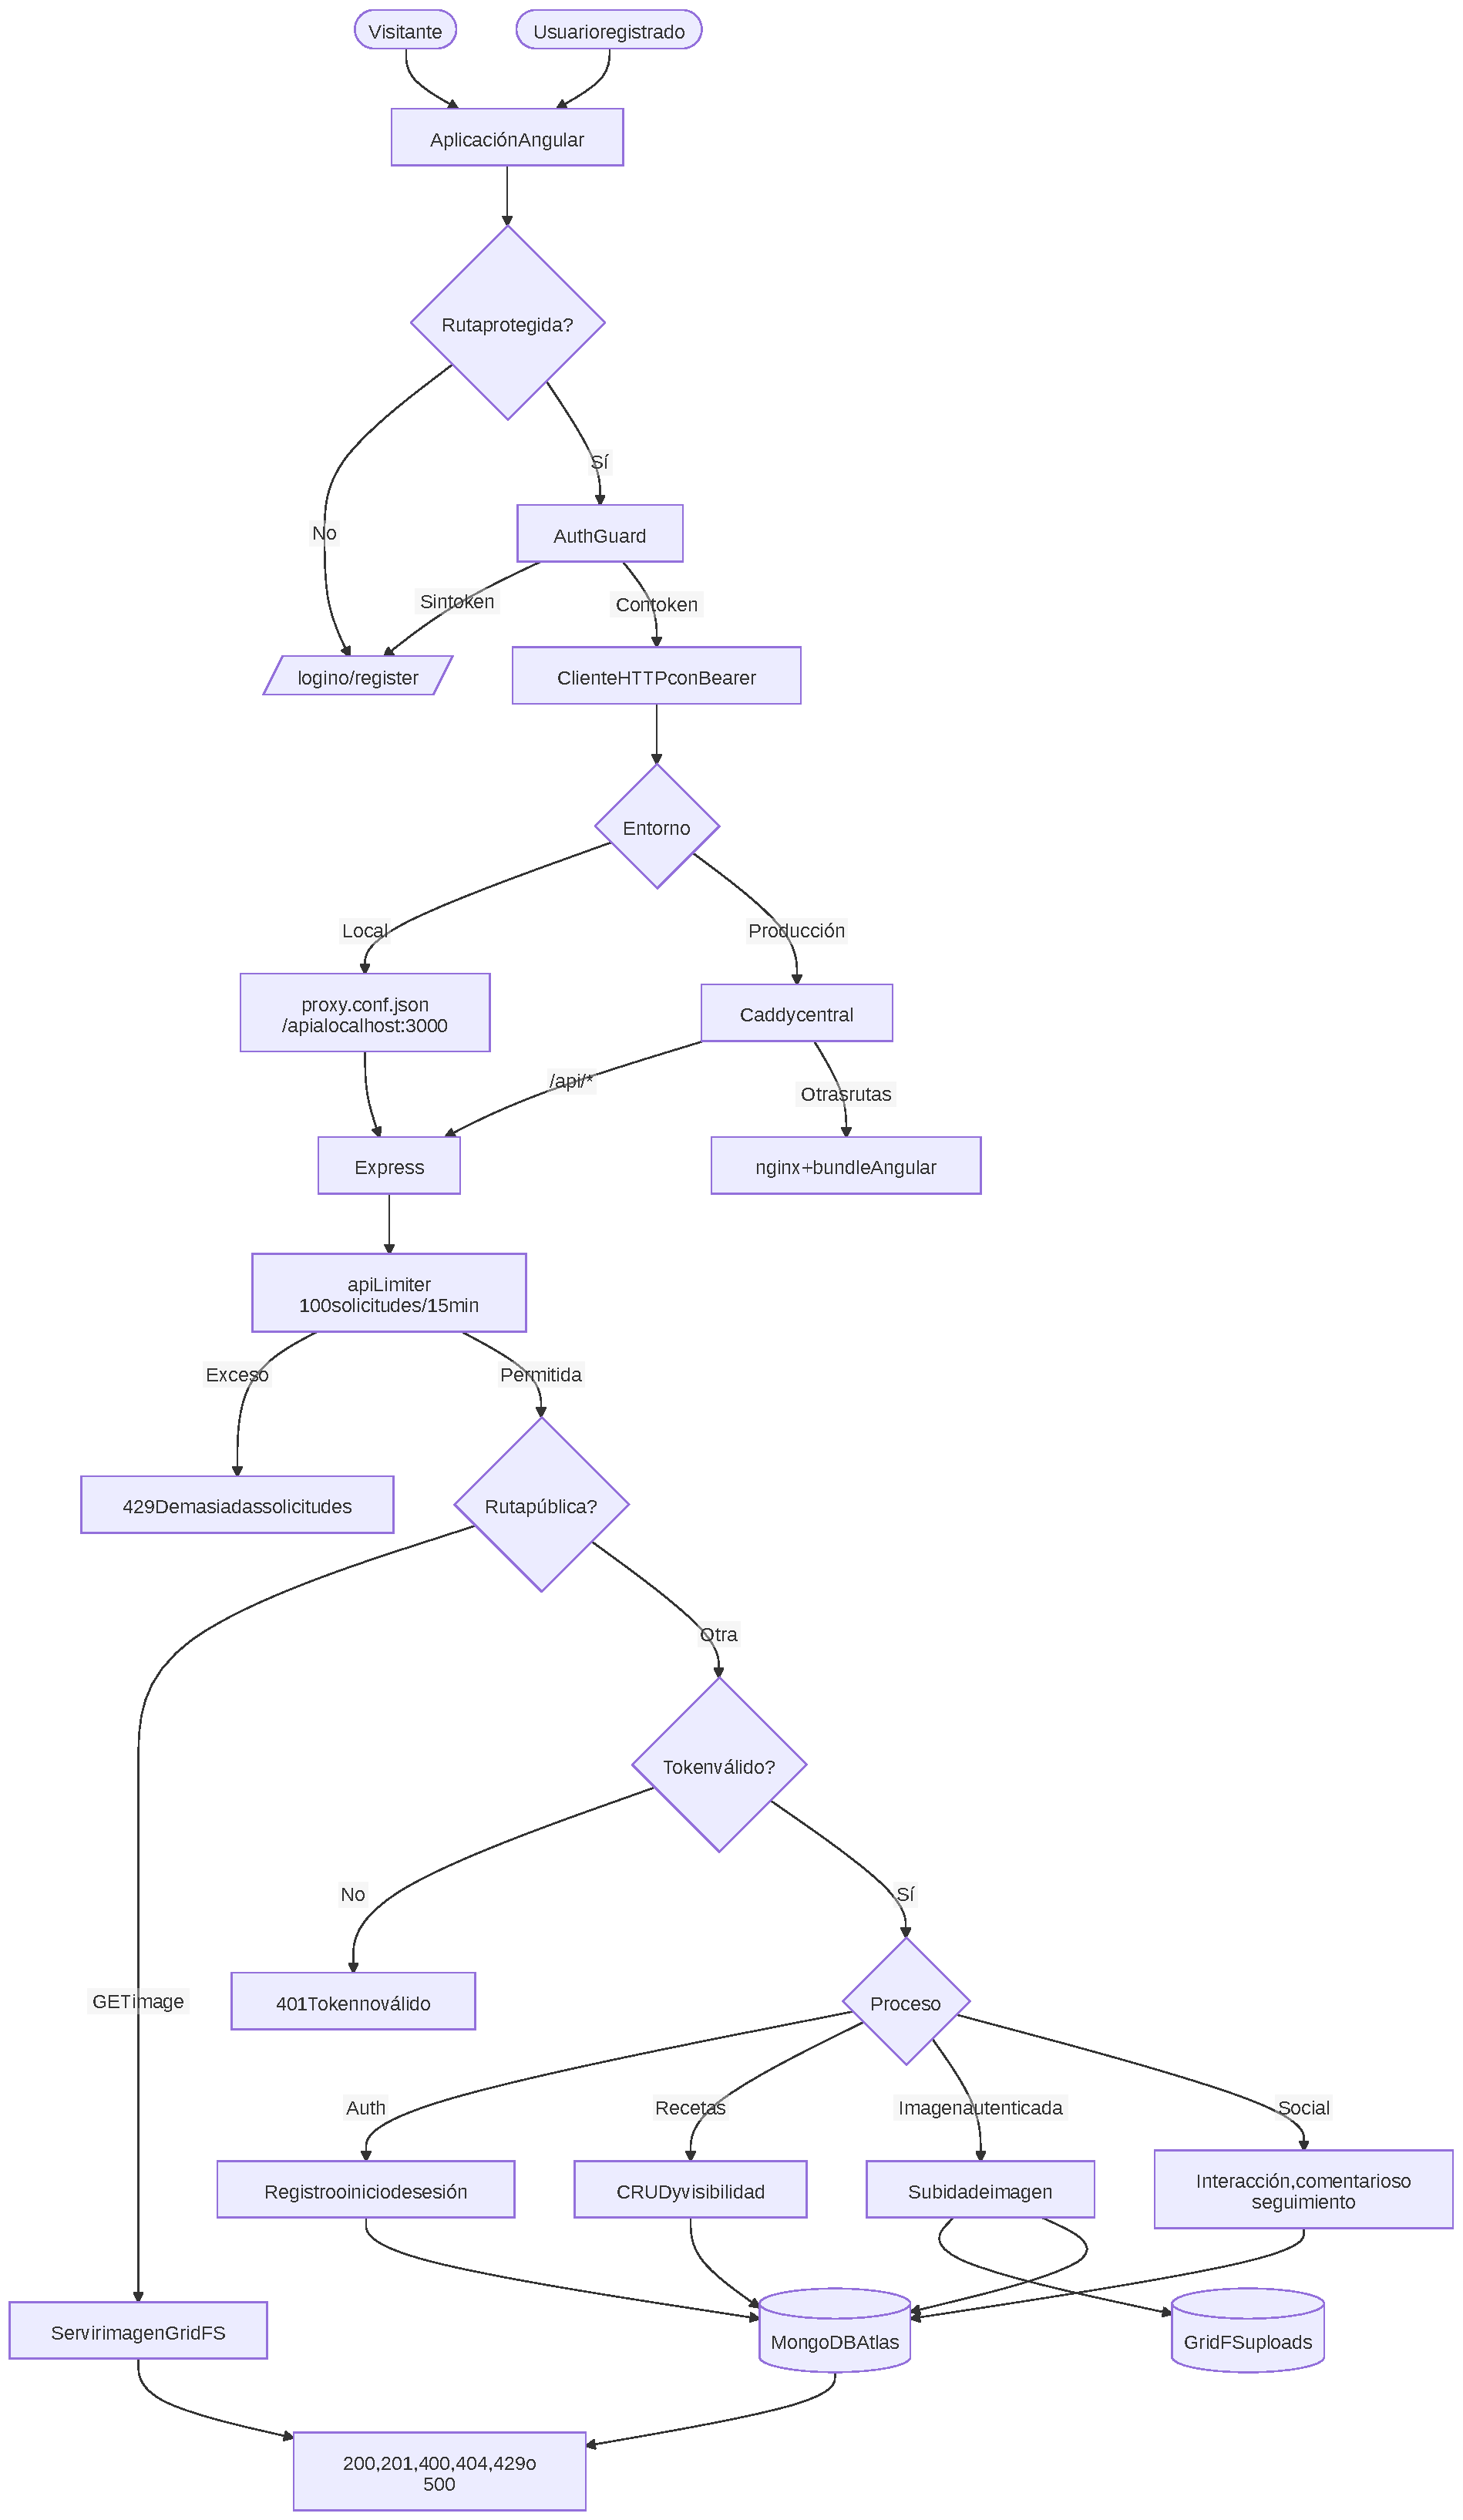
\includegraphics[width=0.72\textwidth, height=0.78\textheight, keepaspectratio]{figuras/flujo/flujo-sistema-general.pdf}
    \captionof{figure}{Diagrama de flujo general del sistema FoodLoop.}
    \label{fig:flujo-general}
\end{figure}

% =====================================================================
% 6. CASOS DE USO
% =====================================================================
\section{Casos de uso}

Los casos de uso describen las interacciones entre los actores y el sistema por cada proceso. Cada módulo incluye su diagrama y las fichas narrativas correspondientes.

\subsection{Casos de uso del módulo de autenticación}

\begin{figure}[H]
    \centering
    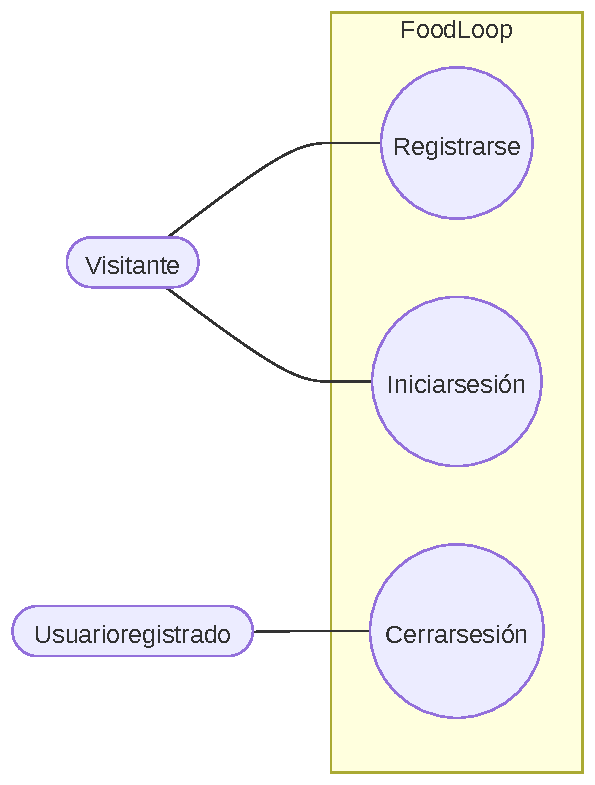
\includegraphics[width=0.72\textwidth, height=0.78\textheight, keepaspectratio]{figuras/casos-uso/casos-uso-autenticacion-y-sesion.pdf}
    \captionof{figure}{Diagrama de casos de uso de autenticación y sesión.}
    \label{fig:cu-autenticacion}
\end{figure}

\subsubsection{Caso de uso ``CU-01: Registrarse''}

\begin{longtable}{|P{3.3cm}|L{11.2cm}|}
\hline
\textbf{Descripción} & El visitante crea una cuenta con su nombre, correo y contraseña y recibe un token de sesión. \\ \hline
\textbf{Actores primarios} & Visitante. \\ \hline
\textbf{Contexto} & P01: Autenticación y sesión. \\ \hline
\textbf{Condiciones previas} & El correo no debe estar registrado. \\ \hline
\textbf{Flujo básico} &
\begin{enumerate}
    \item El visitante abre el formulario de registro.
    \item Ingresa su nombre, su correo y una contraseña de al menos 8 caracteres.
    \item El sistema sanea los campos y comprueba que el correo no exista.
    \item El sistema aplica el hash bcrypt a la contraseña y crea el usuario.
    \item El sistema emite un token JWT y lo devuelve al cliente.
\end{enumerate} \\ \hline
\textbf{Requerimientos especiales} & Contraseña de al menos 8 caracteres y correo único. \\ \hline
\textbf{Salida} & Usuario creado con respuesta \texttt{201} e ingreso al tablero. \\ \hline
\textbf{Excepciones} & Correo ya registrado (\texttt{400}); contraseña corta; exceso de intentos (\texttt{429}). \\ \hline
\end{longtable}

\subsubsection{Caso de uso ``CU-02: Iniciar sesión''}

\begin{longtable}{|P{3.3cm}|L{11.2cm}|}
\hline
\textbf{Descripción} & El usuario autenticado accede a la aplicación con sus credenciales. \\ \hline
\textbf{Actores primarios} & Visitante. \\ \hline
\textbf{Contexto} & P01: Autenticación y sesión. \\ \hline
\textbf{Condiciones previas} & El usuario debe estar registrado. \\ \hline
\textbf{Flujo básico} &
\begin{enumerate}
    \item El usuario ingresa su correo y su contraseña.
    \item El sistema busca el usuario y compara el hash de la contraseña.
    \item Si coinciden, el sistema emite un token JWT de 30 días.
    \item El cliente almacena el token y accede al tablero.
\end{enumerate} \\ \hline
\textbf{Requerimientos especiales} & Límite de 10 intentos cada 15 minutos. \\ \hline
\textbf{Salida} & Sesión iniciada con respuesta \texttt{200}. \\ \hline
\textbf{Excepciones} & Usuario o contraseña incorrectos (\texttt{400}); exceso de intentos (\texttt{429}). \\ \hline
\end{longtable}

\subsubsection{Caso de uso ``CU-03: Cerrar sesión''}

\begin{longtable}{|P{3.3cm}|L{11.2cm}|}
\hline
\textbf{Descripción} & El usuario registrado termina su sesión en el navegador. \\ \hline
\textbf{Actores primarios} & Usuario registrado. \\ \hline
\textbf{Contexto} & P01: Autenticación y sesión. \\ \hline
\textbf{Condiciones previas} & El usuario debe haber iniciado sesión. \\ \hline
\textbf{Flujo básico} &
\begin{enumerate}
    \item El usuario pulsa la opción de cerrar sesión.
    \item El cliente elimina el token local.
    \item El cliente redirige a la pantalla de inicio de sesión.
\end{enumerate} \\ \hline
\textbf{Requerimientos especiales} & El cierre de sesión no invalida el token en el servidor. \\ \hline
\textbf{Salida} & Sesión cerrada localmente. \\ \hline
\textbf{Excepciones} & Un token copiado sigue siendo válido hasta su expiración. \\ \hline
\end{longtable}

\subsection{Casos de uso del módulo de recetas}

\begin{figure}[H]
    \centering
    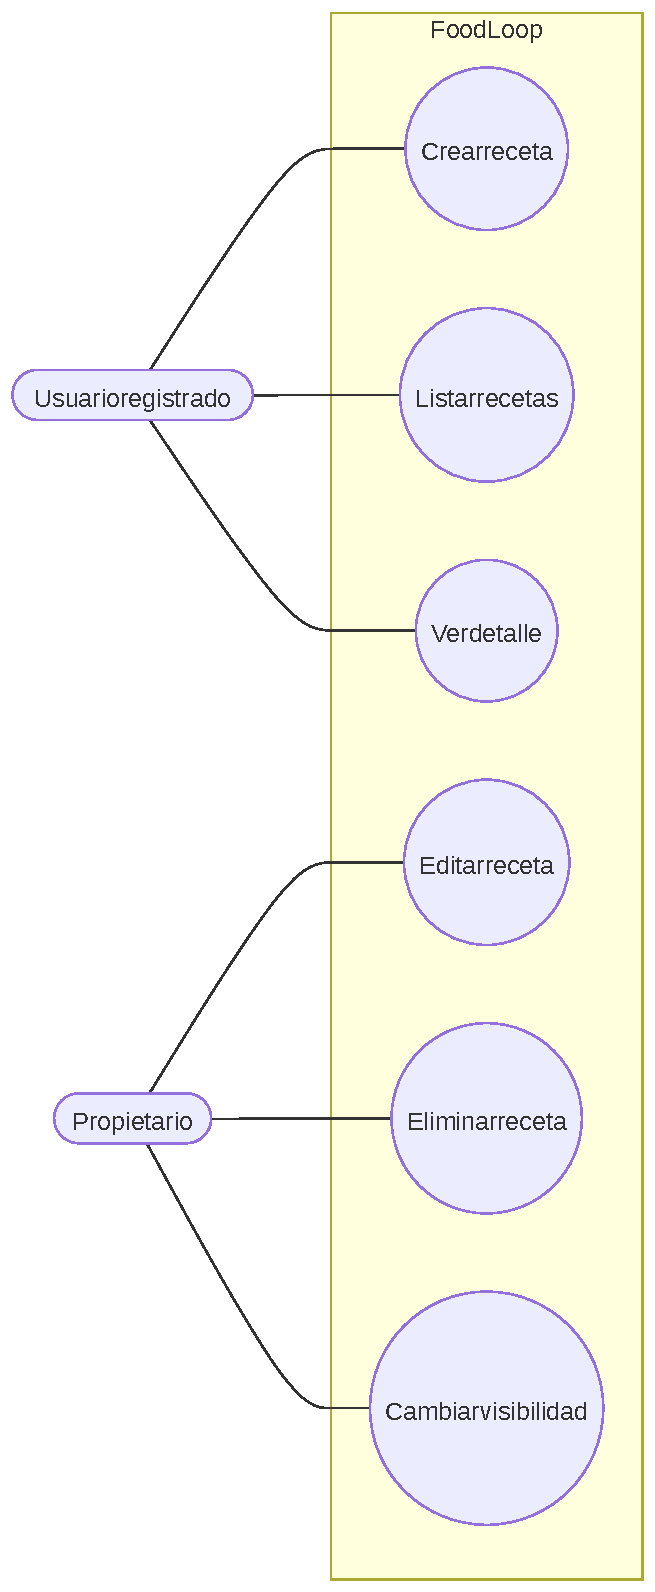
\includegraphics[width=0.72\textwidth, height=0.78\textheight, keepaspectratio]{figuras/casos-uso/casos-uso-recetas-y-visibilidad.pdf}
    \captionof{figure}{Diagrama de casos de uso de recetas y visibilidad.}
    \label{fig:cu-recetas}
\end{figure}

\subsubsection{Caso de uso ``CU-04: Crear receta''}

\begin{longtable}{|P{3.3cm}|L{11.2cm}|}
\hline
\textbf{Descripción} & El usuario guarda una receta propia. \\ \hline
\textbf{Actores primarios} & Usuario registrado. \\ \hline
\textbf{Contexto} & P02: Gestión de recetas y visibilidad. \\ \hline
\textbf{Condiciones previas} & El usuario debe tener una sesión válida. \\ \hline
\textbf{Flujo básico} &
\begin{enumerate}
    \item El usuario completa el formulario de receta.
    \item El sistema conserva únicamente los campos editables y asigna el propietario.
    \item La receta se guarda en estado privado.
    \item El sistema confirma la creación con la receta creada.
\end{enumerate} \\ \hline
\textbf{Requerimientos especiales} & Límite de 10 creaciones por minuto; la receta nace privada. \\ \hline
\textbf{Salida} & Receta creada con respuesta \texttt{201}. \\ \hline
\textbf{Excepciones} & Exceso de creaciones (\texttt{429}); error de validación. \\ \hline
\end{longtable}

\subsubsection{Caso de uso ``CU-05: Listar y ver recetas''}

\begin{longtable}{|P{3.3cm}|L{11.2cm}|}
\hline
\textbf{Descripción} & El usuario consulta sus recetas o las recetas públicas de otros usuarios. \\ \hline
\textbf{Actores primarios} & Usuario registrado. \\ \hline
\textbf{Contexto} & P02: Gestión de recetas y visibilidad. \\ \hline
\textbf{Condiciones previas} & El usuario debe tener una sesión válida. \\ \hline
\textbf{Flujo básico} &
\begin{enumerate}
    \item El tablero solicita las recetas propias o, con \texttt{scope=public}, las públicas.
    \item El sistema devuelve la lista correspondiente.
    \item Al abrir el detalle, el sistema permite la receta propia o una pública.
\end{enumerate} \\ \hline
\textbf{Requerimientos especiales} & Sin paginación ni búsqueda en el servidor. \\ \hline
\textbf{Salida} & Lista y detalle mostrados. \\ \hline
\textbf{Excepciones} & Receta privada ajena (\texttt{404}); identificador inválido puede producir error. \\ \hline
\end{longtable}

\subsubsection{Caso de uso ``CU-06: Editar, eliminar y cambiar visibilidad''}

\begin{longtable}{|P{3.3cm}|L{11.2cm}|}
\hline
\textbf{Descripción} & El propietario actualiza, borra o publica una receta. \\ \hline
\textbf{Actores primarios} & Propietario de receta. \\ \hline
\textbf{Contexto} & P02: Gestión de recetas y visibilidad. \\ \hline
\textbf{Condiciones previas} & El usuario debe ser propietario de la receta. \\ \hline
\textbf{Flujo básico} &
\begin{enumerate}
    \item El propietario guarda los cambios, confirma el borrado o alterna la visibilidad.
    \item El sistema valida la propiedad y aplica la lista de campos editables.
    \item El sistema ejecuta los validadores y persiste el cambio.
\end{enumerate} \\ \hline
\textbf{Requerimientos especiales} & El borrado es físico y deja huérfanos los comentarios, reseñas y actividades asociados. \\ \hline
\textbf{Salida} & Receta actualizada, eliminada o publicada. \\ \hline
\textbf{Excepciones} & Sin campos editables (\texttt{400}); receta ajena o inexistente (\texttt{404}). \\ \hline
\end{longtable}

\subsection{Casos de uso del módulo de imágenes}

\begin{figure}[H]
    \centering
    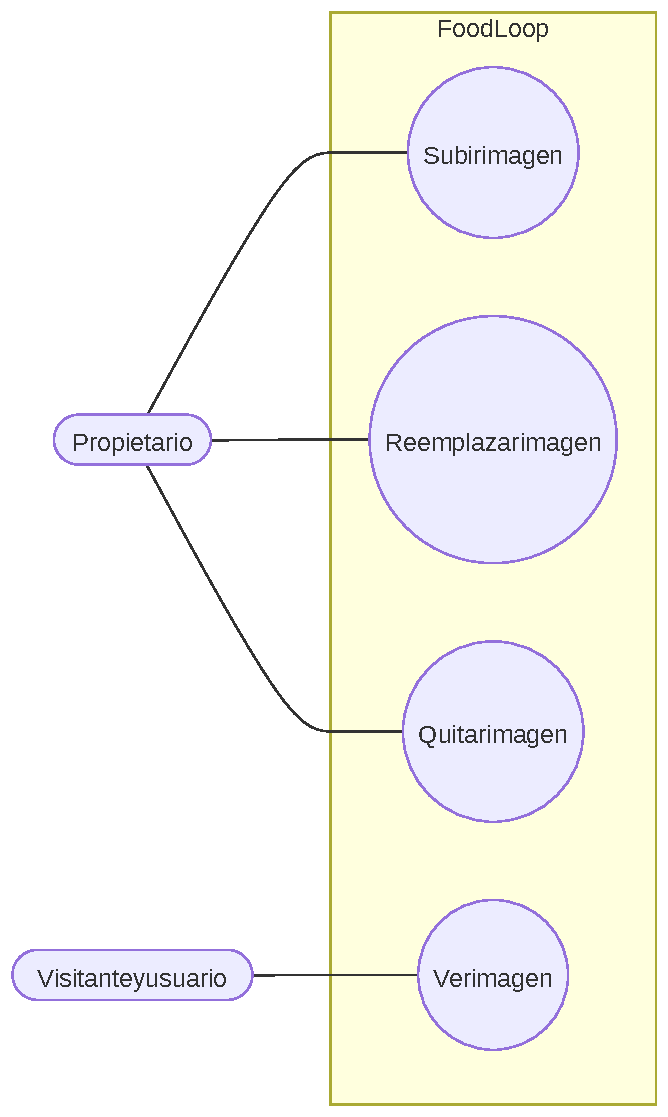
\includegraphics[width=0.72\textwidth, height=0.78\textheight, keepaspectratio]{figuras/casos-uso/casos-uso-imagenes.pdf}
    \captionof{figure}{Diagrama de casos de uso de imágenes.}
    \label{fig:cu-imagenes}
\end{figure}

\subsubsection{Caso de uso ``CU-07: Subir imagen''}

\begin{longtable}{|P{3.3cm}|L{11.2cm}|}
\hline
\textbf{Descripción} & El propietario asocia una imagen optimizada a una receta existente. \\ \hline
\textbf{Actores primarios} & Propietario de receta. \\ \hline
\textbf{Contexto} & P03: Gestión de imágenes. \\ \hline
\textbf{Condiciones previas} & La receta debe existir y pertenecer al usuario. \\ \hline
\textbf{Flujo básico} &
\begin{enumerate}
    \item El usuario selecciona un archivo de imagen.
    \item El navegador valida el tipo y optimiza la imagen a 1600 px y JPEG de calidad 0.8.
    \item El archivo se envía como \texttt{multipart/form-data}.
    \item El servidor guarda la imagen en GridFS, actualiza el identificador de la receta y elimina la imagen anterior.
\end{enumerate} \\ \hline
\textbf{Requerimientos especiales} & MIME de imagen, 25 MB en el navegador y 5 MB en el servidor. \\ \hline
\textbf{Salida} & Receta con imagen actualizada (\texttt{200}). \\ \hline
\textbf{Excepciones} & Tipo no permitido o tamaño excedido (\texttt{400}); receta ajena (\texttt{404}). \\ \hline
\end{longtable}

\subsubsection{Caso de uso ``CU-08: Reemplazar o quitar imagen''}

\begin{longtable}{|P{3.3cm}|L{11.2cm}|}
\hline
\textbf{Descripción} & El propietario mantiene una sola imagen vigente o deja la receta sin imagen. \\ \hline
\textbf{Actores primarios} & Propietario de receta. \\ \hline
\textbf{Contexto} & P03: Gestión de imágenes. \\ \hline
\textbf{Condiciones previas} & El usuario debe ser propietario de la receta. \\ \hline
\textbf{Flujo básico} &
\begin{enumerate}
    \item El propietario elige otra imagen o elimina la actual.
    \item El sistema registra el nuevo identificador o una cadena vacía.
    \item El sistema elimina de GridFS el archivo anterior.
\end{enumerate} \\ \hline
\textbf{Requerimientos especiales} & Solo se conserva una imagen vigente por receta. \\ \hline
\textbf{Salida} & Imagen reemplazada o eliminada. \\ \hline
\textbf{Excepciones} & Un fallo de subida conserva el identificador anterior. \\ \hline
\end{longtable}

\subsubsection{Caso de uso ``CU-09: Ver imagen''}

\begin{longtable}{|P{3.3cm}|L{11.2cm}|}
\hline
\textbf{Descripción} & El sistema muestra la imagen en tarjetas, detalle o enlace directo. \\ \hline
\textbf{Actores primarios} & Cualquier persona que conozca la URL pública. \\ \hline
\textbf{Contexto} & P03: Gestión de imágenes. \\ \hline
\textbf{Condiciones previas} & Se debe conocer el identificador del archivo. \\ \hline
\textbf{Flujo básico} &
\begin{enumerate}
    \item El cliente solicita la imagen por su identificador.
    \item El sistema valida el identificador y lee el archivo desde GridFS.
    \item El sistema devuelve el contenido con su tipo y aplica caché inmutable.
\end{enumerate} \\ \hline
\textbf{Requerimientos especiales} & Lectura pública, sin cabecera de autorización. \\ \hline
\textbf{Salida} & Imagen servida con respuesta \texttt{200}. \\ \hline
\textbf{Excepciones} & Identificador inválido (\texttt{400}); archivo inexistente (\texttt{404}). \\ \hline
\end{longtable}

\subsection{Casos de uso del módulo de interacciones sociales}

\begin{figure}[H]
    \centering
    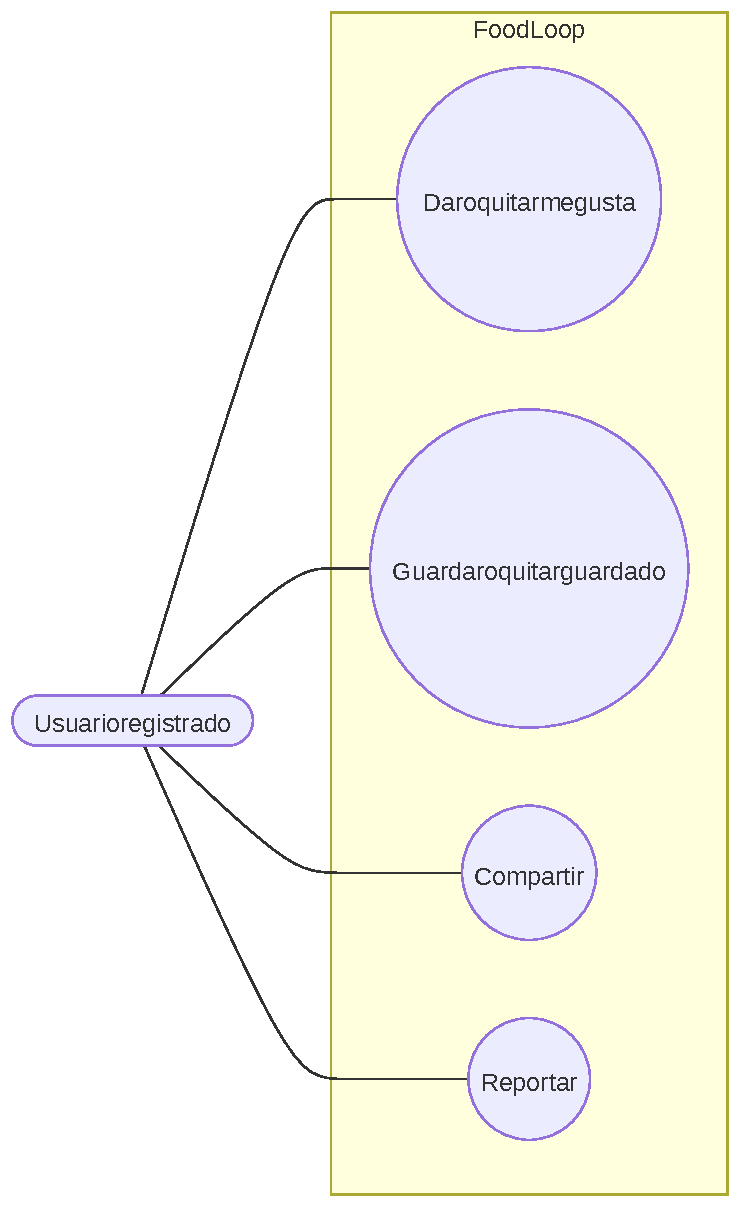
\includegraphics[width=0.72\textwidth, height=0.78\textheight, keepaspectratio]{figuras/casos-uso/casos-uso-interacciones-sociales.pdf}
    \captionof{figure}{Diagrama de casos de uso de interacciones sociales.}
    \label{fig:cu-interacciones}
\end{figure}

\subsubsection{Caso de uso ``CU-10: Me gusta''}

\begin{longtable}{|P{3.3cm}|L{11.2cm}|}
\hline
\textbf{Descripción} & El usuario marca o desmarca una receta con un me gusta. \\ \hline
\textbf{Actores primarios} & Usuario registrado. \\ \hline
\textbf{Contexto} & P04: Interacciones sociales. \\ \hline
\textbf{Condiciones previas} & El usuario debe tener una sesión válida. \\ \hline
\textbf{Flujo básico} &
\begin{enumerate}
    \item El usuario pulsa el corazón de una receta.
    \item El sistema alterna el estado del me gusta.
    \item El sistema sincroniza los favoritos del usuario y la receta, y registra la actividad para el autor.
\end{enumerate} \\ \hline
\textbf{Requerimientos especiales} & Límite social de 30 acciones por minuto. \\ \hline
\textbf{Salida} & Estado alternado con \texttt{liked} y \texttt{likesCount}. \\ \hline
\textbf{Excepciones} & Receta inexistente (\texttt{404}); la API no impide el me gusta propio. \\ \hline
\end{longtable}

\subsubsection{Caso de uso ``CU-10b: Guardar receta''}

\begin{longtable}{|P{3.3cm}|L{11.2cm}|}
\hline
\textbf{Descripción} & El usuario guarda o quita una receta de su lista de guardados. \\ \hline
\textbf{Actores primarios} & Usuario registrado. \\ \hline
\textbf{Contexto} & P04: Interacciones sociales. \\ \hline
\textbf{Condiciones previas} & El usuario debe tener una sesión válida. \\ \hline
\textbf{Flujo básico} &
\begin{enumerate}
    \item El usuario pulsa el botón de guardar.
    \item El sistema alterna el estado y actualiza el contador de guardados de la receta.
\end{enumerate} \\ \hline
\textbf{Requerimientos especiales} & La operación no sincroniza los favoritos del usuario. \\ \hline
\textbf{Salida} & Estado alternado con \texttt{saved} y \texttt{guardadosCount}. \\ \hline
\textbf{Excepciones} & Receta inexistente (\texttt{404}). \\ \hline
\end{longtable}

\subsubsection{Caso de uso ``CU-10c: Compartir receta''}

\begin{longtable}{|P{3.3cm}|L{11.2cm}|}
\hline
\textbf{Descripción} & El usuario comparte una receta, lo que incrementa su contador de compartidos. \\ \hline
\textbf{Actores primarios} & Usuario registrado. \\ \hline
\textbf{Contexto} & P04: Interacciones sociales. \\ \hline
\textbf{Condiciones previas} & El usuario debe tener una sesión válida. \\ \hline
\textbf{Flujo básico} &
\begin{enumerate}
    \item El usuario pulsa la opción de compartir.
    \item El sistema incrementa el contador de compartidos e intenta registrar la actividad.
\end{enumerate} \\ \hline
\textbf{Requerimientos especiales} & Defecto conocido: el tipo \texttt{compartio\_receta} no está en la enumeración de actividad y la operación puede fallar. \\ \hline
\textbf{Salida} & Contador incrementado. \\ \hline
\textbf{Excepciones} & Puede devolver \texttt{500} después de incrementar el contador. \\ \hline
\end{longtable}

\subsubsection{Caso de uso ``CU-10d: Reportar receta''}

\begin{longtable}{|P{3.3cm}|L{11.2cm}|}
\hline
\textbf{Descripción} & El usuario informa contenido inapropiado indicando un motivo. \\ \hline
\textbf{Actores primarios} & Usuario registrado. \\ \hline
\textbf{Contexto} & P04: Interacciones sociales. \\ \hline
\textbf{Condiciones previas} & El usuario debe tener una sesión válida. \\ \hline
\textbf{Flujo básico} &
\begin{enumerate}
    \item El usuario envía un motivo de reporte.
    \item El sistema sanea el motivo, guarda el reporte y marca la receta como reportada.
\end{enumerate} \\ \hline
\textbf{Requerimientos especiales} & Admite reportes repetidos; no existe moderación ni cuenta administradora. \\ \hline
\textbf{Salida} & Receta marcada como reportada. \\ \hline
\textbf{Excepciones} & Receta inexistente (\texttt{404}). \\ \hline
\end{longtable}

\subsection{Casos de uso del módulo de comentarios y reseñas}

\begin{figure}[H]
    \centering
    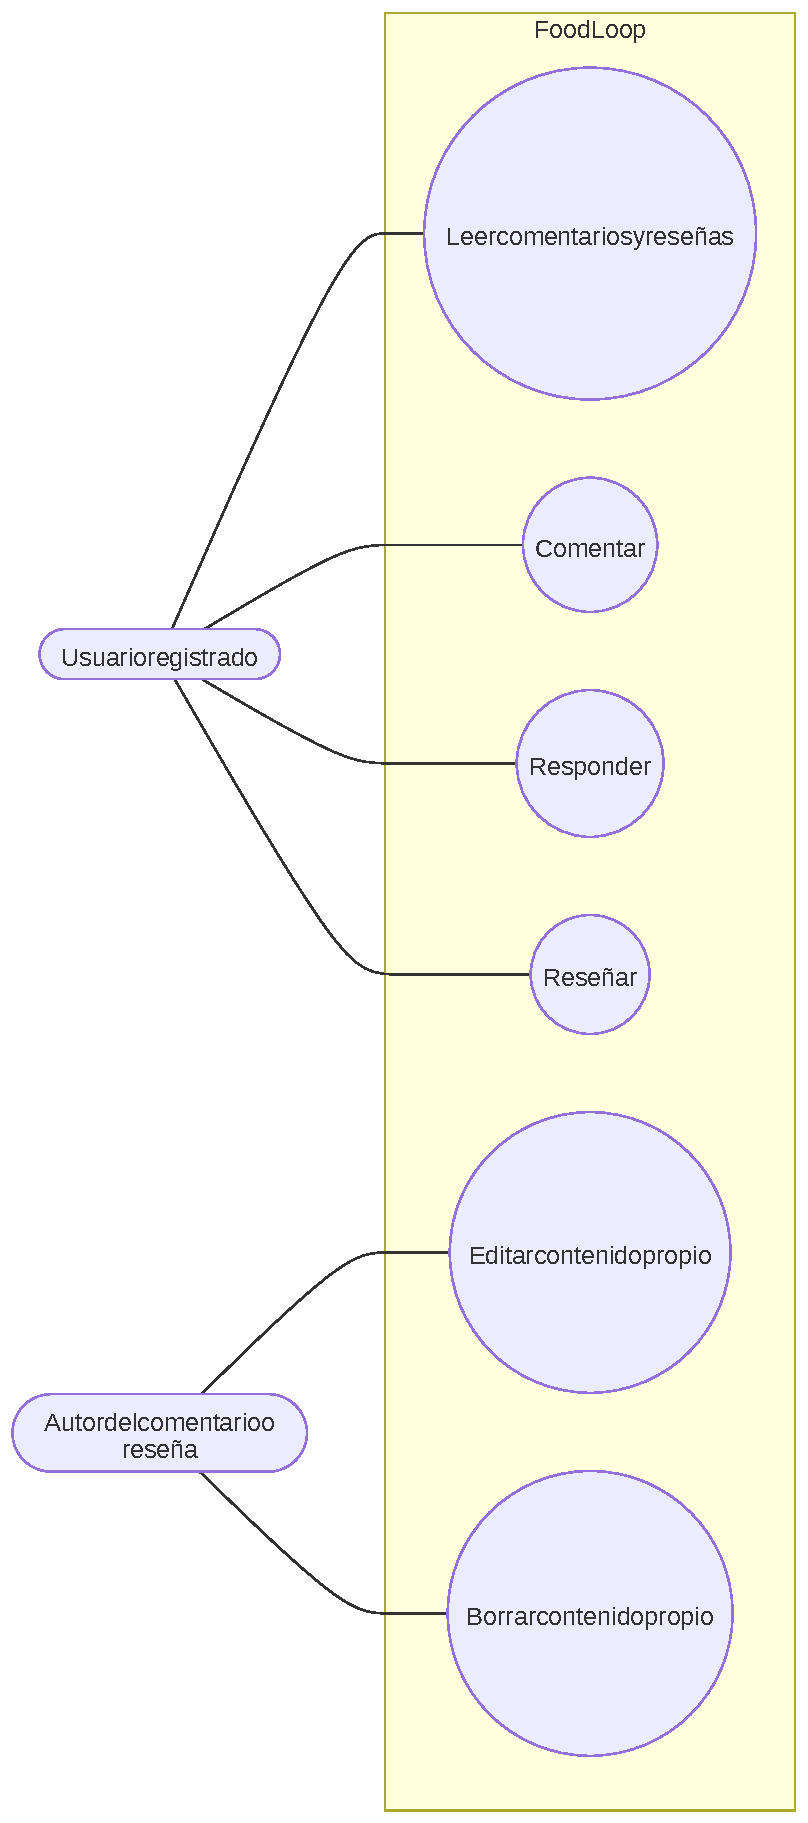
\includegraphics[width=0.72\textwidth, height=0.78\textheight, keepaspectratio]{figuras/casos-uso/casos-uso-comentarios-y-resenas.pdf}
    \captionof{figure}{Diagrama de casos de uso de comentarios y reseñas.}
    \label{fig:cu-comentarios}
\end{figure}

\subsubsection{Caso de uso ``CU-11: Leer comentarios y reseñas''}

\begin{longtable}{|P{3.3cm}|L{11.2cm}|}
\hline
\textbf{Descripción} & El usuario consulta la conversación y la calificación de una receta. \\ \hline
\textbf{Actores primarios} & Usuario registrado. \\ \hline
\textbf{Contexto} & P05: Comentarios y reseñas. \\ \hline
\textbf{Condiciones previas} & El usuario debe tener una sesión válida. \\ \hline
\textbf{Flujo básico} &
\begin{enumerate}
    \item El usuario abre el detalle de la receta.
    \item El sistema solicita los comentarios principales con un nivel de respuestas y las reseñas ordenadas.
    \item El sistema muestra los comentarios, las reseñas y el promedio de calificación.
\end{enumerate} \\ \hline
\textbf{Requerimientos especiales} & La lectura expone solo un nivel de respuestas. \\ \hline
\textbf{Salida} & Comentarios, reseñas y promedio mostrados. \\ \hline
\textbf{Excepciones} & Los errores de lectura muestran mensajes genéricos. \\ \hline
\end{longtable}

\subsubsection{Caso de uso ``CU-12: Comentar y responder''}

\begin{longtable}{|P{3.3cm}|L{11.2cm}|}
\hline
\textbf{Descripción} & El usuario publica un comentario o una respuesta de primer nivel. \\ \hline
\textbf{Actores primarios} & Usuario registrado. \\ \hline
\textbf{Contexto} & P05: Comentarios y reseñas. \\ \hline
\textbf{Condiciones previas} & Sesión válida y texto no vacío. \\ \hline
\textbf{Flujo básico} &
\begin{enumerate}
    \item El usuario escribe el comentario o la respuesta.
    \item El sistema lo guarda, incrementa el contador de la receta y registra la actividad.
    \item El comentario se muestra en el detalle.
\end{enumerate} \\ \hline
\textbf{Requerimientos especiales} & Límite de 10 creaciones por minuto; el borrado es lógico. \\ \hline
\textbf{Salida} & Comentario creado con respuesta \texttt{201}. \\ \hline
\textbf{Excepciones} & Texto vacío o excesivo; no se comprueba que la receta exista o sea visible. \\ \hline
\end{longtable}

\subsubsection{Caso de uso ``CU-13: Reseñar''}

\begin{longtable}{|P{3.3cm}|L{11.2cm}|}
\hline
\textbf{Descripción} & El usuario califica una receta de 1 a 5 estrellas, con un texto opcional. \\ \hline
\textbf{Actores primarios} & Usuario registrado. \\ \hline
\textbf{Contexto} & P05: Comentarios y reseñas. \\ \hline
\textbf{Condiciones previas} & Sesión válida y puntuación distinta de cero. \\ \hline
\textbf{Flujo básico} &
\begin{enumerate}
    \item El usuario envía su calificación y, opcionalmente, un texto.
    \item El sistema guarda la reseña y recalcula el promedio y el total de la receta.
    \item El sistema registra la actividad y muestra la reseña.
\end{enumerate} \\ \hline
\textbf{Requerimientos especiales} & Una sola reseña por usuario y receta; promedio redondeado a un decimal. \\ \hline
\textbf{Salida} & Reseña creada con respuesta \texttt{201} y promedio actualizado. \\ \hline
\textbf{Excepciones} & Segunda reseña del mismo usuario (\texttt{400}); puntuación inválida puede producir \texttt{500}. \\ \hline
\end{longtable}

\subsubsection{Caso de uso ``CU-14: Editar o borrar contenido propio''}

\begin{longtable}{|P{3.3cm}|L{11.2cm}|}
\hline
\textbf{Descripción} & El autor corrige o retira su propio comentario o reseña. \\ \hline
\textbf{Actores primarios} & Autor del contenido. \\ \hline
\textbf{Contexto} & P05: Comentarios y reseñas. \\ \hline
\textbf{Condiciones previas} & El usuario debe ser el autor del contenido. \\ \hline
\textbf{Flujo básico} &
\begin{enumerate}
    \item El autor actualiza el texto o solicita el borrado lógico.
    \item El sistema verifica la autoría y recalcula las métricas.
\end{enumerate} \\ \hline
\textbf{Requerimientos especiales} & La operación existe en la API, pero aún no tiene botones en la interfaz. \\ \hline
\textbf{Salida} & Comentario o reseña actualizado o retirado. \\ \hline
\textbf{Excepciones} & Control de autor; recurso inexistente (\texttt{404}). \\ \hline
\end{longtable}

\subsection{Casos de uso del módulo de seguimiento, feed y notificaciones}

\begin{figure}[H]
    \centering
    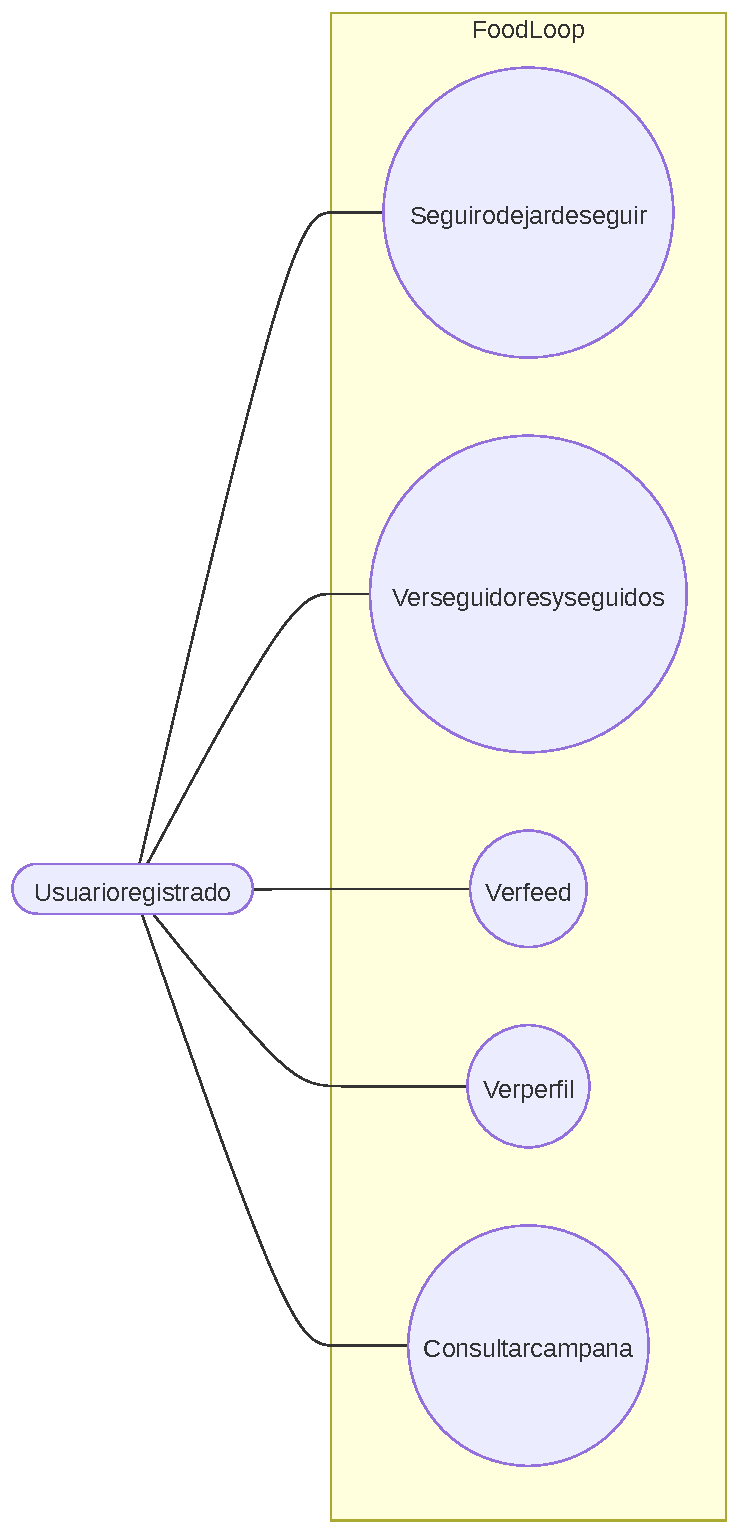
\includegraphics[width=0.72\textwidth, height=0.78\textheight, keepaspectratio]{figuras/casos-uso/casos-uso-seguimiento-feed-y-notificaciones.pdf}
    \captionof{figure}{Diagrama de casos de uso de seguimiento, feed y notificaciones.}
    \label{fig:cu-seguimiento}
\end{figure}

\subsubsection{Caso de uso ``CU-14b: Seguir o dejar de seguir''}

\begin{longtable}{|P{3.3cm}|L{11.2cm}|}
\hline
\textbf{Descripción} & El usuario se suscribe o cancela la suscripción a otro usuario. \\ \hline
\textbf{Actores primarios} & Usuario registrado. \\ \hline
\textbf{Contexto} & P06: Seguimiento, feed y notificaciones. \\ \hline
\textbf{Condiciones previas} & Sesión válida y un destinatario distinto del propio usuario. \\ \hline
\textbf{Flujo básico} &
\begin{enumerate}
    \item El usuario pulsa el botón de seguir en el perfil de otro usuario.
    \item El sistema alterna el documento de seguimiento.
    \item El sistema actualiza los contadores de seguidores y seguidos y registra la actividad.
\end{enumerate} \\ \hline
\textbf{Requerimientos especiales} & Pareja única de seguimiento; límite de 10 creaciones por minuto. \\ \hline
\textbf{Salida} & Estado alternado con \texttt{isFollowing}. \\ \hline
\textbf{Excepciones} & El usuario intenta seguirse a sí mismo (\texttt{400}). \\ \hline
\end{longtable}

\subsubsection{Caso de uso ``CU-15: Ver seguidores, seguidos y feed''}

\begin{longtable}{|P{3.3cm}|L{11.2cm}|}
\hline
\textbf{Descripción} & El usuario explora sus relaciones sociales y la actividad de las personas que sigue. \\ \hline
\textbf{Actores primarios} & Usuario registrado. \\ \hline
\textbf{Contexto} & P06: Seguimiento, feed y notificaciones. \\ \hline
\textbf{Condiciones previas} & El usuario debe tener una sesión válida. \\ \hline
\textbf{Flujo básico} &
\begin{enumerate}
    \item El usuario abre su perfil o su feed.
    \item El sistema devuelve los seguidores, los seguidos y las actividades paginadas.
    \item El sistema muestra las listas y el feed.
\end{enumerate} \\ \hline
\textbf{Requerimientos especiales} & Defecto conocido: \texttt{/profile/:username} envía un nombre donde el backend espera un identificador. \\ \hline
\textbf{Salida} & Listas y feed mostrados. \\ \hline
\textbf{Excepciones} & El perfil no resuelve correctamente el usuario, sus recetas ni su seguimiento. \\ \hline
\end{longtable}

\subsubsection{Caso de uso ``CU-16: Consultar la campana de notificaciones''}

\begin{longtable}{|P{3.3cm}|L{11.2cm}|}
\hline
\textbf{Descripción} & El usuario consulta la campana de notificaciones con la actividad reciente. \\ \hline
\textbf{Actores primarios} & Usuario registrado. \\ \hline
\textbf{Contexto} & P06: Seguimiento, feed y notificaciones. \\ \hline
\textbf{Condiciones previas} & El usuario debe tener una sesión válida. \\ \hline
\textbf{Flujo básico} &
\begin{enumerate}
    \item El usuario abre la campana de notificaciones.
    \item El sistema reutiliza las actividades del feed y descarta las propias.
    \item El sistema muestra las notificaciones y su contador.
\end{enumerate} \\ \hline
\textbf{Requerimientos especiales} & La campana no persiste el estado leído y cuenta todas las actividades como nuevas. \\ \hline
\textbf{Salida} & Campana de notificaciones mostrada. \\ \hline
\textbf{Excepciones} & Pendiente la persistencia de notificaciones (prevista para un ciclo posterior). \\ \hline
\end{longtable}

% =====================================================================
% 7. DIAGRAMA DE SECUENCIA
% =====================================================================
\section{Diagrama de secuencia}

Los diagramas de secuencia muestran el intercambio de mensajes entre los componentes en los procesos con mayor interacción. Las fuentes editables se encuentran en el directorio \texttt{docs/diagramas/secuencia}.

\subsection{Secuencia de registro e inicio de sesión}

\begin{figure}[H]
    \centering
    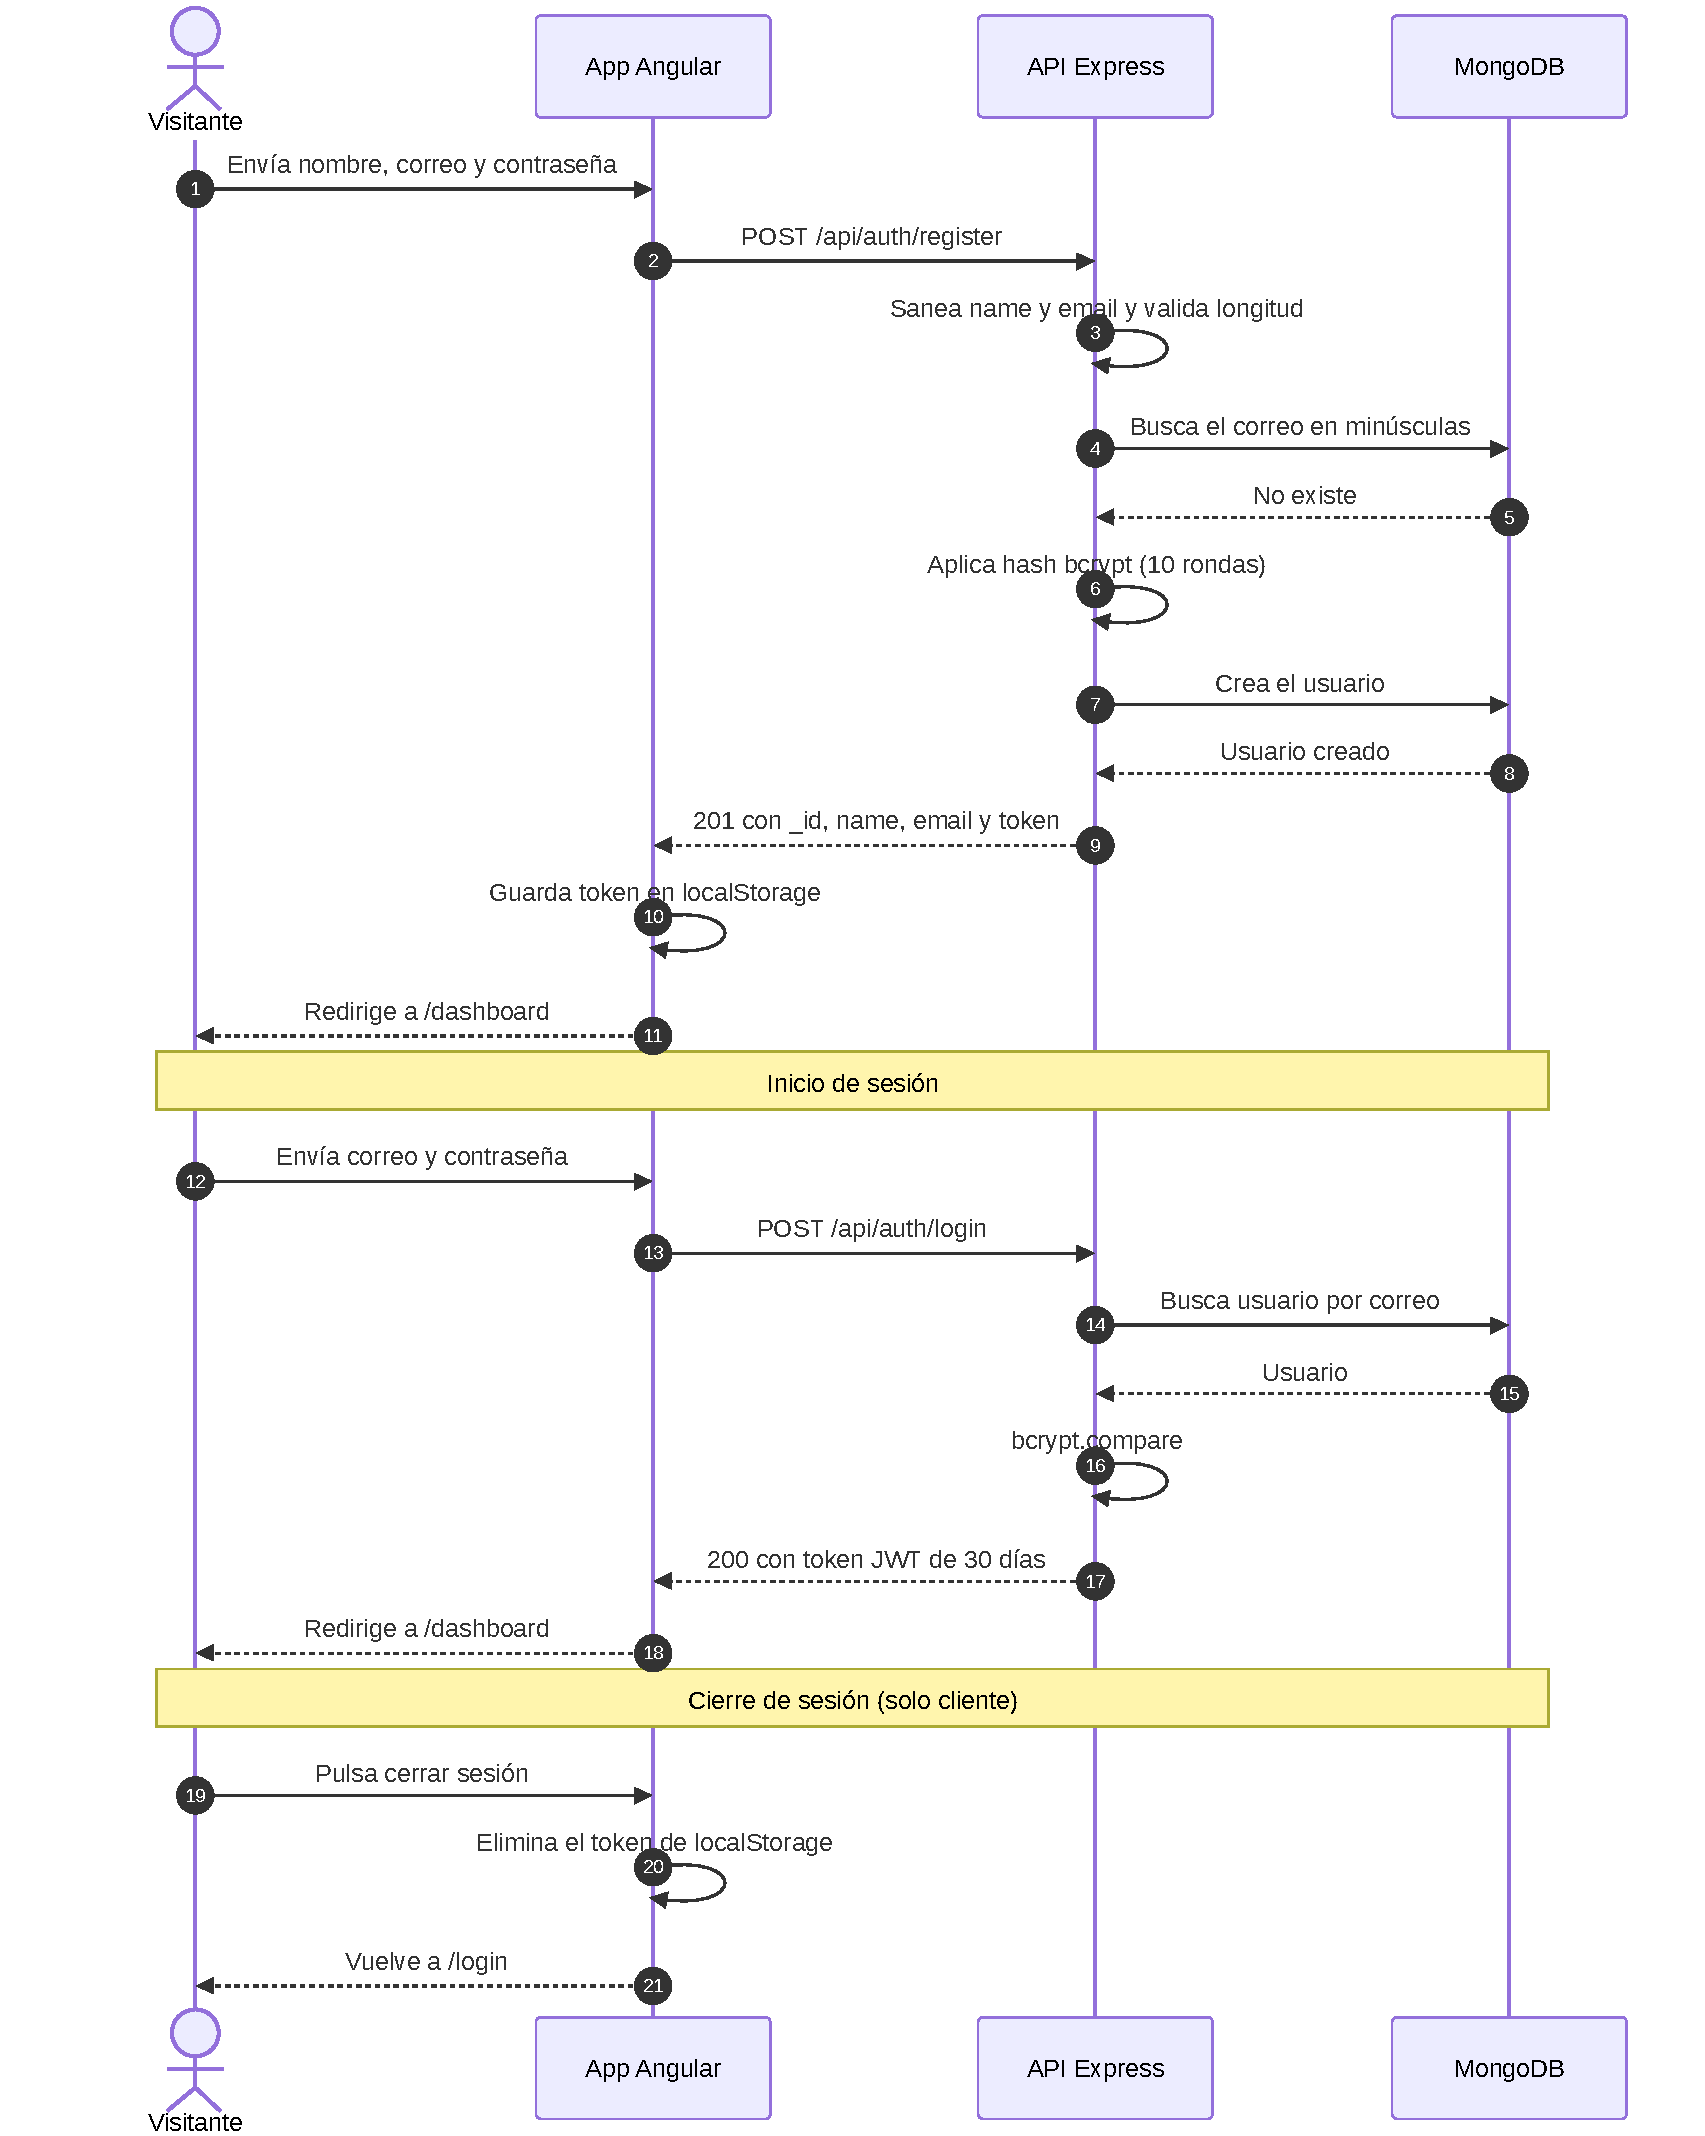
\includegraphics[width=0.72\textwidth, height=0.78\textheight, keepaspectratio]{figuras/secuencia/secuencia-registro-e-inicio-sesion.pdf}
    \captionof{figure}{Secuencia de registro e inicio de sesión.}
    \label{fig:sec-login}
\end{figure}

\subsection{Secuencia de creación de receta y gestión de imagen}

\begin{figure}[H]
    \centering
    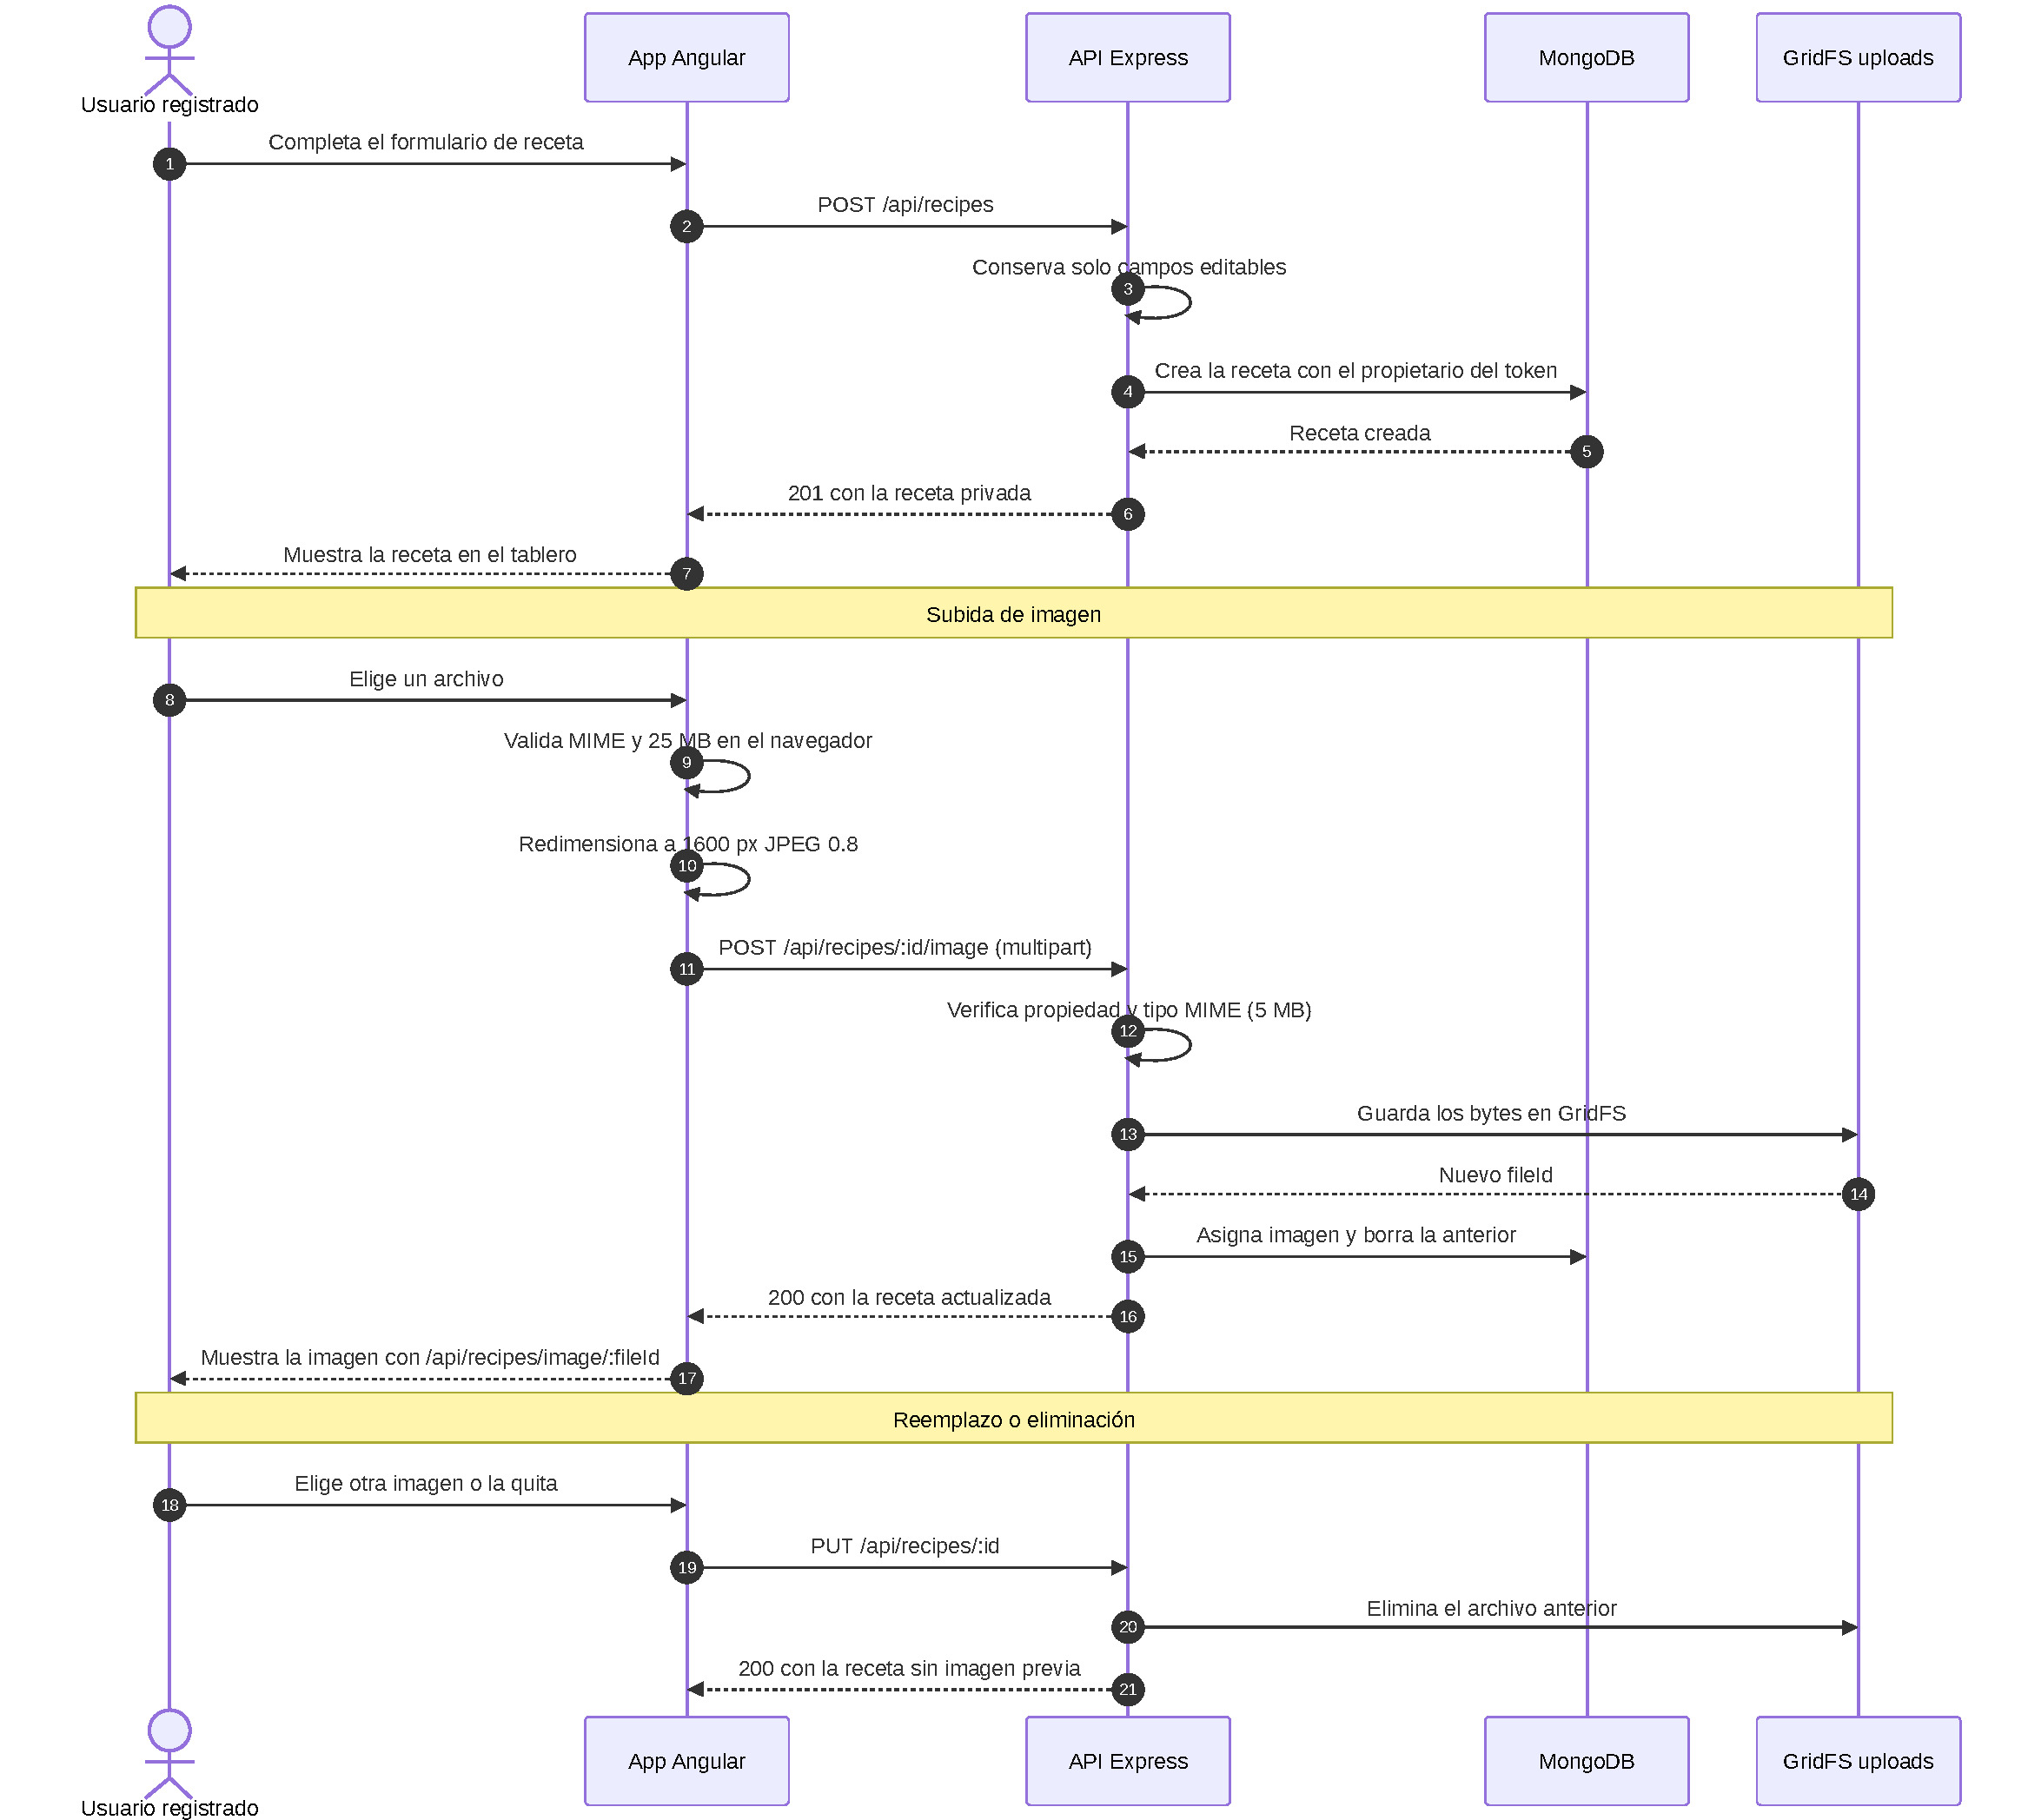
\includegraphics[width=0.72\textwidth, height=0.78\textheight, keepaspectratio]{figuras/secuencia/secuencia-crear-receta-y-gestionar-imagen.pdf}
    \captionof{figure}{Secuencia de creación de una receta y subida de su imagen.}
    \label{fig:sec-receta}
\end{figure}

\subsection{Secuencia de comentar y reseñar}

\begin{figure}[H]
    \centering
    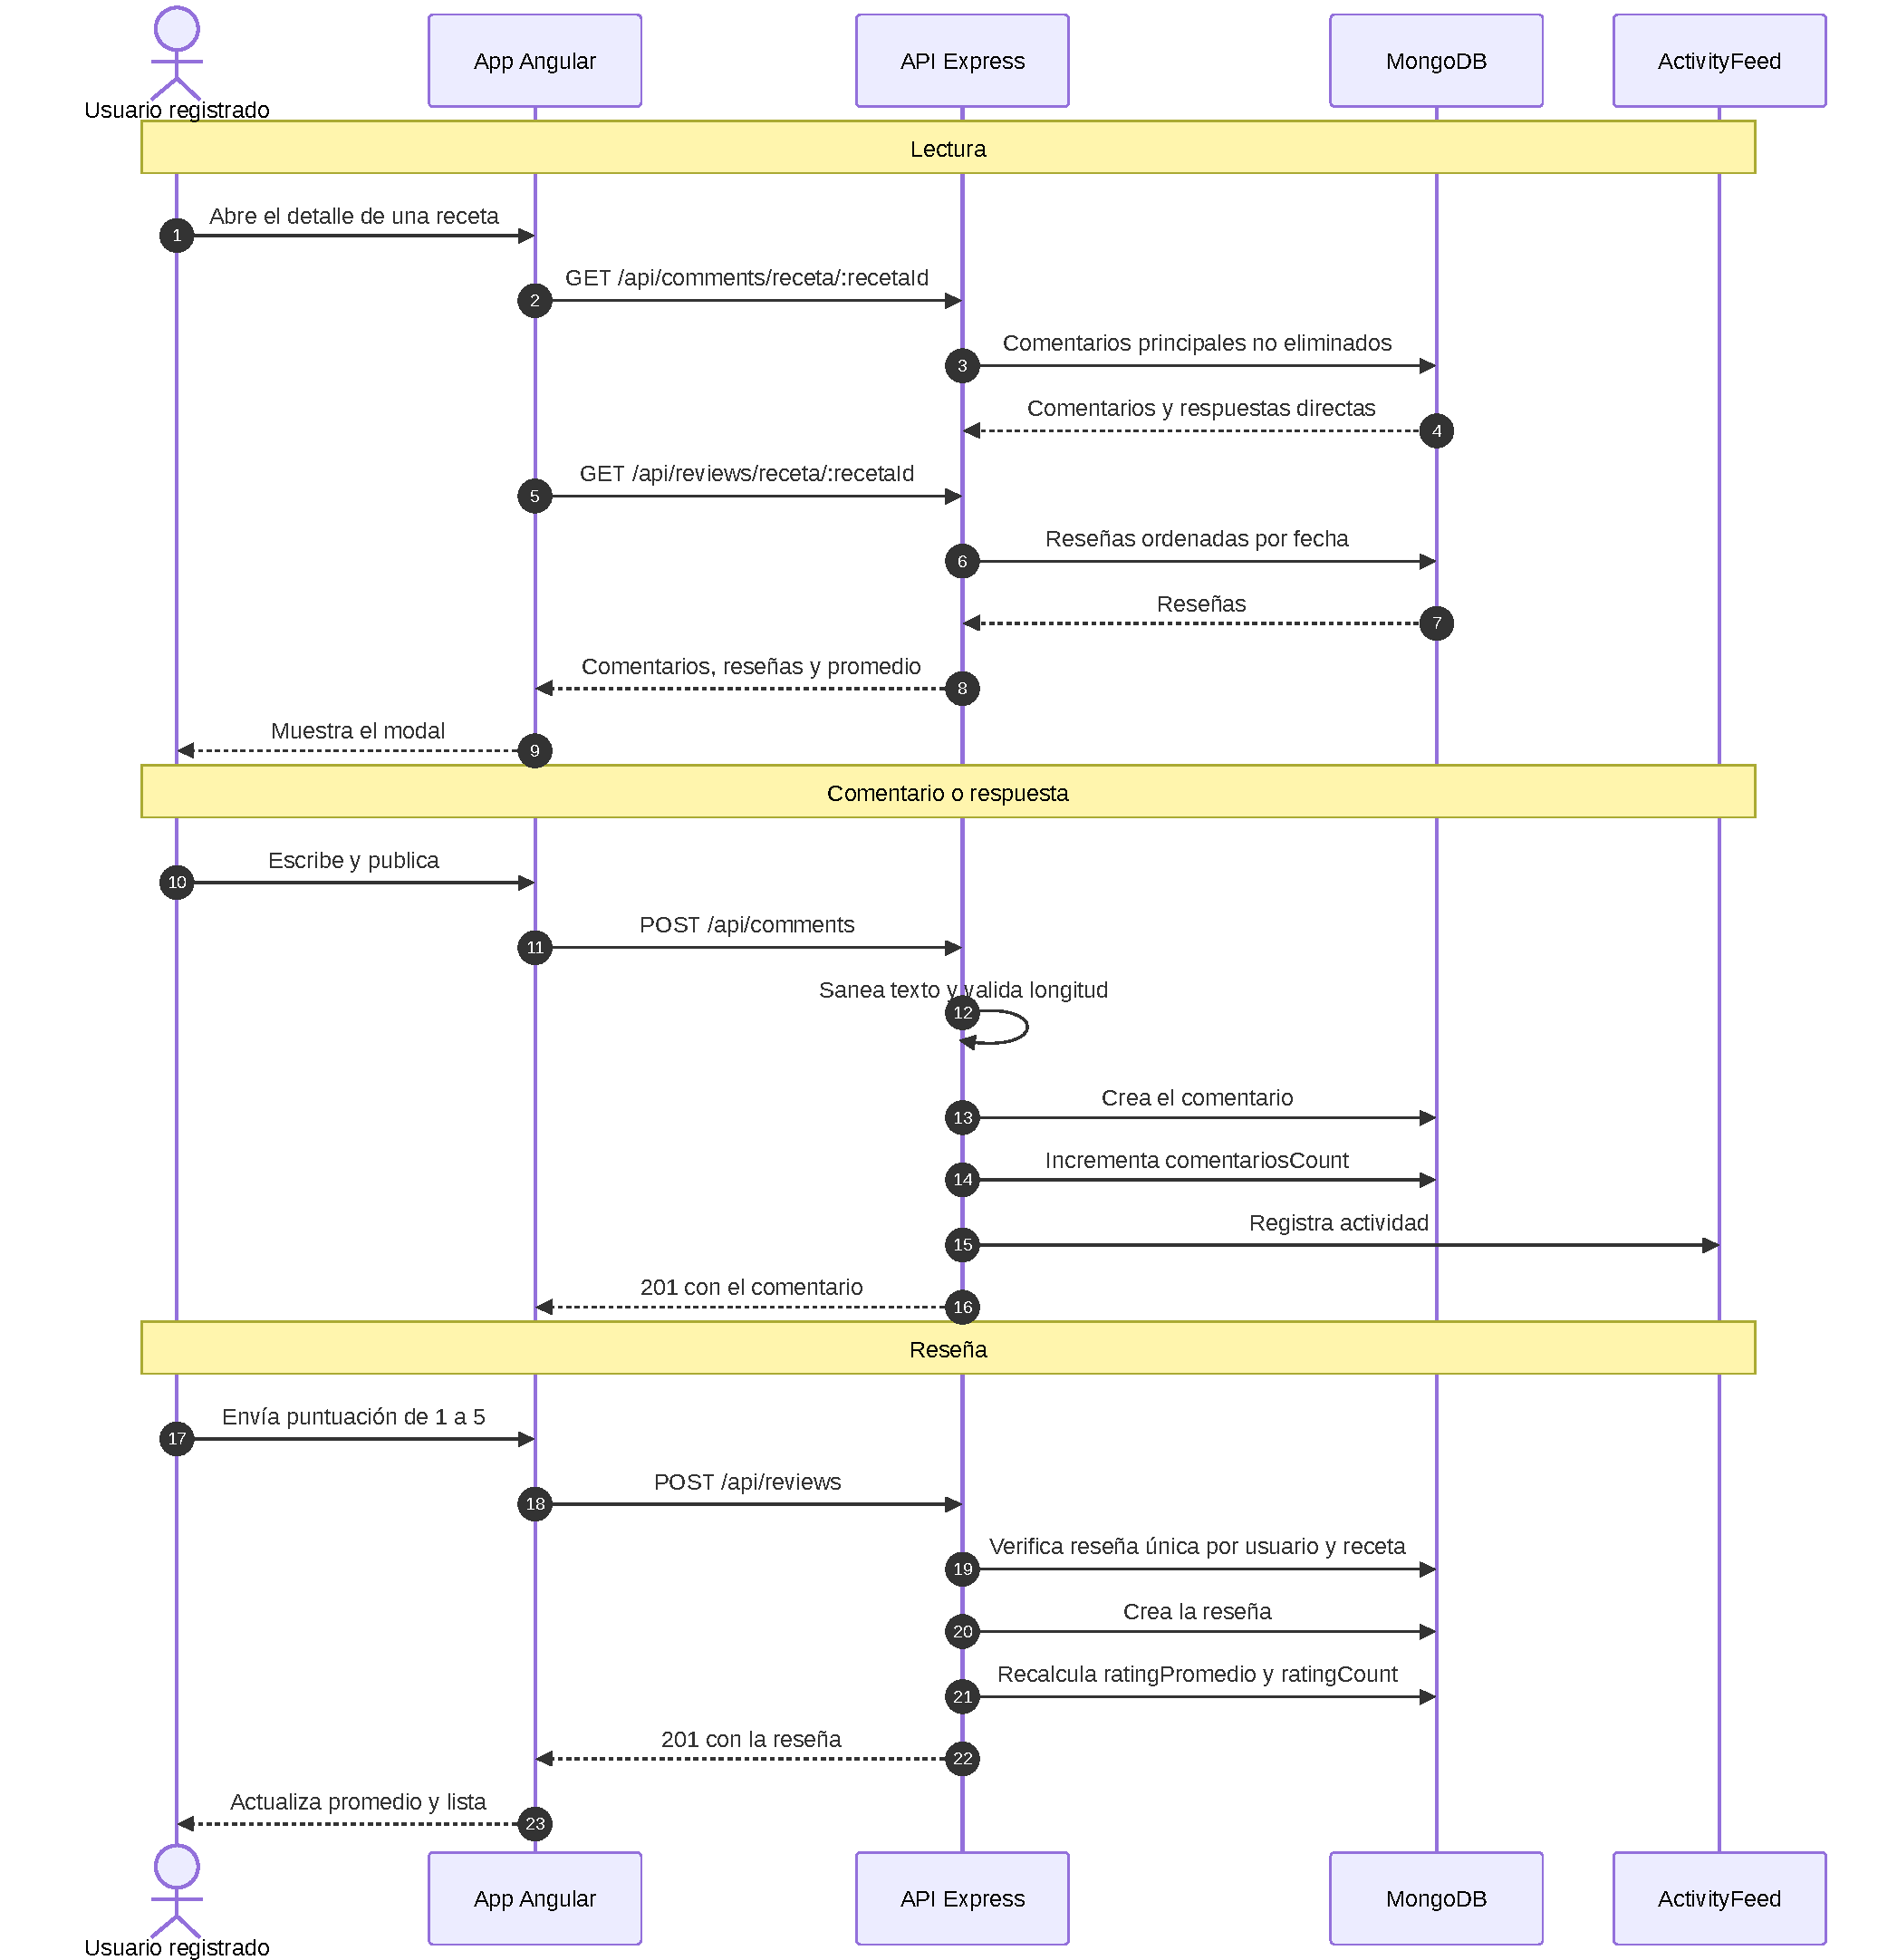
\includegraphics[width=0.72\textwidth, height=0.78\textheight, keepaspectratio]{figuras/secuencia/secuencia-comentar-y-resenar.pdf}
    \captionof{figure}{Secuencia de publicación de un comentario y de una reseña.}
    \label{fig:sec-comentario}
\end{figure}

\subsection{Secuencia de seguir usuarios y consultar el feed}

\begin{figure}[H]
    \centering
    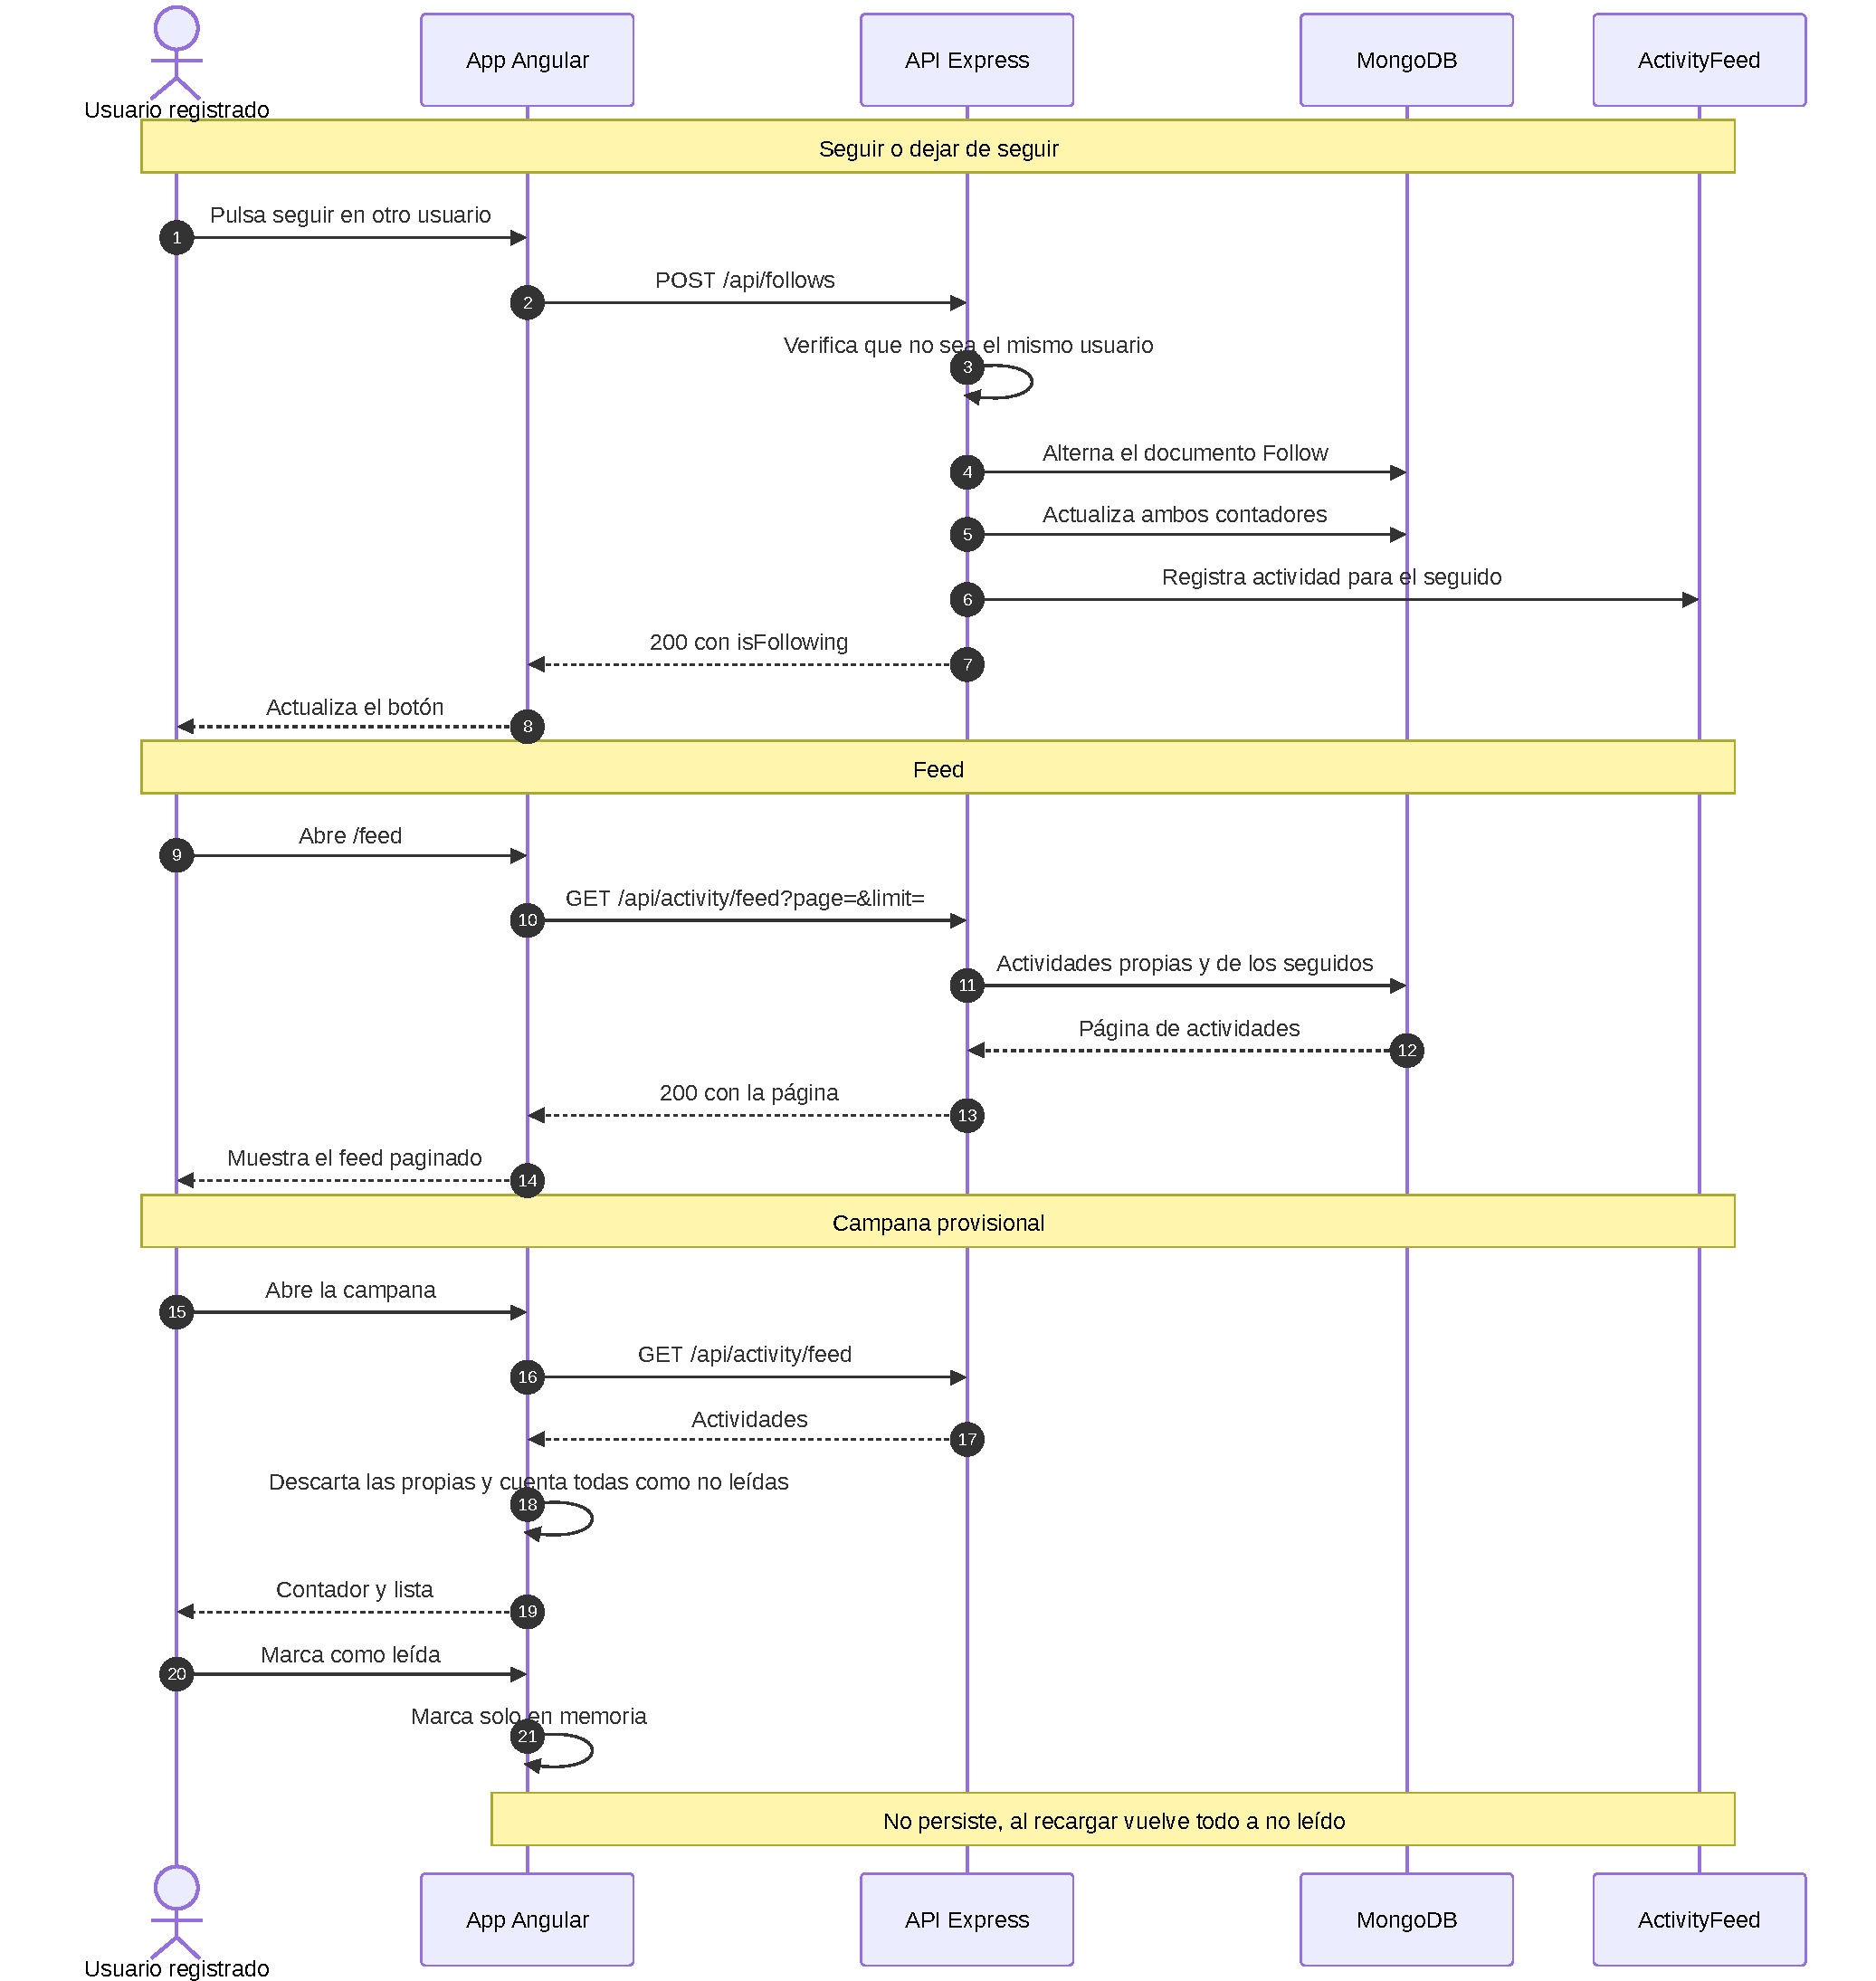
\includegraphics[width=0.72\textwidth, height=0.78\textheight, keepaspectratio]{figuras/secuencia/secuencia-seguir-usuarios-y-feed.pdf}
    \captionof{figure}{Secuencia del seguimiento entre usuarios y de la consulta del feed.}
    \label{fig:sec-feed}
\end{figure}

% =====================================================================
% 7b. DIAGRAMAS DE ESTADO
% =====================================================================
\section{Diagramas de estado}

Los diagramas de estado describen el ciclo de vida de los recursos con estados propios. Las fuentes editables se encuentran en el directorio \texttt{docs/diagramas/estado}.

\subsection{Estados de la receta}

\begin{figure}[H]
    \centering
    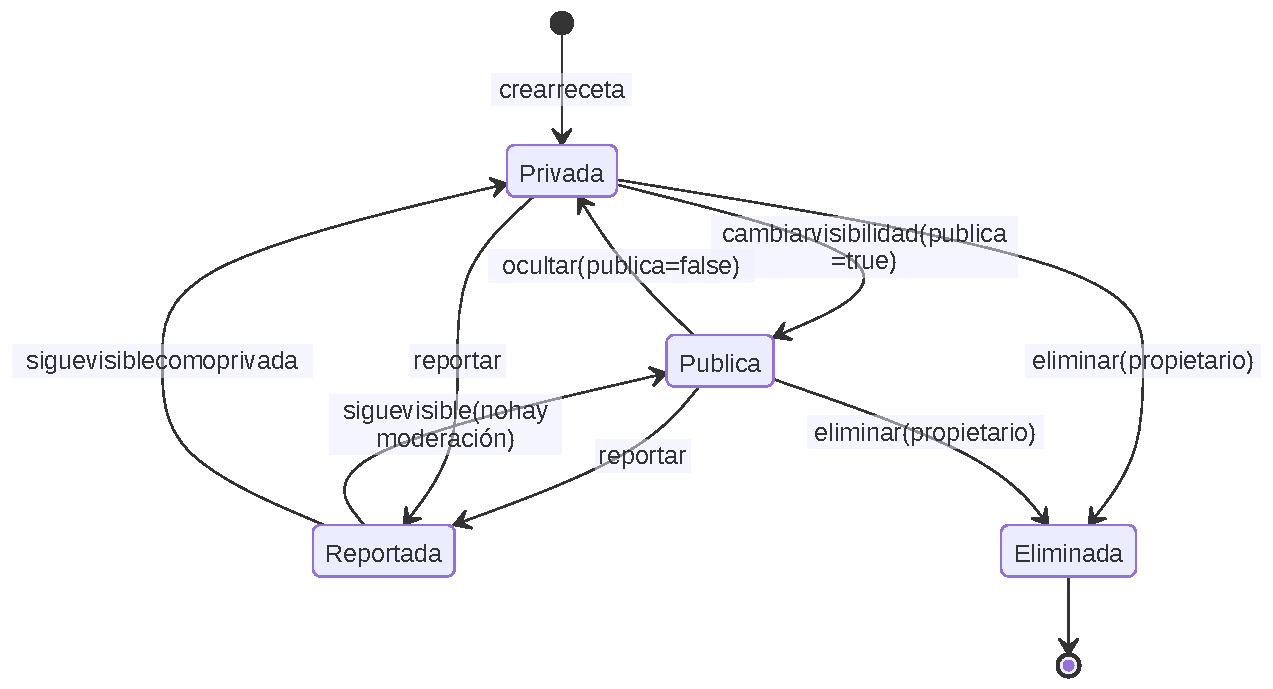
\includegraphics[width=0.72\textwidth, height=0.78\textheight, keepaspectratio]{figuras/estado/estado-receta.pdf}
    \captionof{figure}{Estados de una receta: visibilidad, reporte y eliminación.}
    \label{fig:estado-receta}
\end{figure}

La receta nace privada. La visibilidad y el reporte son atributos del documento, y el borrado es físico: no hay borrado lógico ni eliminación en cascada de comentarios, reseñas y actividades.

\subsection{Estados de la imagen}

\begin{figure}[H]
    \centering
    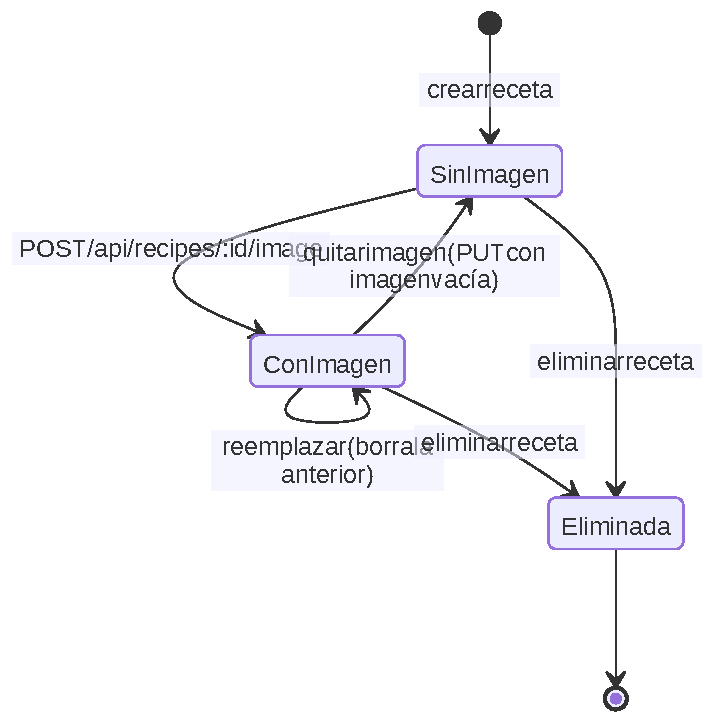
\includegraphics[width=0.72\textwidth, height=0.78\textheight, keepaspectratio]{figuras/estado/estado-imagen.pdf}
    \captionof{figure}{Estados de la imagen de una receta.}
    \label{fig:estado-imagen}
\end{figure}

Solo se conserva una imagen vigente por receta. El archivo anterior se elimina de GridFS al reemplazar, quitar o borrar la receta. La lectura es pública y usa caché inmutable.

\subsection{Estados de la campana de notificaciones}

\begin{figure}[H]
    \centering
    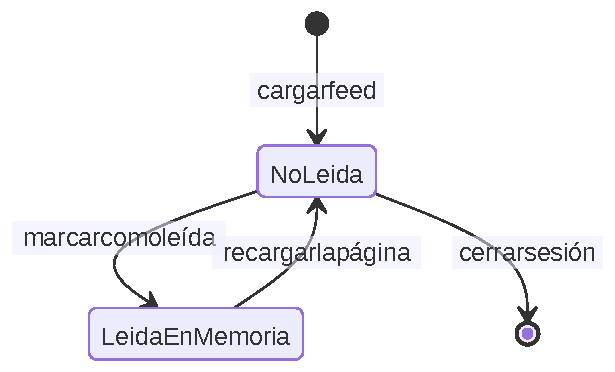
\includegraphics[width=0.72\textwidth, height=0.78\textheight, keepaspectratio]{figuras/estado/estado-campana-notificaciones.pdf}
    \captionof{figure}{Estados de la campana de notificaciones.}
    \label{fig:estado-campana}
\end{figure}

La campana es provisional: reutiliza las actividades del feed y no persiste el estado leído. Está prevista su conversión en notificaciones persistentes en un ciclo posterior.

% =====================================================================
% 7c. DIAGRAMA ER
% =====================================================================
\section{Diagrama ER}

El modelo de datos se representa mediante el diagrama entidad-relación de la base de datos MongoDB. Las colecciones principales son usuarios, recetas, comentarios, reseñas, seguimientos y actividades; las imágenes residen en GridFS.

\begin{figure}[H]
    \centering
    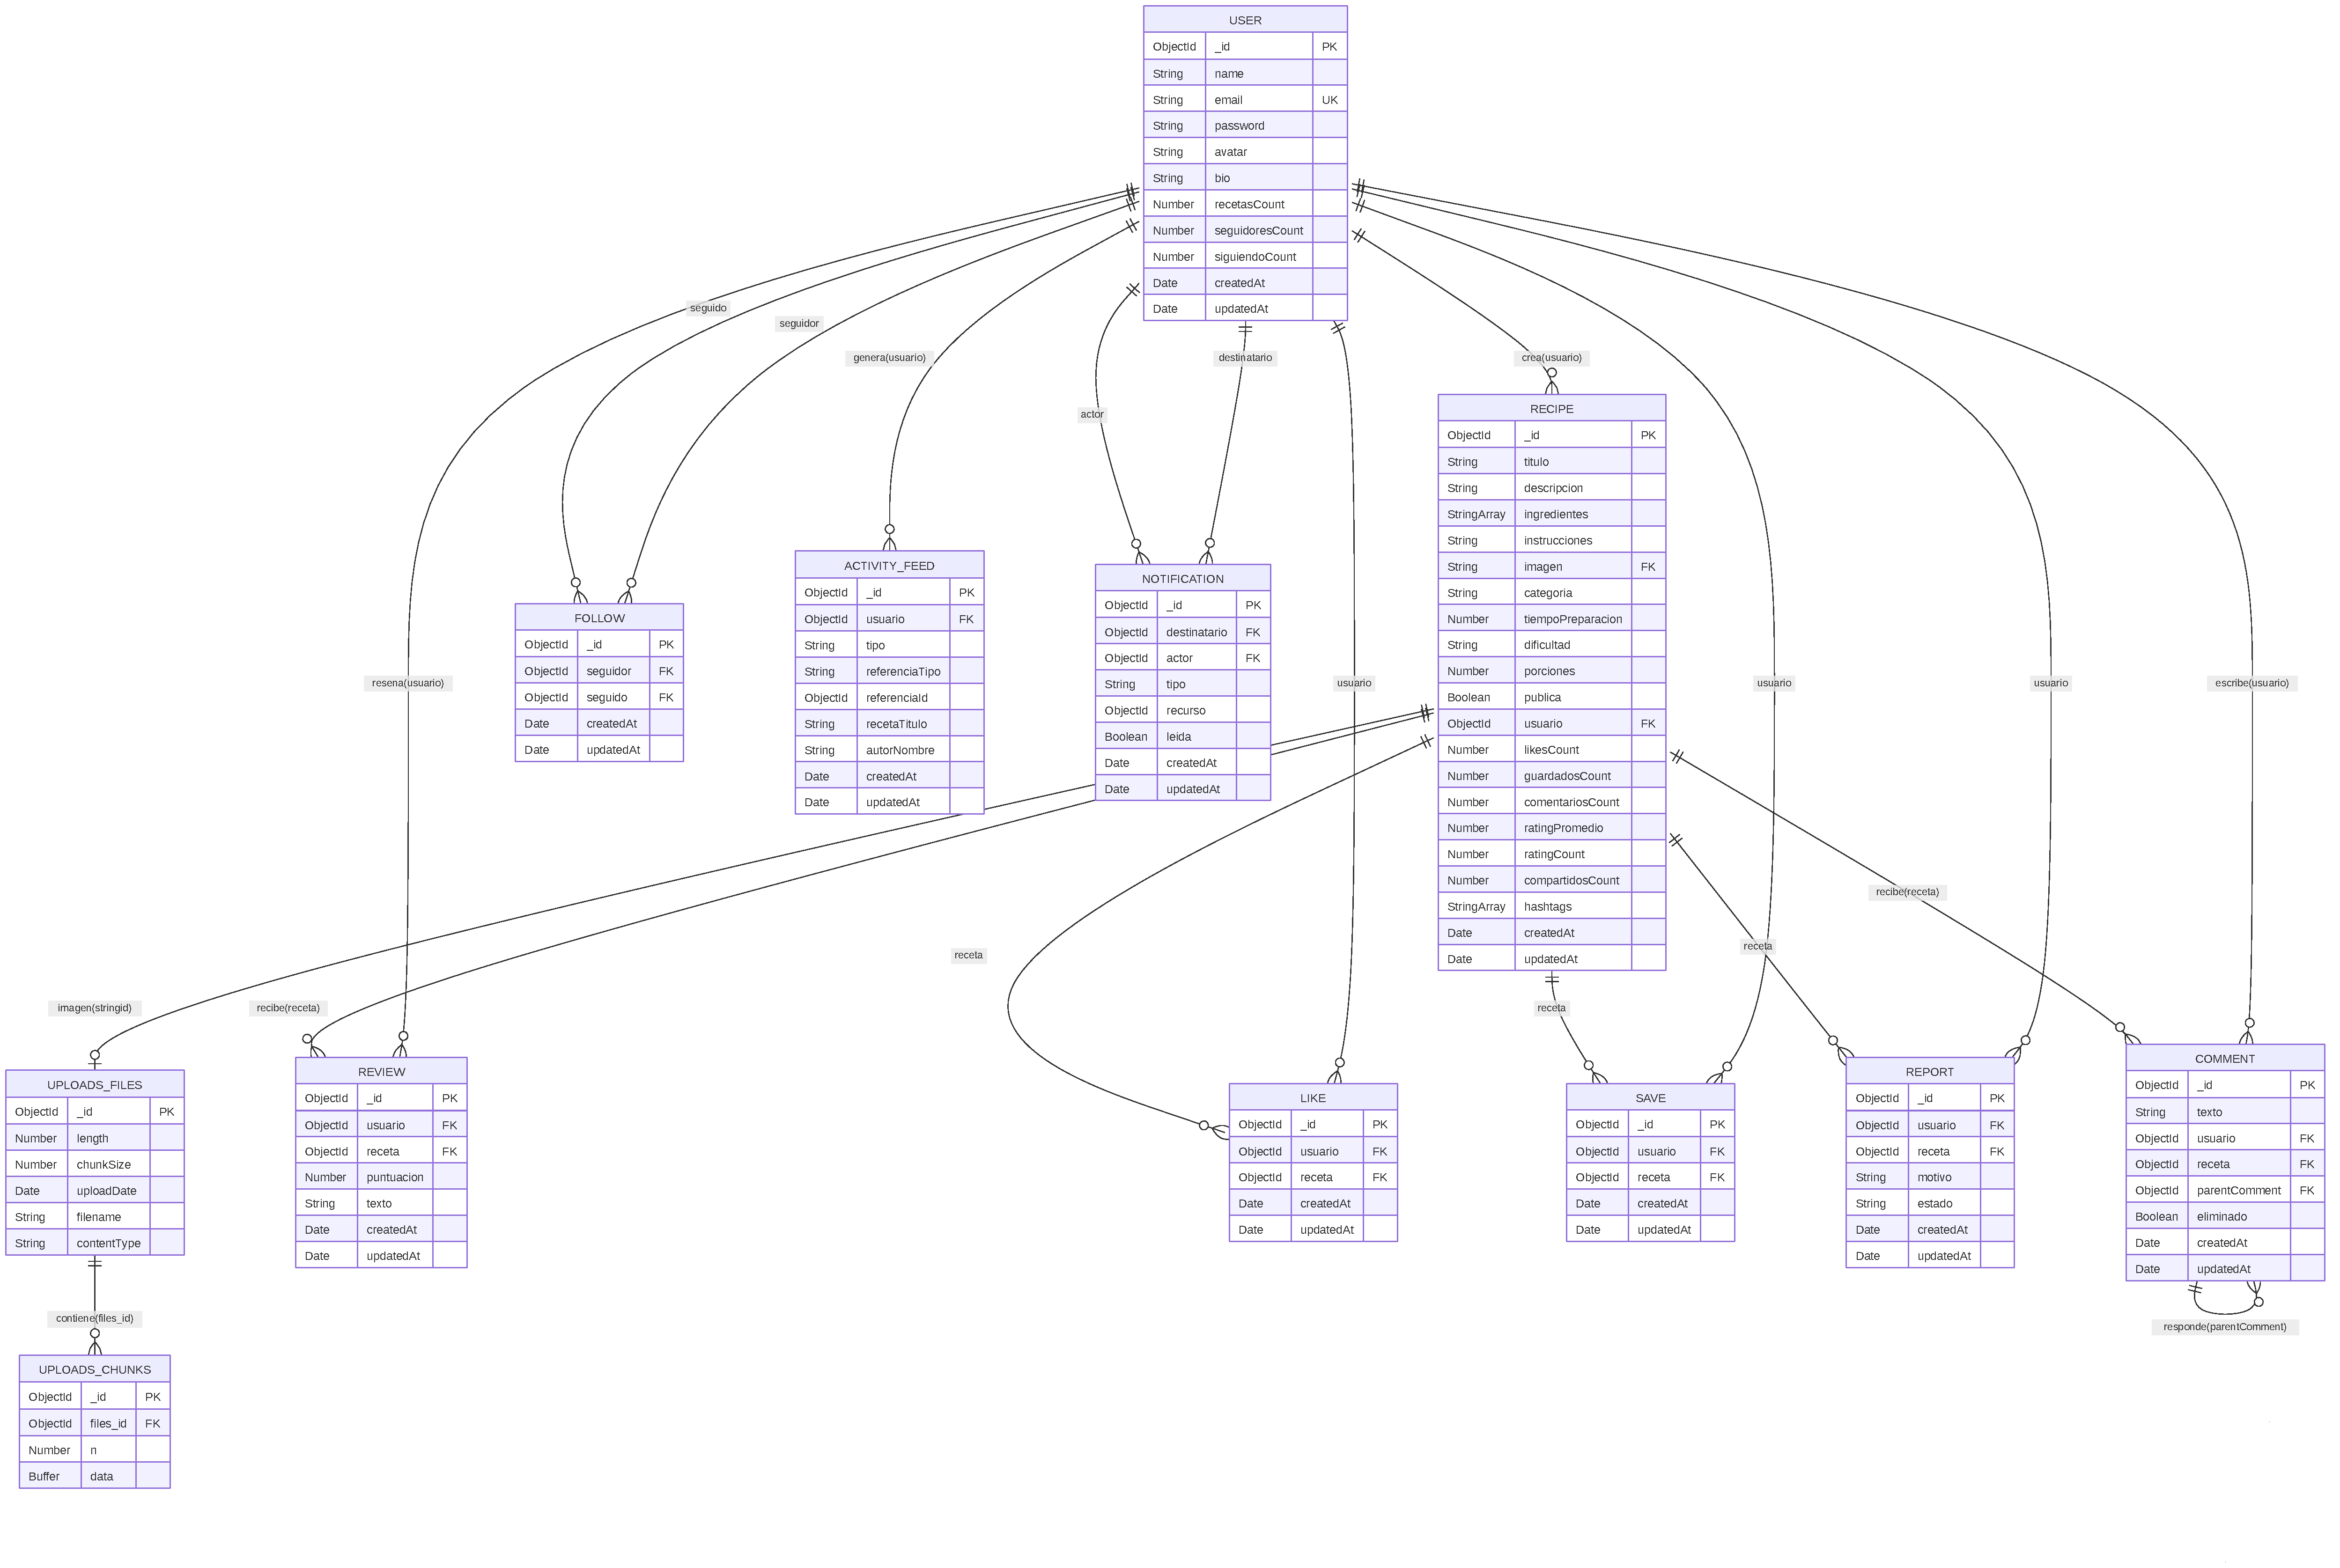
\includegraphics[width=0.72\textwidth, height=0.78\textheight, keepaspectratio]{figuras/diagrama-er.pdf}
    \captionof{figure}{Diagrama entidad-relación del sistema FoodLoop.}
    \label{fig:er}
\end{figure}

% =====================================================================
% 8. REQUERIMIENTOS NO FUNCIONALES
% =====================================================================
\section{Requerimientos no funcionales}

\subsection{Arquitectura de tres capas}

El desarrollo sigue una arquitectura de tres capas: Frontend, Backend y Base de Datos. En la capa de base de datos se utiliza MongoDB como DBMS, con GridFS para los archivos binarios. En la capa de Backend se usan servicios REST implementados en Node.js con Express y Mongoose, bajo el patrón Modelo--Vista--Controlador, consumidos desde la capa de Frontend. En la capa de Frontend se desarrollan componentes con Angular y TypeScript bajo el patrón de aplicación de página única (SPA), que se comunica con la base de datos a través de los servicios REST del Backend.

\subsection{Autenticación y autorización}

\begin{itemize}
    \item El registro y el inicio de sesión se realizan con \texttt{POST /api/auth/register} y \texttt{POST /api/auth/login}.
    \item Las contraseñas se almacenan con hash bcrypt de 10 rondas; nunca en texto claro.
    \item La sesión se representa con un JWT de 30 días que viaja en la cabecera \texttt{Authorization: Bearer}.
    \item Todas las rutas, salvo \texttt{/api/health}, las de autenticación y la lectura pública de imagen, exigen un token válido; la ausencia o invalidez del token produce \texttt{401}.
    \item La autorización es por propiedad: solo el propietario puede editar, eliminar, cambiar la visibilidad o gestionar la imagen de su receta. Una operación sobre un recurso ajeno o inexistente produce \texttt{404}.
    \item El límite de reintentos es de 10 intentos cada 15 minutos en registro e inicio de sesión.
    \item \textbf{Deuda conocida:} el cierre de sesión no invalida el token en el servidor; el \texttt{AuthGuard} del cliente comprueba la presencia del token, pero no su expiración antes de llamar al backend.
\end{itemize}

\subsection{Seguridad de datos}

\begin{itemize}
    \item El servidor conserva la propiedad de \texttt{\_id}, \texttt{usuario}, contadores, reportes y métricas: nunca se aceptan desde el cliente.
    \item Se aplica saneado de entradas (\texttt{sanitizeFields}) en comentarios, reseñas, reportes y recetas.
    \item Se aplican límites de solicitudes: \texttt{apiLimiter} global de 100 solicitudes cada 15 minutos, \texttt{authLimiter} de 10 cada 15 minutos, \texttt{socialLimiter} de 30 por minuto y \texttt{createLimiter} de 10 por minuto.
    \item Los secretos (\texttt{MONGODB\_URI}, \texttt{JWT\_SECRET}) deben residir en variables de entorno y no en el repositorio.
    \item Se distinguen de forma explícita los errores \texttt{400}, \texttt{401}, \texttt{404}, \texttt{429} y \texttt{500}.
    \item \textbf{Deuda conocida:} no se valida el \texttt{ObjectId} en todas las rutas (Mongoose lanza \texttt{CastError}); el saneado se aplica ruta a ruta en vez de globalmente; falta \texttt{app.set("trust proxy", 1)} para que el límite vea la IP real detrás de Caddy; \texttt{uploadLimiter} está definido pero no aplicado a la subida de imágenes; y hay secretos en el historial de \texttt{docker-compose.yml} pendientes de rotación.
\end{itemize}

\subsection{Almacenamiento}

\begin{itemize}
    \item Los documentos residen en MongoDB en Atlas y las imágenes en el bucket GridFS \texttt{uploads}.
    \item Solo se conserva una imagen vigente por receta; al reemplazar, quitar o borrar la receta se elimina el archivo anterior en GridFS.
    \item La optimización de imagen se realiza en el navegador con \texttt{canvas}: lado mayor de 1600 px y JPEG de calidad 0.8.
    \item El límite de carga es de 25 MB en el navegador y 5 MB en el servidor.
    \item La lectura de imagen es pública (\texttt{GET /api/recipes/image/:fileId}) y usa \texttt{Cache-Control: immutable}.
    \item \textbf{Deuda conocida:} no se verifican los bytes reales del archivo (magic bytes), solo el tipo MIME declarado; borrar una receta no elimina en cascada comentarios, reseñas ni actividad asociada.
\end{itemize}

\subsection{Integración}

\begin{itemize}
    \item El cliente Angular consume la API REST bajo el prefijo \texttt{/api}, tanto por el proxy local (\texttt{proxy.conf.json}) como por Caddy en producción.
    \item Caddy central actúa como proxy inverso y terminación TLS para \texttt{https://foodloopc.duckdns.org}.
    \item Docker Compose construye y opera los contenedores \texttt{recetario-backend} y \texttt{recetario-frontend} sobre la red externa \texttt{caddy-central\_default}.
    \item El despliegue local usa procesos Node.js y Angular independientes (\texttt{npm run dev} y \texttt{npm start}).
    \item Los envíos de archivos usan \texttt{multipart/form-data} y \texttt{multer-gridfs-storage}.
\end{itemize}

% =====================================================================
% 9. PLANIFICACIÓN DE CICLOS DE DESARROLLO
% =====================================================================
\section{Planificación de ciclos de desarrollo}

El desarrollo se organiza en ciclos incrementales. La siguiente tabla describe el alcance y las fechas de cada ciclo.

\begin{longtable}{|P{3.0cm}|L{8.7cm}|P{2.6cm}|}
\hline
\textbf{Ciclo} & \textbf{Qué abarca} & \textbf{Fechas} \\ \hline
\endfirsthead
\hline
\textbf{Ciclo} & \textbf{Qué abarca} & \textbf{Fechas} \\ \hline
\endhead
\hline
\endfoot

Uno & Configuración del entorno, autenticación y CRUD de recetas (P01, P02). & [Completar: fecha] \\ \hline

Dos & Imágenes en GridFS y visibilidad pública o privada (P03). & [Completar: fecha] \\ \hline

Tres & Red social: interacciones, comentarios, reseñas, seguimiento y feed (P04, P05, P06). & [Completar: fecha] \\ \hline

Cuatro & Notificaciones persistentes, perfil público y búsqueda global. & [Completar: fecha] \\ \hline
\end{longtable}

% =====================================================================
% 9. CRITERIOS DE ACEPTACIÓN
% =====================================================================
\section{Criterios de aceptación}

Los criterios de aceptación definen las condiciones mínimas que debe cumplir el sistema para considerarse aceptado.

\subsection{Autenticación y gestión de usuarios}

\begin{itemize}
    \item CA-01: Un visitante puede registrarse proporcionando nombre, correo y contraseña. La contraseña debe tener al menos 8 caracteres.
    \item CA-02: Al registrarse o iniciar sesión con credenciales válidas, el sistema devuelve un token JWT.
    \item CA-03: Las contraseñas no se almacenan en texto claro; se utilizan hash bcrypt de 10 rondas.
    \item CA-04: Solo las rutas públicas (/api/health, autenticación y lectura pública de imagen) pueden accederse sin token.
    \item CA-05: La API responde 401 cuando el token es ausente o inválido.
\end{itemize}

\subsection{Recetas e imágenes}

\begin{itemize}
    \item CA-06: El propietario puede crear, editar, eliminar y cambiar la visibilidad de sus recetas.
    \item CA-07: Solo el propietario puede gestionar la imagen de una receta; al reemplazarla o eliminarla, la imagen anterior se borra de GridFS.
    \item CA-08: La imagen se sirve públicamente cuando se conoce su identificador.
    \item CA-09: Las recetas nacen privadas; una receta pública es visible para otros usuarios autenticados.
\end{itemize}

\subsection{Interacciones, comentarios y reseñas}

\begin{itemize}
    \item CA-10: Un usuario autenticado puede dar/quitar me gusta, guardar y compartir recetas.
    \item CA-11: Un usuario autenticado puede comentar, responder de primer nivel y reseñar; una sola reseña por (usuario, receta).
    \item CA-12: El sistema recalcula el promedio de reseñas cuando se crea, edita o elimina una reseña.
    \item CA-13: El borrado de comentarios es lógico; las reseñas se gestionan según las reglas de la API.
\end{itemize}

\subsection{Seguimiento, feed y notificaciones}

\begin{itemize}
    \item CA-14: Un usuario no puede seguirse a sí mismo; el seguimiento es alternable y único entre par de usuarios.
    \item CA-15: El feed incluye la actividad propia y la de los usuarios seguidos, con paginación.
    \item CA-16: La campana muestra la actividad reciente de forma provisional.
\end{itemize}

\subsection{Seguridad y calidad}

\begin{itemize}
    \item CA-17: Las entradas se sanean para comentarios, reseñas, reportes y recetas.
    \item CA-18: Se aplican los límites de solicitud establecidos (api, auth, social, create).
    \item CA-19: La propiedad de los campos críticos la conserva el servidor.
    \item CA-20: El sistema distingue correctamente los códigos 400, 401, 404, 429 y 500.
\end{itemize}

% =====================================================================
% 10. FIRMAS DE ACEPTACIÓN
% =====================================================================
\section{Firmas de aceptación}

Las partes firman en señal de conformidad con el contenido de este documento de especificaciones, requerimientos y criterios de aceptación del sistema FoodLoop.

\vspace{1cm}

\begin{center}
\renewcommand{\arraystretch}{2.2}
\begin{tabular}{|P{5.0cm}|P{5.0cm}|P{4.0cm}|}
\hline
\textbf{Nombre y puesto} & \textbf{Firma y sello} & \textbf{Fecha} \\ \hline
\rule{0pt}{1.4cm}[Completar: contraparte informática] & & \\ \hline
\rule{0pt}{1.4cm}[Completar: experto del dominio] & & \\ \hline
\rule{0pt}{1.4cm}[Completar: responsable del despliegue] & & \\ \hline
\rule{0pt}{1.4cm}[Completar: autor del documento] & & \\ \hline
\end{tabular}
\end{center}

\vspace{1.5cm}
\begin{center}
\textit{Documento generado a partir de la especificación del proyecto y de la documentación técnica en \texttt{docs/}.}
\end{center}

% =====================================================================
% ANEXO A. CATÁLOGO DE LA INTERFAZ REST
% =====================================================================
\clearpage
\section*{Anexo A. Catálogo de la interfaz REST}

\small
\begin{longtable}{|P{1.8cm}|P{6.4cm}|L{6.4cm}|}
\hline
\textbf{Método} & \textbf{Ruta} & \textbf{Descripción} \\ \hline
\endfirsthead
\hline
\textbf{Método} & \textbf{Ruta} & \textbf{Descripción} \\ \hline
\endhead
\hline
\endfoot

GET & \texttt{/api/health} & Estado del servicio y de la conexión con MongoDB. \\ \hline
POST & \texttt{/api/auth/register} & Registra un usuario y devuelve el token. \\ \hline
POST & \texttt{/api/auth/login} & Inicia sesión y devuelve el token. \\ \hline
POST & \texttt{/api/recipes} & Crea una receta y asigna el propietario. \\ \hline
GET & \texttt{/api/recipes} & Lista las recetas del usuario. \\ \hline
GET & \texttt{/api/recipes?scope=public} & Lista las recetas públicas y las propias. \\ \hline
GET & \texttt{/api/recipes/:id} & Detalle de una receta propia o pública. \\ \hline
PUT & \texttt{/api/recipes/:id} & Actualiza una receta propia. \\ \hline
DELETE & \texttt{/api/recipes/:id} & Elimina una receta propia y su imagen. \\ \hline
GET & \texttt{/api/recipes/image/:fileId} & Sirve la imagen de una receta. \\ \hline
POST & \texttt{/api/recipes/:id/image} & Sube o reemplaza la imagen de una receta. \\ \hline
POST & \texttt{/api/recipes/:id/like} & Alterna el me gusta. \\ \hline
POST & \texttt{/api/recipes/:id/save} & Alterna el guardado. \\ \hline
POST & \texttt{/api/recipes/:id/share} & Incrementa el contador de compartidos. \\ \hline
POST & \texttt{/api/recipes/:id/report} & Reporta una receta con un motivo. \\ \hline
POST & \texttt{/api/comments} & Crea un comentario o respuesta. \\ \hline
GET & \texttt{/api/comments/receta/:recetaId} & Lista los comentarios de una receta. \\ \hline
PUT & \texttt{/api/comments/:id} & Edita un comentario propio. \\ \hline
DELETE & \texttt{/api/comments/:id} & Retira un comentario propio. \\ \hline
POST & \texttt{/api/reviews} & Crea una reseña. \\ \hline
GET & \texttt{/api/reviews/receta/:recetaId} & Lista las reseñas de una receta. \\ \hline
PUT & \texttt{/api/reviews/:id} & Actualiza una reseña propia. \\ \hline
DELETE & \texttt{/api/reviews/:id} & Elimina una reseña propia. \\ \hline
POST & \texttt{/api/follows} & Sigue o deja de seguir a un usuario. \\ \hline
GET & \texttt{/api/follows/followers/:userId} & Lista los seguidores de un usuario. \\ \hline
GET & \texttt{/api/follows/following/:userId} & Lista los usuarios seguidos. \\ \hline
GET & \texttt{/api/follows/check/:userId} & Indica si se sigue a un usuario. \\ \hline
GET & \texttt{/api/activity/feed} & Feed paginado de actividad. \\ \hline
GET & \texttt{/api/activity/user/:userId} & Actividad de un usuario. \\ \hline
\end{longtable}

\normalsize

% =====================================================================
% ANEXO B. ESTADOS Y SUS TRANSICIONES
% =====================================================================
\section*{Anexo B. Estados y sus transiciones}

\begin{longtable}{|P{3.4cm}|L{10.6cm}|}
\hline
\textbf{Entidad} & \textbf{Estados y transiciones permitidas} \\ \hline
\endfirsthead
\hline
\textbf{Entidad} & \textbf{Estados y transiciones permitidas} \\ \hline
\endhead
\hline
\endfoot

Receta & Nace \textit{privada}; puede alternar a \textit{pública} y de nuevo a \textit{privada}. El atributo \textit{reportada} es independiente y no cambia la visibilidad. La entidad se elimina de forma física. \\ \hline

Imagen & \textit{Sin imagen} $\rightarrow$ \textit{con imagen} (al subir); \textit{con imagen} $\rightarrow$ \textit{con imagen nueva} (al reemplazar); \textit{con imagen} $\rightarrow$ \textit{sin imagen} (al quitar o borrar la receta). Solo una imagen vigente por receta. \\ \hline

Comentario & \textit{Visible} $\rightarrow$ \textit{eliminado} de forma lógica; la respuesta de primer nivel comparte el ciclo del comentario principal. \\ \hline

Reseña & \textit{Creada} $\rightarrow$ \textit{actualizada} (por el mismo autor) $\rightarrow$ \textit{eliminada}; una sola reseña por usuario y receta. \\ \hline

Seguimiento & \textit{No sigue} $\rightarrow$ \textit{sigue} $\rightarrow$ \textit{no sigue}; pareja única entre emisor y destinatario, sin auto-seguimiento. \\ \hline

Sesión & \textit{Activa} con token válido $\rightarrow$ \textit{cerrada} localmente al eliminar el token; el token permanece válido en el servidor hasta su expiración. \\ \hline

\end{longtable}

\end{document}
